%%==================================================================%%
%% Author : Tejedo, Daniel                                          %%
%%          S�nchez Barreiro, Pablo                                 %%
%% Version: 1.0, 08/10/2012                                         %%                   %%                                                                  %%
%% Memoria del Proyecto Fin de Carrera                              %%
%% Archivo ra�z                                                     %%
%%==================================================================%%

\documentclass[a4paper,11pt]{itsas_pfc}

%=====================================================================%
%                       My imported packages                          %
%=====================================================================%
\usepackage[latin1]{inputenc}
\usepackage{longtable}
\usepackage{array}
\usepackage{url}
\usepackage{amsfonts}
\usepackage[spanish,activeacute]{babel}

% \usepackage[T1]{fontenc}
%\usepackage[scaled]{uarial}

% File with main configuration
\input{config/pfc_options.tex}

% File with some names
%
% This file has a list of internal names (variables) of LaTeX,
% of which you can change the value. For example, you can make
% chapters read "Section" instead of "Chapter".
%
\renewcommand\bibname{References}                 % thus Bibliography will read "References"
%\renewcommand{\tablename}{xxx}                   % name below each table (xxx 1: bla-bla-bla)
%\renewcommand{\figurename}{xxx}                  % name below each figure (xxx 1: bla-bla-bla)
%\renewcommand{\listtablename}{yyy}               % name for table of tables
%\renewcommand{\listfigurename}{yyy}              % name for table of figures


%=====================================================================%
%                           Authoring's details                          %
%=====================================================================%
\newcommand{\myname}{Daniel Tejedo Gonz�lez}  % name of author
\newcommand{\myboss}{Pablo S�nchez Barreiro} % name of supervisor
\newcommand{\thesistitle}{Desarrollo de un entorno para la especificaci�n y validaci�n de restricciones en �rboles de caracter�sticas con cardinalidad}

\newcommand{\englishtitle}{Development of enviroment for the specification and validation of constraints for cardinality-based feature model}
												  % work title
\newcommand{\worktype}{Proyecto Fin de Carrera}   % work type
\newcommand{\logo}{images/uc.eps}            % logo file (e.g. for the cover)

%=====================================================================%
%                     Definition of my own commands                   %
%=====================================================================%
\newcommand{\nota}[1]{\color{red}$\ll$#1$\gg$\color{black}}
\newcommand{\imp}[1]{{\small{\sf #1}}}
\newcommand{\stereotype}[1]{$\ll${\small{\sf #1}}$\gg$}
\newcommand{\todo}[1]{\color{red}$\ll$TODO: #1$\gg$\color{black}}

\setcounter{minitocdepth}{1}

\begin{document}

% Cover page
% %
% This file produces the first page of the PFC/Thesis, featuring
% the title, your name, supervisor's name and so forth.
%
% Most, if not all, content in this page is included via commands
% (e.g. \thesistitle) that have been defined in Config/pfc_options.tex
%
% Edit to your liking.
%

\thispagestyle{empty} % don't print neither page number nor headers nor footers.

%
% Use \tb to place the various items in the page. Usage:
%
% \tb{w}{h}{v}{t}
%
% where:
%
% w = paragraph width of text box (1.0 = page width)
% h = horizontal position of the center of text box (0.0 = left, 1.0 = right)
% v = vertical position of the center of text box (0.0 = top, 1.0 = bottom)
% t = text to put inside text box
%
\tb{0.8}{0.50}{0.100}{\large FACULTAD DE CIENCIAS}
\tb{0.8}{0.50}{0.130}{\Large UNIVESIDAD DE CANTABRIA}
\tb{0.8}{0.50}{0.250}{
	
\includegraphics[width=0.30\columnwidth]{images/ingInformatica.eps} \ \ \ \ \
}
\tb{0.8}{0.50}{0.390}{\LARGE \worktype}    % whether this is a PFC or a Thesis
\tb{0.8}{0.50}{0.500}{\Huge \thesistitle}  % title of the work
\tb{0.8}{0.50}{0.600}{\LARGE (\englishtitle)}  % title of the work
\tb{0.8}{0.50}{0.700}{\Large Para acceder al T�tulo de \\
					  INGENIERO EN INFORM�TICA}   % the name of the supervisor
\tb{0.2}{0.70}{0.850}{\begin{tabular}{r}
\Large Autor: \myname \\
\Large Julio 2011 \\
\end{tabular}}

\ \clearpage                       % end page here
\thispagestyle{empty} \ \clearpage % blank page


% \begin{tabular}{p{.15\textwidth}p{.50\textwidth}p{.15\textwidth}}
	\includegraphics[width=\linewidth]{\logo} & 
	\begin{center}FACULTAD DE CIENCIAS\end{center} & \\
\end{tabular}

\vspace{-15pt}

\begin{center}
INGENIER�A EN INFORM�TICA
\end{center}

\begin{center}
CALIFICACI�N DEL PROYECTO FIN DE CARRERA
\end{center}

\begin{tabular}{p{0.25\textwidth}p{0.75\textwidth}}
Realizado por:    & \myname \\ 
Director del PFC: & \myboss \\
T�tulo:           & \thesistitle  \\   
Title:            & \englishtitle \\  
\end{tabular}


Presentado a examen el d�a: 

\begin{center}
para acceder al T�tulo de \\ 
INGENIERO EN INFORM�TICA
\end{center}

\underline{Composici�n del Tribunal:} \\

\begin{tabular}{ll}
Presidente (Apellidos, Nombre): & \\
Secretario (Apellidos, Nombre): & \\
Vocal (Apellidos, Nombre): & \\
Vocal (Apellidos, Nombre): & \\
Vocal (Apellidos, Nombre): & \\
\end{tabular}

\ \\

Este Tribunal ha resuelto otorgar la calificaci�n de: ......................................

\begin{center}
\begin{tabular}{cc}
& \\
& \\
& \\
\ \ \ \ \ \ \ \ \ \ \ \
Fdo.: El Presidente 
\ \ \ \ \ \ \ \ \ \ \ \ &  
\ \ \ \ \ \ \ \ \ \ \ \
Fdo.: El Secretario  
\ \ \ \ \ \ \ \ \ \ \ \ \\
& \\
& \\
& \\
Fdo.: Vocal \ \ \ \ \ \          &         Fdo.: Vocal \ \ \ \ \ \ \\
& \\
& \\
& \\
Fdo.: Vocal \ \ \ \ \ \          &         Fdo.: El Director del PFC \ \ \ \ \ \  \\
\end{tabular}
\end{center}

\thispagestyle{empty} \



% reset page numbering
\input{config/begin.tex}

% acknowledgement
% \cdpchapter{Agradecimientos}

TODO: Aqu� se suelen poner agradecimientos si uno quiere y dedicatorias.
 % acknowledgements

% Preface
%\input{introduction/preface-lff.tex}   % preface

% Toc
% \input{config/toc.tex}

\input{Config/headers.tex}

\input{config/chapters.tex}

% Cap�tulo 1: Introducci�n
%==================================================================%
% Author : Doe Doe, John                                           %
%          S�nchez Barreiro, Pablo                                 %
% Version: 1.0, dd/mm/yyyy                                         %                   %                                                                  %
% Memoria del Proyecto Fin de Carrera                              %
% Introducci�n, archivo ra�z                                       %
%==================================================================%

%%% Schema to write a paper introduction
%% Description of Purpose
	% What problem, issue or question does this research address ?
		%
	% What limitations or failings of current understanding, knowledge, method,
	% or technologies does this research resolve ?
		%
	% What is the significance of the problem issue or question ?
		%
%% Goal statement
	% What new understanding, knowledge, methods or technologies will this
	% research generate ?
		%
	% How this address the purpose of the work ?
		%
%% Approach
	% What experiments, prototypes or studies will be done to achieve the stated % goal ?
		%
	% How will achievement or contribution of the research be demonstrated or validated ?
		%

\chapterheader{Introduction}{Introduction}
\label{chap:introduction}

% Introducci�n al cap�tulo

\chaptertoc

\section{Introducci�n}
\label{sec:intr:introduction}

TODO: Siguiendo el esquema que aparece arriba, escribir la introducci�n

\section{Motivaci�n and Contribuciones}
\label{sec:intr:motivation}

TODO: Esta secci�n es m�s para tesis doctorales que para proyectos fin de carrera. La dejamos de momento pero se podr�a eliminar

\section{Visi�n General del Proyecto}
\label{sec:intr:overview}

TODO: Esto est� bien dejarlo, pero tambi�n es suprimible

\section{Estructura del Documento}
\label{sec:intr:organization}

Esto es una especie de �ndice ampliado y se deja, suele ser bastante �til para que el que est� vago se lea esto y se acabe el problema.





 % Chapter 1

% Cap�tulo 2: Resumen del Estado del Arte
%%==================================================================%%
%% Author : Tejedo Gonz�lez, Daniel                                 %%
%%          S�nchez Barreiro, Pablo                                 %%
%% Version: 1.0, 18/11/2012                                         %%                   %%                                                                  %%
%% Memoria del Proyecto Fin de Carrera                              %%
%% Antecedentes, archivo ra�z                                       %%
%%==================================================================%%

\chapterheader{Antecedentes}{Antecedentes}
\label{chap:background}

Este cap�tulo trata de describir a grandes rasgos las t�cnicas, tecnolog�as y herramientas utilizadas para el desarrollo del presente Proyecto Fin de Carrera. En primer lugar, se introducir� el caso de estudio que se utilizar� de forma recurrente a lo largo del proyecto, que es una l�nea de productos software para software de control para hogares inteligentes. Para ello se describen en primer lugar diversos conceptos relacionados el dominio del proyecto, como son las l�neas de productos software y los �rboles de caracter�sticas. A continuaci�n, se describen dos principales herramientas de Ingenier�a de Lenguajes Dirigida por Modelos utilizadas: \emph{Ecore} y \emph{EMFText}. Por �ltimo, se describe brevemente la arquitectura de plugins de Eclipse, dado que nuestro proyecto deb�a integrarse en dicho entorno.

\chaptertoc

\section{Caso de Estudio: Software para Hogares Inteligentes}
\label{sec:back:spl}
%%==================================================================%%
%% Author : Perez Ruiz, Alejandro                                   %%
%% Author : Pablo S�nchez                                           %%
%% Version: 1.1, 13/06/2011                                         %%
%%                                                                  %%
%% Memoria del Proyecto Fin de Carrera                              %%
%% Planificacion/CasoEstudio                                        %%
%%==================================================================%%

El objetivo �ltimo del presente proyecto es la construcci�n de una l�nea de productos software sobre la plataforma .NET para hogares automatizados y/o inteligentes.

%%===========================================================================%%
%% NOTA(Pablo): Dado el contexto del proyecto, este p�rrafo no interesa      %%
%%===========================================================================%%
%%
%% Se ha elegido este dominio de aplicaci�n por ser un dominio donde el uso
%% de un enfoque basado en L�neas de Productos Software se hace casi
%% imperativo, debido a la gran variabilidad existente en estos productos.
%% Esta  variabilidad se debe tanto a motivos de hardware, dado que los
%% dispositivos a ser controlados e interconectados pueden variar enormemente,
%% como funcionales, dado que existen multitud de funcionalidades que se pueden
%% ofrecer de manera opcional o alternativa al usuario, no siendo necesario que
%% un determinado hogar las posea todas ellas.
%%
%%===========================================================================%%

El objetivo de estos hogares es aumentar la comodidad y seguridad de sus habitantes, as� como hacer un uso m�s eficiente de la energ�a consumida. Los ejemplos m�s comunes de tareas automatizadas dentro de un hogar inteligente son el control de las luces, ventanas, puertas, persianas, aparatos de fr�o/calor, as� como otros dispositivos, que forman parte de un hogar. Un hogar inteligente tambi�n busca incrementar la seguridad de sus habitantes mediante sistemas automatizados de vigilancia y alerta de potenciales situaciones de riesgo. Por ejemplo, el sistema deber�a encargarse de detecci�n de humos o de la existencia de ventanas abiertas cuando se abandona el hogar.

El funcionamiento de un hogar inteligente se basa en el siguiente esquema: (1) el sistema lee datos o recibe datos de una serie de sensores; (2) se procesan dichos datos; y (3) se activan los actuadores para realizar las acciones que correspondan en funci�n de los datos recibidos de los sensores.

Todos los sensores y actuadores se comunican a trav�s de un dispositivo especial denominado puerta de enlace (\emph{Gateway}, en ingl�s). Dicho dispositivo se encarga de coordinar de forma adecuada los diferentes dispositivos existentes en el hogar, de acuerdo a los par�metros y preferencias especificados por los habitantes del mismo. Los habitantes del hogar se comunicar�n con la puerta de enlace a trav�s de una interfaz gr�fica.
Este proyecto tiene como objetivo el desarrollo de un hogar inteligente como una l�nea de productos software, con un n�mero variable de plantas y habitaciones. El n�mero de habitaciones por planta es tambi�n variable. La l�nea de productos deber� ofrecer varios servicios, que podr�n ser opcionalmente incluidos en la instalaci�n del software para un un hogar determinado. Dichos servicios se clasifican en funciones b�sicas y complejas, las cuales describimos a continuaci�n.

\paragraph{Funciones b�sicas} \ \\

\begin{enumerate}
\item \emph{Control autom�tico de luces:} Los habitantes del hogar deben ser capaces de encender, apagar y ajustar la intensidad de las diferentes luces de la casa. El n�mero de luces por habitaci�n es variable. El ajuste debe realizarse especificando un valor de intensidad.
\item \emph{Control autom�tico de ventanas:} Los residentes tienen que ser capaces de controlar las ventanas autom�ticamente. De tal modo que puedan indicar la apertura de una ventana desde las interfaces de usuario disponibles.
\item \emph{Control autom�tico de persianas:} Los habitantes podr�n subir y bajar las persianas de las ventanas de manera autom�tica.
\item \emph{Control autom�tico de temperatura:} El usuario ser� capaz de ajustar la temperatura de la casa. La temperatura se medir� siempre en grados celsius.
\end{enumerate}

\paragraph{Funciones complejas} \ \\

\begin{enumerate}
\item \emph{Control inteligente de energ�a:} Esta funcionalidad trata de coordinar el uso de ventanas y aparatos de fr�o/calor para regular la temperatura interna de la casa de manera que se haga un uso m�s eficiente de la energ�a. Por ejemplo, si se recibe la orden de calentar la casa, a la vez que se activan los radiadores se cerrar�n las ventanas para evitar las p�rdidas de calor.
\item \emph{Presencia simulada:} Para evitar posibles robos, cuando los habitantes abandonen la casa por un periodo largo de tiempo, se deber� poder simular la presencia de personas en las casas. Hay dos opciones de simulaci�n (no exclusivas):
	\begin{enumerate}
	\item \emph{Simulaci�n de las luces:} Las luces se deber�n apagar y encender para simular la presencia de habitantes en la casa.
	\item \emph{Simulaci�n de persianas:} Las persianas se deber�n subir y bajar autom�tica para simular la presencia de individuos dentro de la casa.
	\end{enumerate}
\end{enumerate}

Todas estas funciones son opcionales. Las personas interesadas en adquirir el sistema podr�n incluir en una instalaci�n concreta de este software el n�mero de funciones que ellos deseen. La siguiente secci�n describe la planificaci�n general realizada para desarrollar este caso de estudio.


\section{L�neas de producto software}
\label{sec:back:spl}
%=============================================================================%
% Author : Alejandro P�rez Ruiz                                               %
% Author : Pablo S�nchez Barreiro                                             %
% Version: 1.1, 10/06/2011                                                    %
% Master Thesis: Background/Software Product Lines                            %
%=============================================================================%

El objetivo de una \emph{l�nea de productos software}~\cite{pohl:2005,kakola:2006} es crear una infraestructura adecuada a partir de la cual se puedan derivar, tan autom�ticamente como sea posible, productos concretos pertenecientes a una familia de productos software. Una familia de productos software es un conjunto de aplicaciones software similares, que por tanto comparten una serie de caracter�sticas comunes, pero que tambi�n presentan variaciones entre ellos.

Un ejemplo cl�sico de familia de productos software es el software que se encuentra instalado por defecto en un tel�fono m�vil. Dicho software contiene una serie de facilidades comunes, tales como agenda, recepci�n de llamadas, env�o de mensajes de texto, etc. No obstante, dependiendo de las capacidades y la gama del producto, �ste puede presentar diversas funcionalidades opcionales, tales como env�o de correos electr�nicos, posibilidad de conectarse a Internet mediante red inal�mbrica, radio, etc.

La idea de una l�nea de productos software es proporcionar una forma automatizada y sistem�tica de construir productos concretos dentro de una familia de productos software mediante la simple especificaci�n de qu� caracter�sticas deseamos incluir dentro de dicho producto. Esto representa una alternativa al enfoque tradicional de desarrollo software, el cual se basaba simplemente en seleccionar el producto m�s parecido dentro de la familia al que queremos construir y adaptarlo manualmente.

El proceso de creaci�n de l�neas de producto software conlleva dos fases: \emph{ingenier�a del dominio} (en ingl�s,  \emph{Domain Engineering}) e \emph{ingenier�a de aplicaci�n} (en ingl�s, \emph{Application Engineering}) (laFfigura~\ref{back:fig:domainAplicEng} ilustra el proceso para ambas fases). La \emph{ingenier�a del dominio} tiene como objetivo la creaci�n de la infraestructura o arquitectura de la l�nea de productos, la cual permitir� la r�pida, o incluso autom�tica, construcci�n de sistemas software espec�ficos pertenecientes a la familia de productos. La \emph{ingenier�a de aplicaci�n} utiliza la infraestructura creada anteriormente para crear aplicaciones espec�ficas adaptadas a las necesidades de cada usuario en concreto.

\begin{figure}[!tb]
  \centering
	\includegraphics[width=.95\linewidth]{background/domainAplicationEngineering.eps} \\
  \caption{Proceso de desarrollo de una l�nea de productos software}
  \label{back:fig:domainAplicEng}
\end{figure}

En la fase de ingenier�a del dominio, el primer paso a realizar ser�a un an�lisis de qu� caracter�sticas de la familia de productos son variables y por qu� y c�mo son variables. Esta parte es la que se conoce como \emph{an�lisis o especificaci�n de la variabilidad} (Figura~\ref{back:fig:domainAplicEng}, punto 1). A continuaci�n, se ha de dise�ar una arquitectura o marco de trabajo para la familia de productos software que permita soportar dichas variaciones. Esta actividad se conoce como \emph{realizaci�n o dise�o de la variabilidad} (Figura~\ref{back:fig:domainAplicEng}, punto 2). El siguiente paso es establecer una serie de reglas que especifiquen como hay que instanciar la arquitectura previamente creada de acuerdo con las caracter�sticas seleccionadas por cada cliente. Esta fase es la que se conoce como \emph{correspondencia entre especificaci�n y dise�o de la variabilidad} (Figura~\ref{back:fig:domainAplicEng}, punto 3).

En la fase de ingenier�a de aplicaci�n, se crear�a una \emph{configuraci�n}, que no es m�s que una selecci�n de caracter�sticas que un usuario desea incluir en su producto (Figura~\ref{back:fig:domainAplicEng}, punto 4). En el caso ideal, usando esta configuraci�n, deber�amos poder ejecutar las reglas de correspondencia entre especificaci�n y dise�o de la variabilidad para que la arquitectura creada en la fase de ingenier�a del dominio se adaptase autom�ticamente generando un producto concreto espec�fico acorde a las necesidades concretas del usuario (Figura~\ref{back:fig:domainAplicEng}, punto 5). En caso no ideal, dichas reglas de correspondencia deber�n ejecutarse a mano, lo cual suele ser un proceso tedioso, largo, repetitivo y propenso a errores.

Este proyecto se centra en la primera etapa de este proceso de desarrollo, es decir en el an�lisis de la variabilidad de una familia de productos software mediante �rboles de caracter�sticas. La siguiente secci�n proporciona una breve pero completa descripci�n acerca del funcionamiento de los �rboles de caracter�sticas.


\section{�rboles de caracter�sticas}
\label{sec:back:fmodels}
%%==================================================================%%
%% Author : Tejedo Gonz�lez, Daniel                                 %%
%%          S�nchez Barreiro, Pablo                                 %%
%% Version: 1.0, 18/11/2012                                         %%                   %%                                                                  %%
%% Memoria del Proyecto Fin de Carrera                              %%
%% Antecedentes, �rboles de caracter�sticas                                    %%
%%==================================================================%%

El objetivo de las l�neas de productos software es crear la infraestructura para la r�pida  producci�n de sistemas software para un segmento de mercado espec�fico, donde estos sistemas software son similares, y aunque comparten un subconjunto de caracter�sticas comunes, tambi�n presentan variaciones entre ellos ~\ref{} ~\ref{} ~\ref{} ~\ref{}.

El principal logro en las l�neas de productos software es, construir productos espec�ficos lo m�s autom�ticamente posible a partir de un conjunto de elecciones y decisiones adoptadas sobre un modelo com�n, conocido como modelo de referencia, que representa la familia completa de productos que la l�nea de productos software cubre.

El desarrollo de l�neas de producto software se compone de dos procesos de desarrollo software diferentes pero �ntimamente relacionados, conocidos como ingenier�a del dominio e ingenier�a de la aplicaci�n.

En el nivel de ingenier�a del dominio, comenzamos por los documentos de requisitos que describen una familia de productos similares para un segmento de mercado espec�fico. Entonces, dise�amos una arquitectura e implementaci�n de referencia para esta familia de productos. Esta arquitectura de referencia contiene los elementos que son comunes para todos los productos de la familia.

En el nivel de ingenier�a de la aplicaci�n, comenzamos un documento de requisitos de un producto espec�fico. Este documento estable las variaciones espec�ficas que deben ser incluidas en este producto concreto. Con esta informaci�n, introducimos los cambios en la arquitectura y en la implementaci�n de referencia, y se deber�a obtener como resultado un producto software �nico.

Para ser capaces de completar con �xito la tarea correspondiente a ingenier�a del dominio, una de las cuestiones clave es establecer una forma de especificar los productos software que una l�nea de productos es capaz de productor, y aqu� es donde entran en juego los �rboles de caracter�sticas o Modelos de Caracter�sticas. Los productos de una l�nea de productos software se diferencian por sus caracter�sticas, siendo una caracter�stica un incremento en la funcionalidad del producto, o m�s formalmente, "una caracter�stica es una propiedad de un sistema que es relevante a algunos stakeholders y es usada para capturar propiedades comunes o diferenciar entre sistemas de una misma familia" ~\ref{}. De este modo un producto queda representado por las caracter�sticas que posee. 

Para poder capturar las divergencias y caracter�sticas comunes entre los distintos productos, los modelos de caracter�sticas organizan el conjunto de caracter�sticas jer�rquicamente mediante las siguientes relaciones entre ellos: (1) relaci�n entre una o varias caracter�sticas padre y un conjunto de caracter�sticas hijas o subcaracter�sticas y (2) relaciones no jer�rquicas del tipo "si la caracter�stica A aparece, entonces la B se debe excluir".

Por otro lado, un modelo de caracter�sticas debe poder representar la cardinalidad de las caracter�sticas, por motivos tanto de comprensi�n (es mucho mejor contar con un �rbol de 8 nodos que con uno de 100, teniendo ambos un significado equivalente), como de funcionalidad, ya que permite expresar ciertas restricciones que de no contar con la cardinalidad no podr�an expresarse. 

Las posibles relaciones que pueden darse en un �rbol de caracter�sticas (mostradas gr�ficamente en la figura \ref{fig6}) son las siguientes:

\begin{figure}[t]
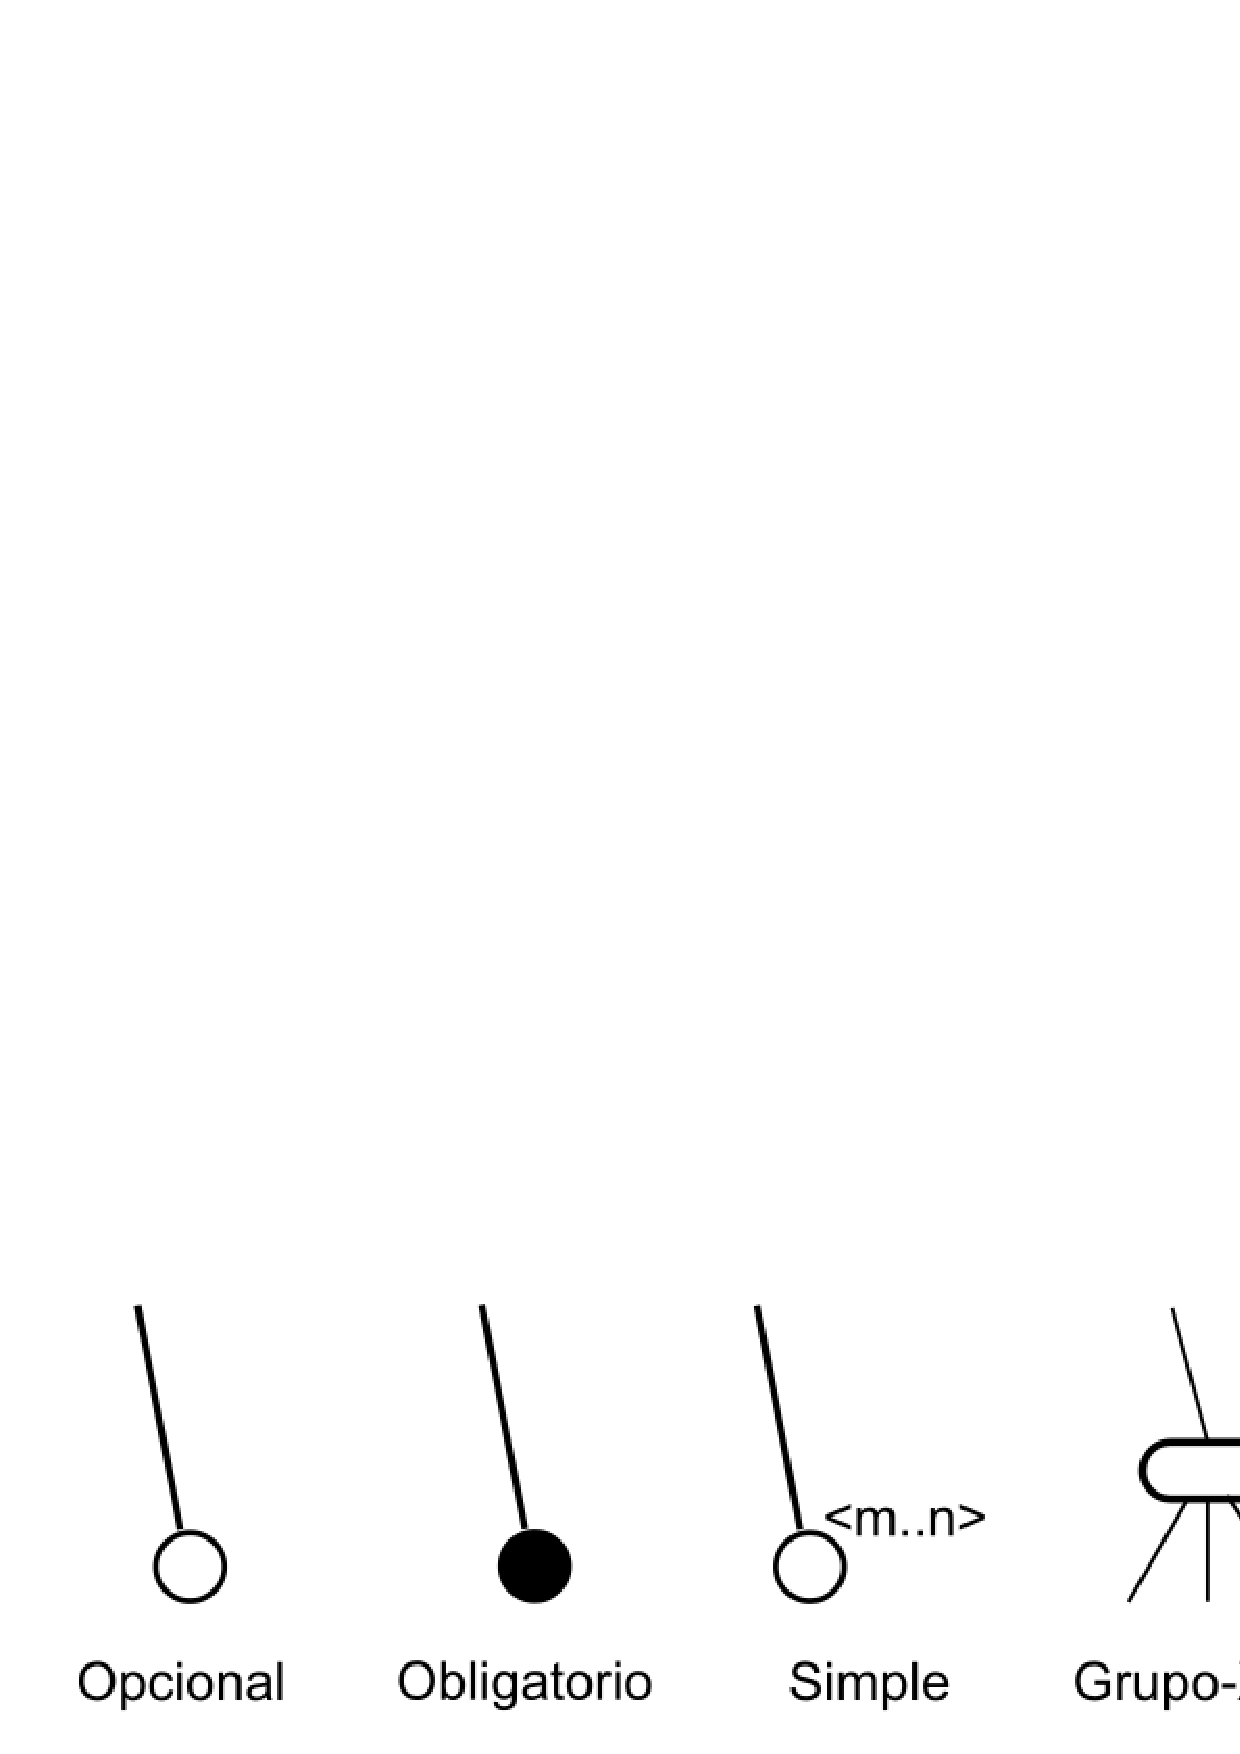
\includegraphics[scale=0.35]{background/relations.jpg}
\caption{Distintos tipos de relaciones en un modelo de caracter�sticas }
\label{fig6}
\end{figure}

1 - Opcional: La caracter�stica hija puede estar o no estar seleccionada
2 - Obligatoria: La caracter�stica es requerida.
3 - Simple: La caracter�stica tendr� una cardinalidad <m,n>, siendo m y n n�meros enteros que denotan el m�nimo y el m�ximo respectivamente de caracter�sticas que podemos seleccionar.
4 - Grupo-xor: S�lo una de las caracter�sticas pertenecientes al grupo ser� seleccionada.
5 - Grupo-or: Podremos seleccionar como m�nimo una de las subcaracter�sticas, y como m�ximo todas.
6 - Grupo simple: El n�mero de caracter�sticas seleccionadas del grupo vendr� dado por su cardinalidad <m,n>.

Adem�s se podr�n disponer de restricciones de usuario m�s complejas, que son las que se han implementado en el editor de especificaci�n y validaci�n de restricciones desarrollado en este proyecto.

\begin{figure}[t]
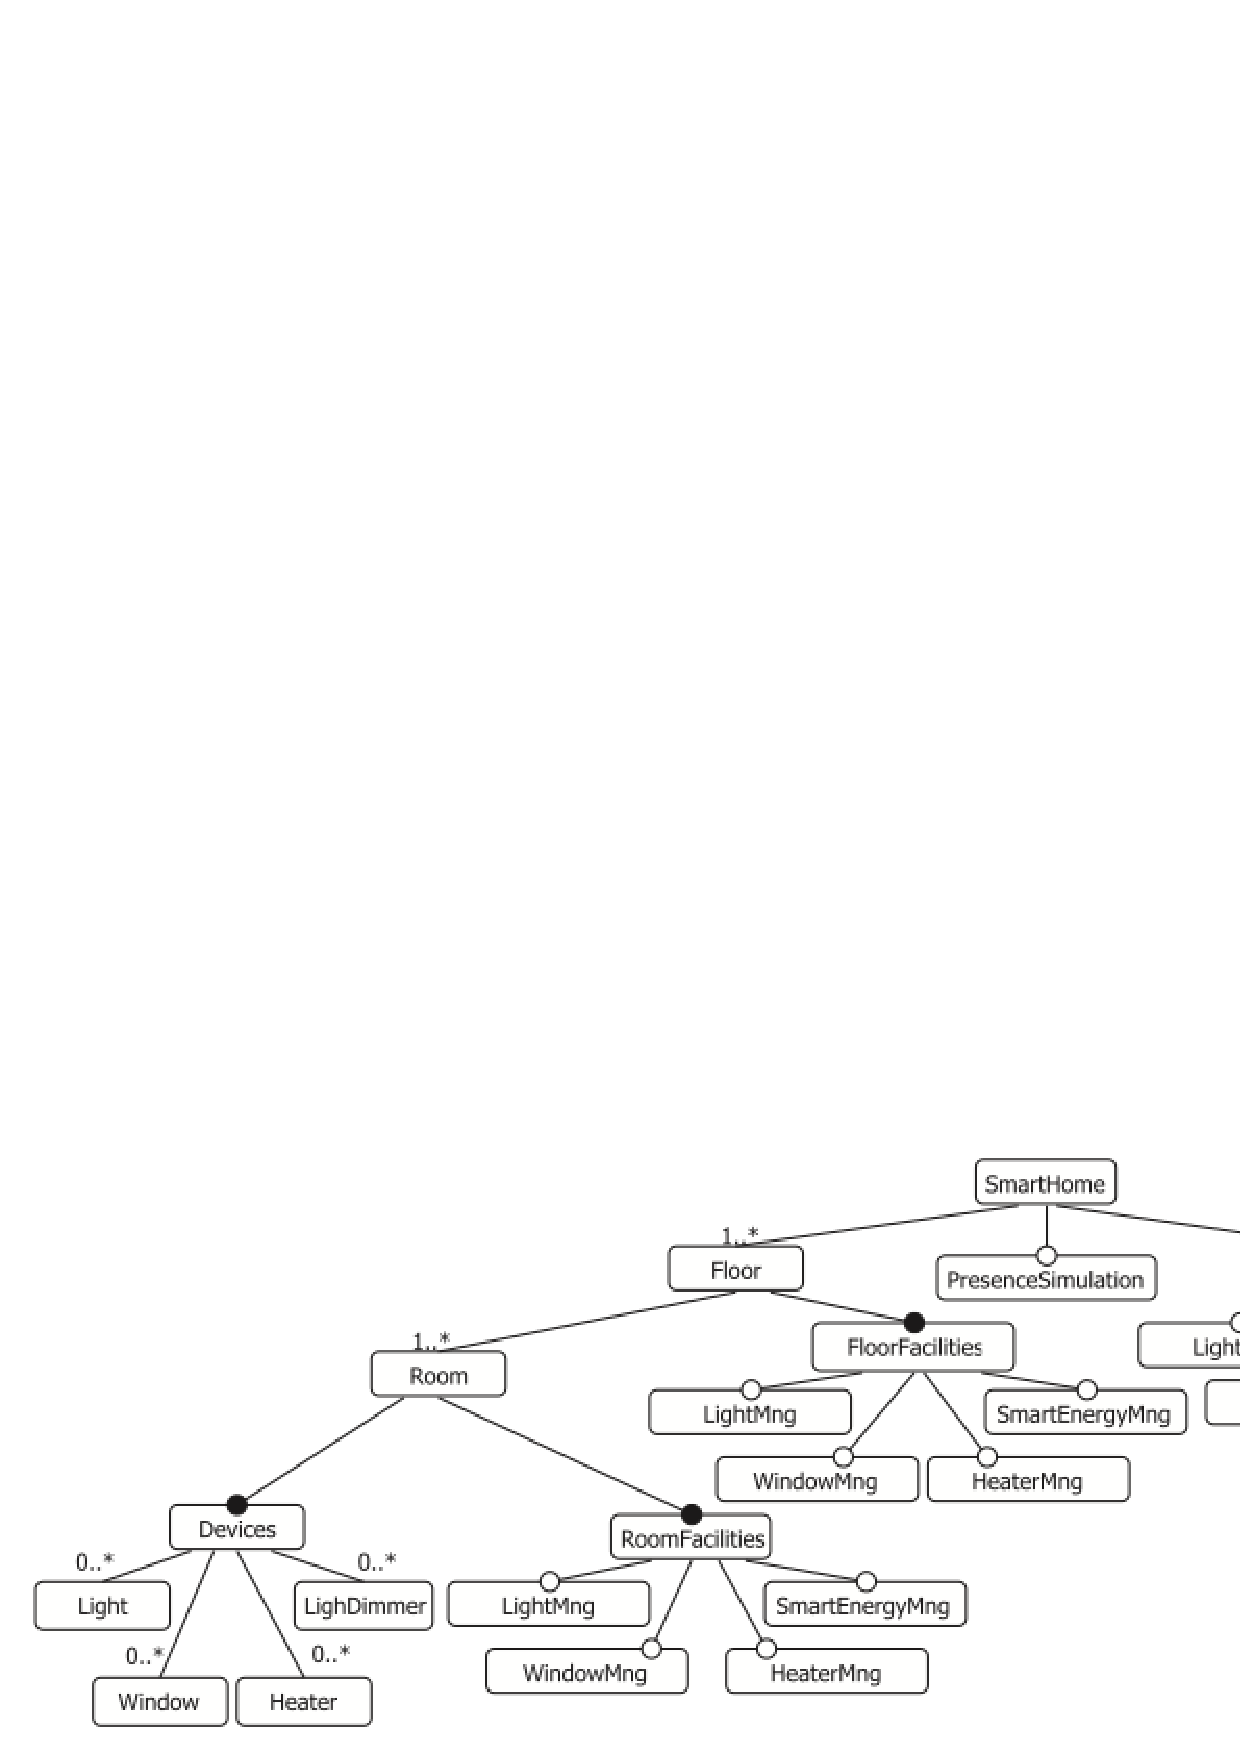
\includegraphics[scale=0.5]{background/featuremodel.jpg}
\caption{�rbol de caracter�sticas para crear una SmartHome }
\label{fig7}
\end{figure}

La figura \ref{fig7} muestra un ejemplo de modelo de caracter�sticas. En este caso se trata de un modelo de una casa inteligente o SmartHome, a trav�s del cual, seleccionando ciertas caracter�sticas u otras podremos construir qu� tipo de casa queremos. Cada una de las m�ltiples casas diferentes que podamos construir es lo que se denonima una especializaci�n o configuraci�n de nuestro modelo de caracter�sticas.

El proceso de crear una configuraci�n a partir de un modelo de caracter�sticas se conoce como proceso de configuraci�n o proceso de especializaci�n. Consiste en transformar un modelo de caracter�sticas de tal forma que el modelo resultante sea un subconjunto de las posibles configuraciones denotadas por el primer modelo. La figura \ref{fig8} muestra una posible configuraci�n para el modelo de caracter�sticas de la figura \ref{fig7}.

\begin{figure}[t]
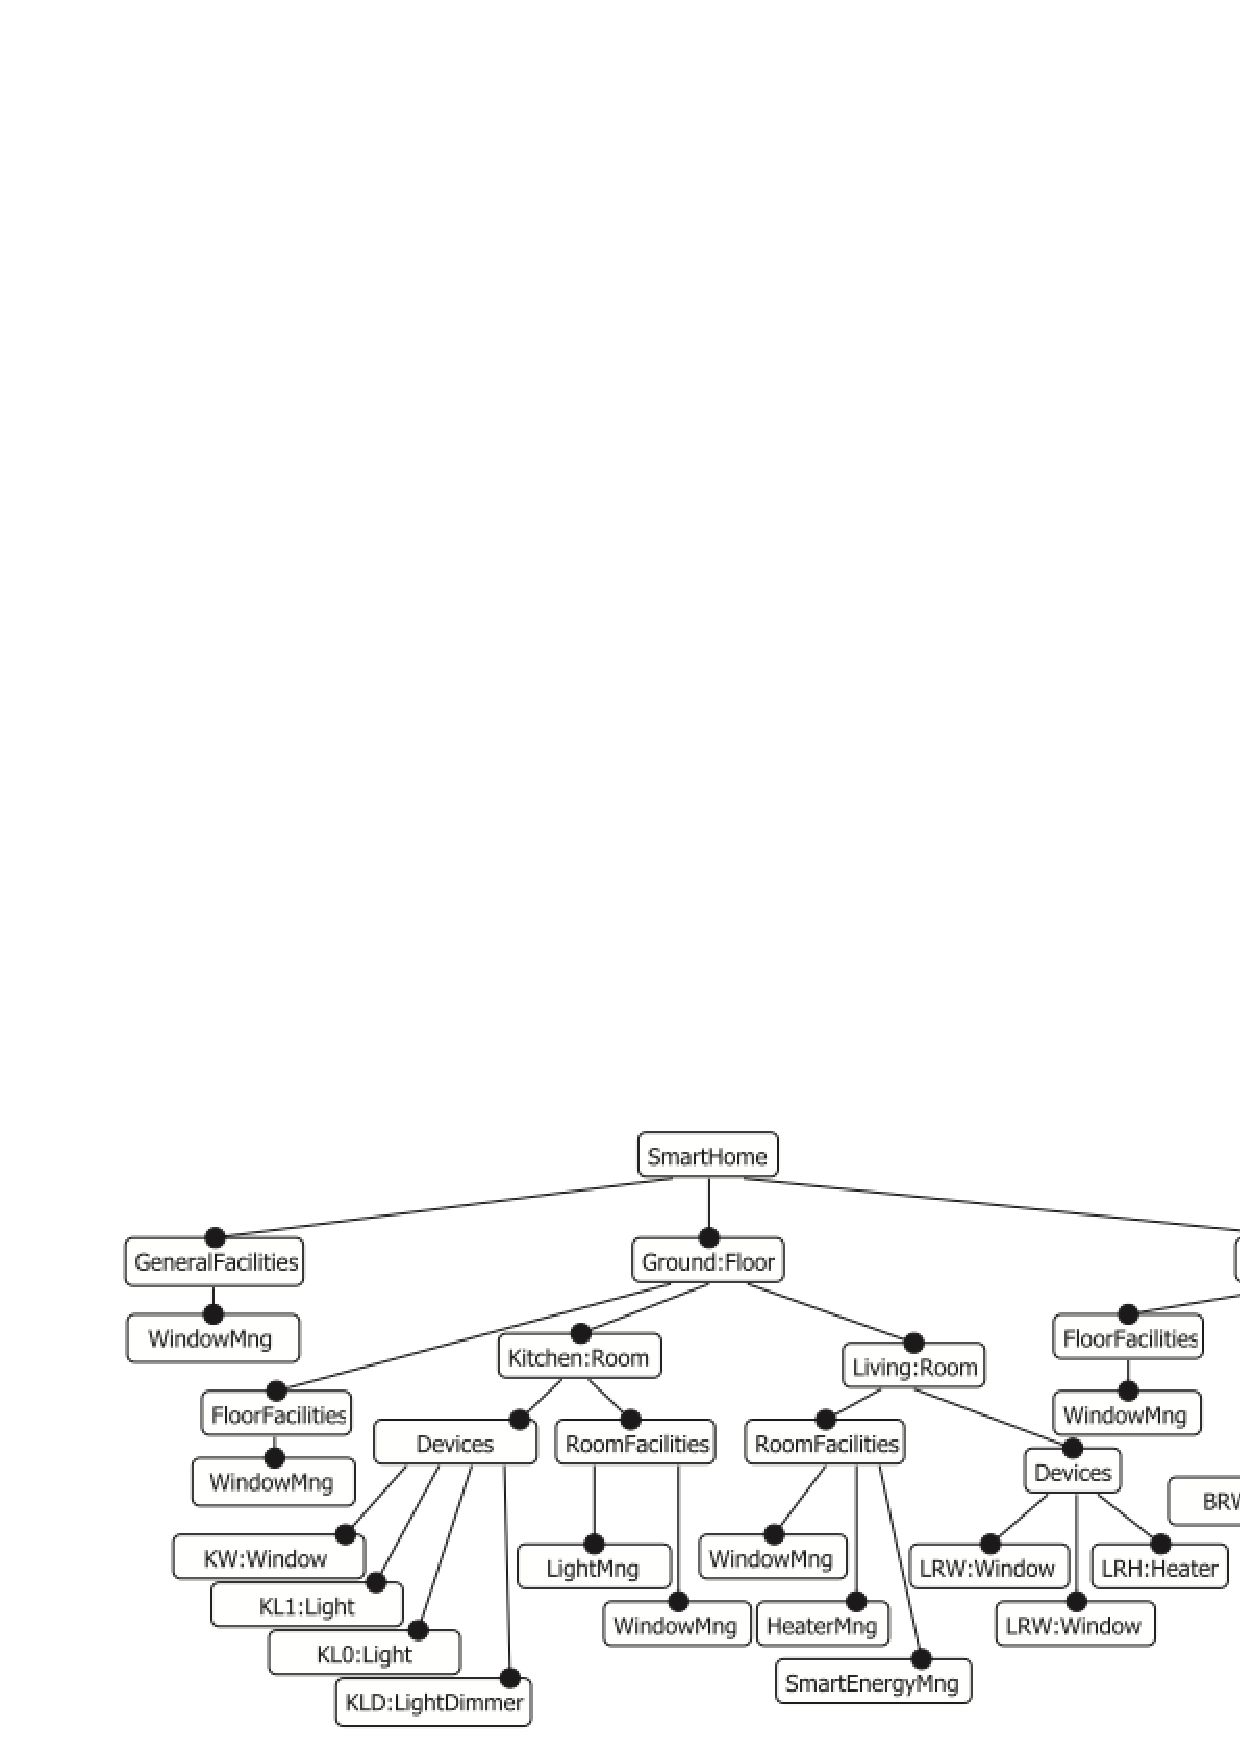
\includegraphics[scale=0.5]{background/configuration.jpg}
\caption{Especializaci�n del modelo de la figura \ref{fig7}, que representa una de las posibles casas que se pueden construir }
\label{fig8}
\end{figure}

La relaci�n entre un diagrama de caracter�sticas y una configuraci�n es an�loga a la existente entre una clase y una de sus instancias en programaci�n orientada a objetos.







\section{\emph{Eclipse Modelling Framework}}
\label{sec:back:ecore}
%%==================================================================%%
%% Author : Tejedo Gonz�lez, Daniel                                 %%
%%          S�nchez Barreiro, Pablo                                 %%
%% Version: 1.0, 18/11/2012                                         %%                  
%%                                                                  %%
%% Memoria del Proyecto Fin de Carrera                              %%
%% Antecedentes, ecore                                              %%
%%==================================================================%%

EMF \emph{Eclipse Modeling Framework}~\cite{steinberg:2008} es un \emph{plug-in} para Eclipse~\cite{clayberg:2008} que permite elaborar metamodelos. Pera ello proporciona un lenguaje de metamodelado denominado Ecore, el cual se ha convertido en el est�ndar \emph{de facto} para la realizaci�n de metamodelos. Utilizando Ecore se pueden crear metamodelos de forma gr�fica usando una notaci�n muy similar a la los diagramas de clases de UML. La Figura~\ref{fig:sle:metamodeloGrafo} muestra un sencillo ejemplo de metamodelo en Ecore (ver Secci�n~\ref{sec:intr:sle} para m�s detalles). EMF tambi�n incorpora una herramienta para la validaci�n reglas adicionales que no puedan ser especificadas a nivel de del metamodelo. 
 
EMF permite que, a partir de un metamodelo especificado en Ecore, podamos, utilizando diversos generadores de c�digo, crear autom�ticamente un conjunto de clases que nos permiten manipular dichos modelos a nivel de c�digo. Dichas clases se pueden adem�s distribuir como \emph{plug-in} para el entorno Eclipse.

Adem�s, al haberse convertido en est�ndar \emph{de facto} para el desarrollo de metamodelos, Ecore es compatible con multitud de herramientas para Ingenier�a de Lenguajes Dirigida por Modelos, como EMFText, la cual se describe en la siguiente secci�n, o diversos generadores de c�digo o herramientas de transformaci�n de modelos. 



\section{EMFText}
\label{sec:back:emftext}
%%==================================================================%%
%% Author : Tejedo Gonz�lez, Daniel                                 %%
%%          S�nchez Barreiro, Pablo                                 %%
%% Version: 1.0, 18/11/2012                                         %%
%% Version: 2.0, 06/02/2013                                         %%
%%                                                                  %%
%% Memoria del Proyecto Fin de Carrera                              %%
%% Antecedentes, emftext                                            %%
%%==================================================================%%


EMFText~\cite{emftext:2009} es una herramienta para dise�ar sintaxis textuales para metamodelos Ecore, siguiendo un enfoque de Ingenier�a de Lenguajes Dirigida por Modelos. Utilizando EMFText podemos definir la sintaxis textual de un lenguaje software utilizando una notaci�n similar a las de las notaci�n BNF. La Figura~\ref{fig:sle:gramaticaGrafos} muestra un ejemplo de gram�tica definida en EMFText para el lenguaje de grafos presentado en la Secci�n~\ref{sec:intr:sle}. 

%%==================================================================%%
%% NOTA(Pablo): Aqu� haz una gram�tica en EMFText para el lenguaje  %%
%%              de grafos del Cap�tulo 1                            %%
%%==================================================================%%

\begin{figure}[!tb]
    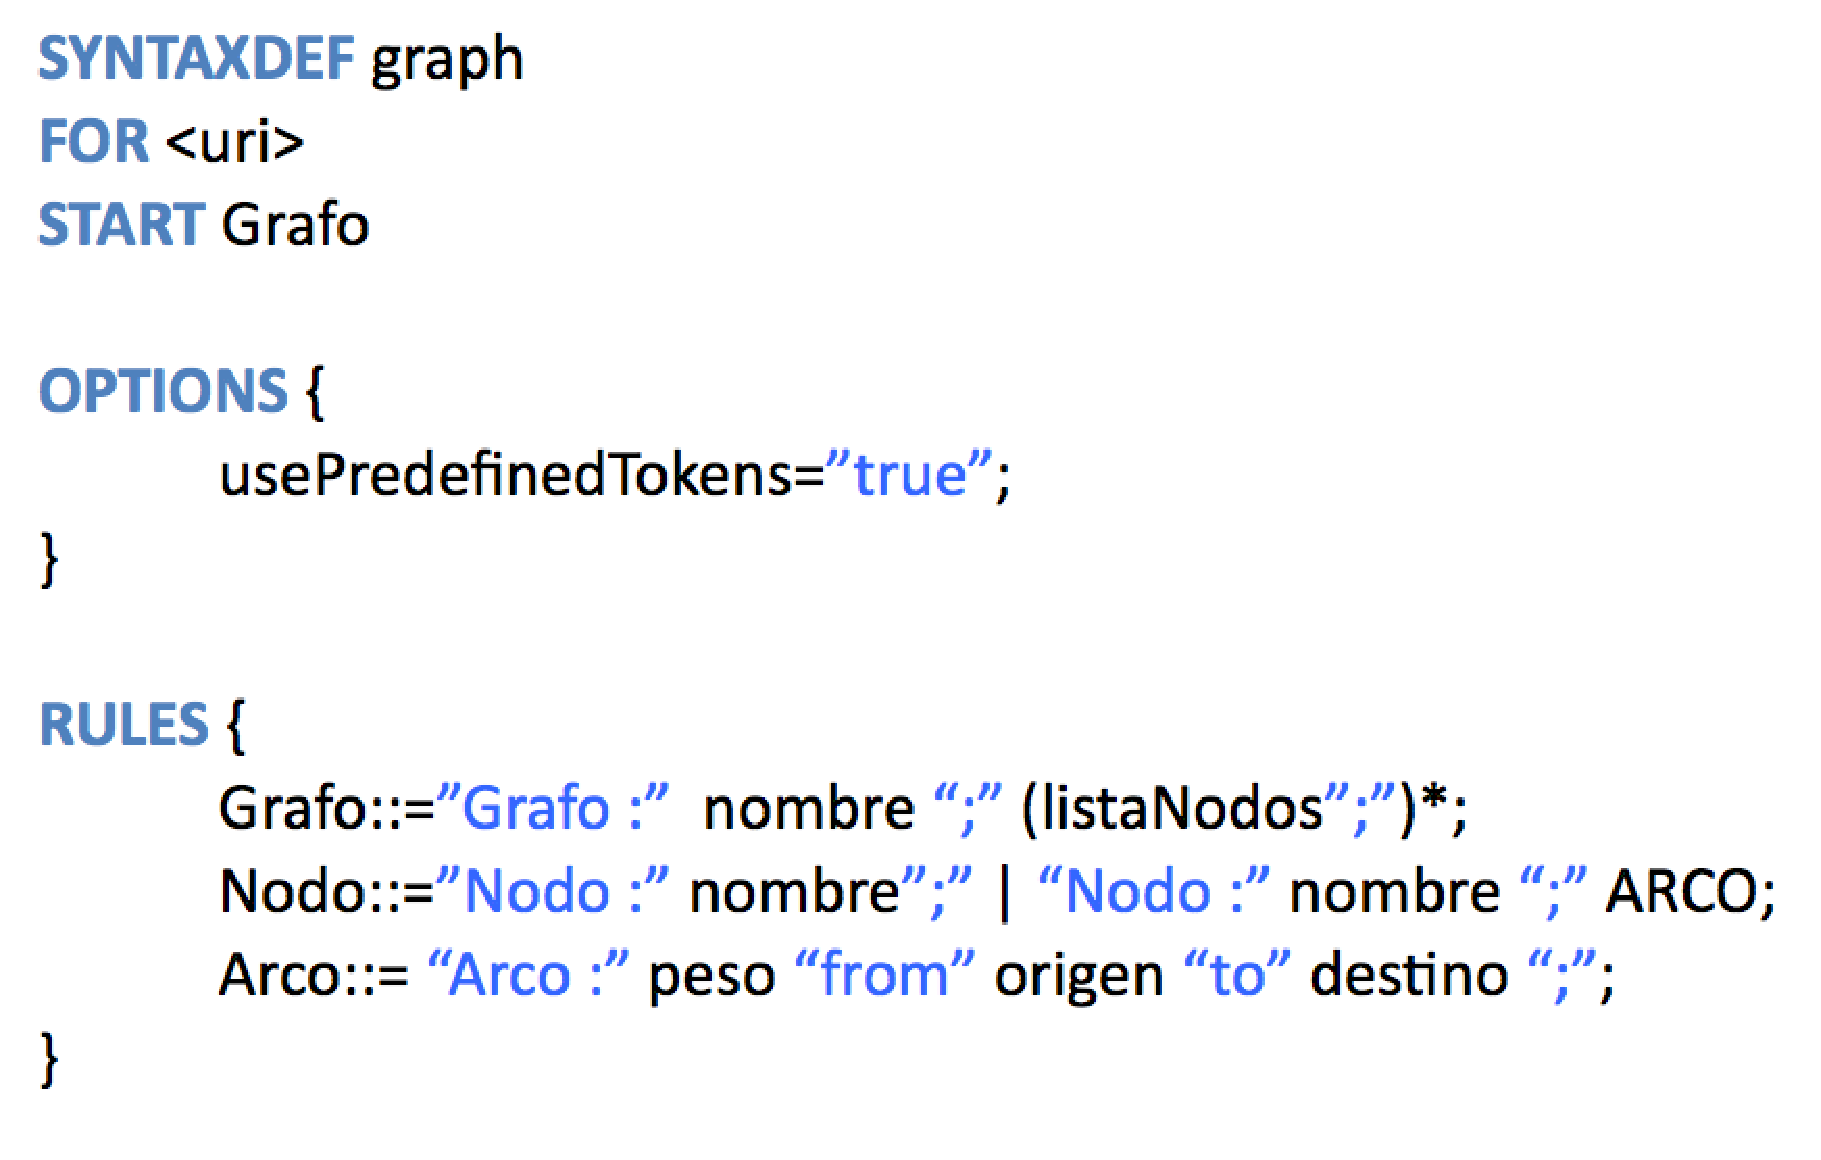
\includegraphics[scale=0.25]{background/gramaticaGrafo.eps}
    \caption{Gram�tica para el ejemplo del lenguaje de los grafos}
    \label{fig:sle:gramaticaGrafos}
\end{figure}

La sintaxis de EMFText difiere de las sintaxis BNF en que existen una serie de directivas para asociar elementos de la sintaxis textual con metaclases, de forma que se generen instancias de dichas metaclases a medida que se procesa el c�digo de un modelo. Por ejemplo, tal y como est� definida la gram�tica de la Figura~\ref{fig:sle:gramaticaGrafos}, a medida que vamos definiendo los arcos estamos indicando la informaci�n tanto de su peso como de sus nodos origen y destino. De este modo, EMFText genera una instanciaci�n de la metaclase Arco que inicializa con los datos le�dos y la a�ade a la instancia global del metamodelo.

La gran ventaja de EMFText es permite generar, a partir de la definici�n de una gram�tica, una gran cantidad de c�digo, liberando al programador de tareas tediosas que adem�s en muchos casos podr�an resultar complicadas. Utilizando EMFText se puede generar autom�ticamente: (1) un editor para nuestro lenguaje, con facilidades como coloreado de la sintaxis o autocompletado; (2) un procesador para el lenguaje capaz de generar una instancia de su correspondiente metamodelo; y (3) el c�digo necesario para empaquetar y distribuir dicho editor como un \emph{plug-in} para Eclipse. Adem�s, todo el c�digo generado es completamente independiente de EMFText, por lo que puede ser ejecutado en plataformas que no tengan instalado dicha herramienta; y es personalizable. Por ejemplo, se puede modificar f�cilmente el postprocesador de nuestra gram�tica. 






\section{Arquitectura de plugins de Eclipse}
\label{sec:back:eplugins}
%%==================================================================%%
%% Author : Tejedo Gonz�lez, Daniel                                 %%
%%          S�nchez Barreiro, Pablo                                 %%
%% Version: 1.0, 18/11/2012                                         %%                   
%% Version: 1.0, 06/02/2013                                         %%                   
%%                                                                  %%
%% Memoria del Proyecto Fin de Carrera                              %%
%% Antecedentes, arquitectura de plugins de eclipse                 %%
%%==================================================================%%

En entorno de desarrollo Eclipse es un ejemplo de arquitectura modular f�cilmente extensible mediante una compleja, pero sencilla al programador, arquitectura de \emph{plug-ins}. Un \emph{plug-in} en Eclipse es un componente que provee un cierto tipo de servicio dentro del contexto del espacio de trabajo de Eclipse. Es decir, una herramienta que se puede integrar en el entorno Eclipse junto con sus otras funcionalidades. Dado que la herramienta \emph{Hydra} fue dise�ada como un \emph{plug-in} para Eclipse, y nuestro editor pretende integrarse tanto en \emph{Hydra} como en \emph{Eclipse}, es necesario conocer y manejar el funcionamiento de la arquitectura de plug-ins de Eclipse.

%%==============================================================================================%%
%% NOTA(Pablo): Esto no se entiende nada
%%==============================================================================================%%
%%
%% En particular, se han utilizado mucho los puntos de extensi�n. Un punto de extensi�n en un
%% plug-in indica la posibilidad de que ese plug-in sea a su vez parte de otro, o que haya 
%% otros plug-ins que sean parte de �l. Esta particularidad permite no s�lo la integraci�n de 
%% nuestro editor con Hydra, sino tambi�n la personalizaci�n de men�s y botones para �l 
%% gracias a la creaci�n de puntos de extensi�n con plug-ins de creaci�n de men�s y barras de
%% herramientas.
%%
%%==============================================================================================%%

%%==============================================================================================%%
%% NOTA(Pablo): Para solucionar
%% - Describir en uno o dos p�rrafos c�mo funciona la arquietctura de plug-ins para Eclipse
%% - Poner un ejemplo de punto de extensi�n, sencillo y concreto, y explicar como funciona 
%%   el punto de extensi�n utilizando algo de c�digo.
%% Si no sabes como escribir esta secci�n, la eliminas directamente, y actualizas la intro 
%% al Cap�tulo de forma conveniente.
%%==============================================================================================%%


\section{Sumario}
\label{sec:back:sumario}
\todo{Escribe un peque�o sumario para el cap�tulo}
% %%==================================================================%%
%% Author : Tejedo Gonz�lez, Daniel                                 %%
%%          S�nchez Barreiro, Pablo                                 %%
%% Version: 1.0, 25/11/2012                                         %%                   
%%                                                                  %%
%% Memoria del Proyecto Fin de Carrera                              %%
%% Sintaxis abstracta, sumario                          %%
%%==================================================================%%

Durante el presente cap�tulo se ha descrito el proceso de definici�n de la sintaxis abstracta de nuestro lenguaje. Este proceso abarca subtareas como la captura de requisitos del lenguaje, la creaci�n de un metamodelo que permita la creaci�n de sintaxis concretas apropiadas, la validaci�n de restricciones externas a ese metamodelo, y las pruebas que corroboren que todos los elementos creados funcionan correctamente. En el siguiente cap�tulo profundizaremos acerca del dise�o de la gram�tica para nuestro lenguaje, as� como de las herramientas utilizadas para implementar esa gram�tica.


% Cap�tulo 3: Creaci�n de la sintaxis abstracta
%%==================================================================%%
%% Author : Tejedo Gonz�lez, Daniel                                 %%
%%          S�nchez Barreiro, Pablo                                 %%
%% Version: 1.0, 25/11/2012                                         %%
%% Version: 2.0, 06/02/2013                                         %%
%%                                                                  %%
%% Memoria del Proyecto Fin de Carrera                              %%
%% Sintaxis abstracta, archivo ra�z                                 %%
%%==================================================================%%

\chapterheader{Desarrollo de la Sintaxis Abstracta}{Desarrollo de la Sintaxis Abstracta}
\label{chap:metamodelo}

El presente cap�tulo describe el proceso de desarrollo de nuestra primera tarea de acuerdo al proceso de desarrollo dirigido por modelos de nuestro lenguaje. Dicha tarea es el desarrollo de un metamodelo o sintaxis abstracta para nuestro lenguaje.

\chaptertoc

\section{Introducci�n}
\label{sec:meta:requisitos}
\todo{Escribir una introducci�n, que es como un mini toc pero con m�s detalle describiendo la estructura de cap�tulo. Al final de la secci�n, describe la estructura del cap�tulo}
%%%==================================================================%%
%% Author : Tejedo Gonz�lez, Daniel                                 %%
%%          S�nchez Barreiro, Pablo                                 %%
%% Version: 1.0, 27/11/2012                                         %%                   
%% Version: 2.0, 09/02/2013                                         %%                   
%%                                                                  %%
%% Memoria del Proyecto Fin de Carrera                              %%
%% Gram�tica, Introducci�n                                                %%
%%==================================================================%%

Siguiendo la metodolog�a impuesta por la Ingenier�a de Lenguajes Dirigida por Modelos, la siguiente parte del desarrollo de nuestro lenguaje pasa por definir la sintaxis concreta textual del mismo. Para poder llevar a cabo esta tarea es necesario escribir una gram�tica, que se encargar� de transformar el c�digo que escribamos en nuestro lenguaje en instancias v�lidas del metamodelo inicial. La captura de requisitos de la gram�tica es pr�cticamente id�ntica a la que se hizo en el cap�tulo anterior para dise�ar el metamodelo, pues en ambos casos es necesario conocer las operaciones del lenguaje y su sintaxis. 

El cap�tulo se estrucurar� del siguiente modo: en primer lugar hablaremos sin entrar en mucho detalle de la herramienta \emph{EMFText}, que es la que hemos escogido para dise�ar nuestra gram�tica. A continuaci�n, y en la misma secci�n, describiremos esta gram�tica y las partes que la componen. Por �ltimo mostraremos las pruebas a las que fue sometida para corroborar que su funcionamiento era el apropiado.

\section{Captura de requisitos}
\label{sec:meta:requisitos}
%%==================================================================%%
%% Author : Tejedo Gonz�lez, Daniel                                 %%
%%          S�nchez Barreiro, Pablo                                 %%
%% Version: 1.0, 25/11/2012                                         %%
%% Version: 2.0, 06/02/2013                                         %%
%%                                                                  %%
%% Memoria del Proyecto Fin de Carrera                              %%
%% Sintaxis abstracta, requisitos                                   %%
%%==================================================================%%

El primer paso para desarrollar nuestro lenguaje era conocer qu� aspecto deb�a tener nuestro lenguaje y qu� restricciones deb�a satisfacer. Es decir, en primer lugar debemos realizar un proceso que podemos denominar de captura de requisitos para poder comprender qu� es lo que tiene que hacer exactamente el lenguaje que se pretende crear.

Concretamente nuestro lenguaje hab�a sido pr�cticamente definido por el profesor Pablo S�nchez, del Departamento de Matem�ticas, Estad�stica y Computaci�n de la Universidad de Cantabria, mediante notaci�n BNF. Dicha gram�tica, se muestra en la Figura~\ref{fig:constraintBNF}. Las ideas subyacentes a dicho lenguaje son las que se describen a continuaci�n. 

\begin{figure}[!tb]
    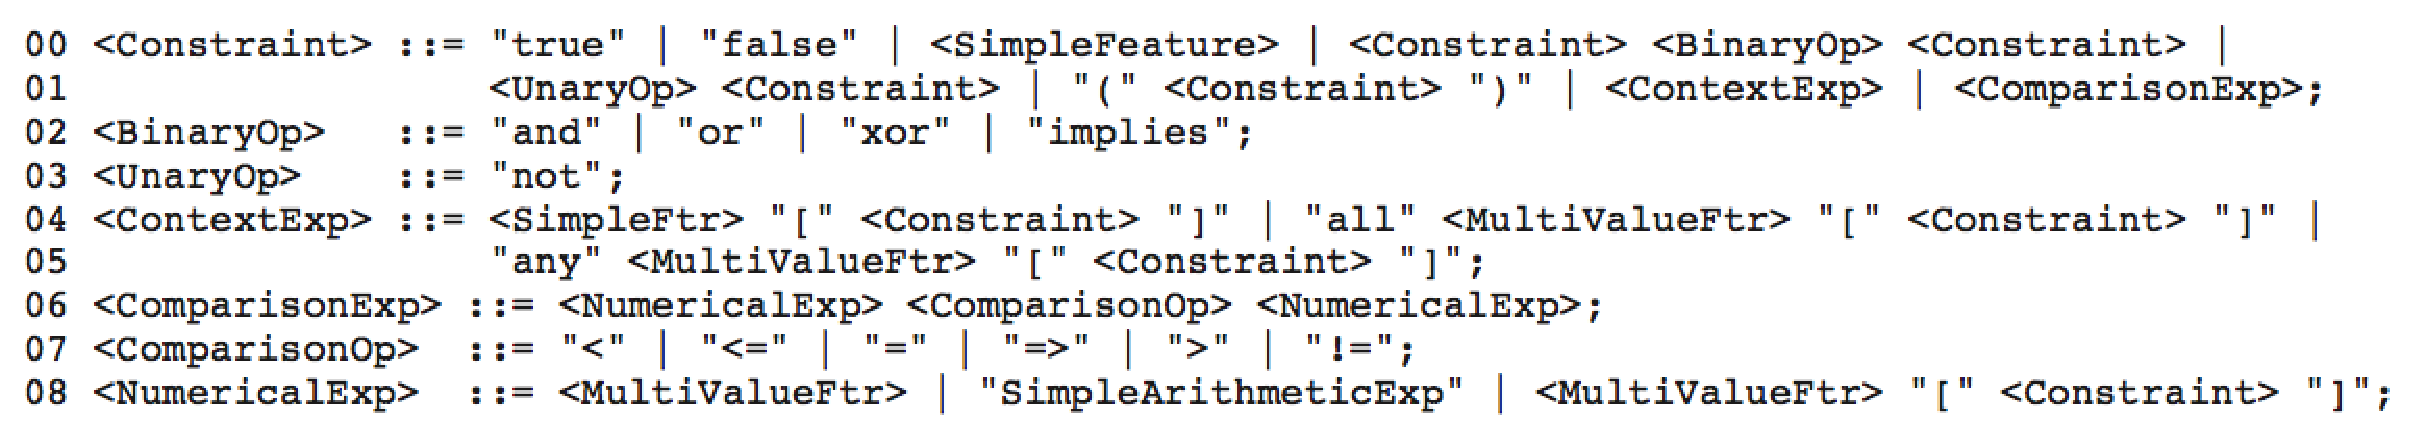
\includegraphics[scale=0.3]{metamodelo/constraintBNF.eps}
    \caption{Gram�tica en notaci�n BNF del lenguaje HCL}
    \label{fig:constraintBNF}
\end{figure}

En dicho lenguaje, una \emph{restricci�n} es una expresi�n l�gica que se puede evaluar a verdadero o falso. Una restricci�n puede ser simplemente un literal, es decir, $true$ o $false$, que se evaluar� a verdadero y falso respectivamente. Una restricci�n tambi�n puede ser una caracter�stica simple, es decir, una caracter�stica que puede aparecer en las configuraciones como m�ximo una vez. Una caracter�stica simple se eval�a a verdadero si ha sido seleccionada, y a falso en caso contrario.

Las caracter�sticas clonables son aquellas que pueden ser seleccionadas m�s de una vez en las configuraciones que construyamos sobre nuestro �rbol de caracter�sticas. Una caracter�stica clonable se eval�an como un n�mero entero positivo, incluido el cero. Ese n�mero representa el n�mero de clones que la caracter�stica posee dentro de una configuraci�n, o dicho de otro modo, el n�mero de veces que ha sido seleccionada. El hecho de que se eval�en como si fueran n�meros permite la inclusi�n de operaciones de comparaci�n entre distintas caracter�sticas clonables. Las operaciones de comparaci�n que se han de implementar son las siguientes: $<$,$<$=,$>$,$>=$,$=$,$!=$. Adem�s, tambi�n se puede utilizar el valor de las caracter�sticas clonables para implementar operaciones aritm�ticas b�sicas, tales como la suma, la resta, la multiplicaci�n y la divisi�n. Estas expresiones a su vez se pueden utilizar como subexpresiones, u operandos, dentro de las operaciones de comparaci�n. Las expresiones de comparaci�n se eval�an a verdadero o falso, y tambi�n pueden ser usadas como subexpresiones para crear expresiones l�gicas m�s complejas.

%%============================================================================%%
%% NOTA(Pablo) : Poner un ejemplo de este tipo de restricciones y explicarlas %%
%%============================================================================%%

Tal y como muestra la Figura~\ref{fig:constraintBNF}, una restricci�n tambi�n puede especificar un contexto concreto en el que poder evaluarla. Esto puede hacerse de varias maneras. Se puede especificar un contexto para una restricci�n poni�ndola entre corchetes y especificando el nombre de una caracter�stica al principio de la expresi�n. La caracter�stica usada como contexto puede ser tanto simple como m�ltiple. En el primer caso, la restricci�n s�lo ser� evaluada en el sub�rbol de la configuraci�n cuya ra�z sea la caracter�stica especificada.

%%============================================================================%%
%% NOTA(Pablo) : Poner un ejemplo y explicarlo                                %%
%%============================================================================%%

En el segundo caso entran en juego los operadores $all$ (para todo) y $any$ (existe). La operaci�n $all$ solo se evaluar� a verdadero si la restricci�n entre corchetes se cumple para todas las instancias de la caracter�stica clonable que act�a como contexto. En caso contrario, la operaci�n se evaluar� a falso. La operaci�n $any$ se evaluar� a verdadero si la restricci�n entre corchetes se cumple al menos una vez para todas las instancia de la caracter�stica clonable que act�a como contexto. Si la restricci�n no se cumple para ninguna de las selecciones, la operaci�n $any$ se evaluar� a falso.

%%============================================================================%%
%% NOTA(Pablo) : Poner un ejemplo y explicarlo                                %%
%%============================================================================%%

Merece la pena se�alar que una caracter�stica puede ser considera simple en un contexto determinado y clonable o m�ltiple en otro. Por ejemplo, la caracter�stica $LightMng$ es clonable en el contexto de $RoomFacilities$, pero simple en el contexto de $GeneralFacilities$. Debido a eso la caracter�stica $LightMng$ no puede ser utilizada sin especificar el contexto en el que est� ubicada, pues podr�a provocar un resultado no esperado o err�neo.

En la restricci�n $any Room[RoomFacilities[LightMng]]$ se pueden apreciar los dos diferentes usos para la operaci�n de contexto. Los corchetes externos indican a la operaci�n any que hay que aplicar la restricci�n a todas las habitaciones. Los corchetes internos indican que la caracter�stica $LightMng$ a la que se est� haciendo referencia es la hija de $RoomFacilities$ y no cualquier otra.

Adem�s nuestro lenguaje deb�a permitir vincular un modelo de caracter�sticas sobre el cual se definir�n un conjunto de restricciones externas. Este modelo se utilizar�, por ejemplo, para comprobar que los s�mbolos que aparecen como nombres de caracter�sticas en las restricciones se refieren a caracter�sticas que realmente existen en el �rbol de caracter�sticas. Por ejemplo, una restricci�n del tipo $AdvancedHeating => Heating$ carecer�a de sentido si algunas de las caracter�sticas $AdvancedHeating$ o $Heating$ no apareciesen en el �rbol de caracter�sticas sobre el cual estamos definiendo restricciones.

%%======================================================================================%%
%% NOTA(Pablo): Esto posiblemente sobre al introducir la traducci�n de la Secci�n III.
%%              Si es as�, eliminarla.
%%              Si los conceptos de restricci�n con contexto y operaci�n cuantificada
%%              no apareciesen, meter esta clasificaci�n pero resumida
%%======================================================================================%%
%%
%% De entre todos esos requisitos b�sicos, es necesario entrar en detalle en el n�mero 3
%% y enumerar la lista de operaciones que pueden ser definidas por nuestro lenguaje. Se
%% pueden clasificar en los siguientes tipos: \\
%%
%% - L�gicas: Son operaciones cuyos operandos han de ser caracter�sticas sin
%%   cardinalidad (tambi�n llamadas caracter�sticas simples), y que se evaluan a
%%   verdadero o falso. Entre las operaciones l�gicas encontramos las cl�sicas not,
%%   and, or, xor e implica.
%%
%% - Num�ricas: Sus operandos han de ser caracter�sticas con cardinalidad (tambi�n
%%   llamadas caracter�sticas m�ltiples) o simplemente n�meros. Su resultado se evalua
%%   con un valor num�rico. Las operaciones num�ricas a implementar son la suma, resta,
%%   multiplicaci�n y divisi�n.
%%
%% - Comparativas: Sus operandos han de ser caracter�sticas m�ltiples o simplemente n�meros,
%%   pero su resultado se evalua con un valor booleano. Las operaciones de comparaci�n a
%%   implementar son igual que, mayor que, menor que, distinto que, mayor o igual que y menor
%%   o igual que.
%%
%% - Operaci�n de contexto: Operaci�n que permite hacer referencia a una caracter�stica
%%   hija de otra caracter�stica. Esta operaci�n tiene sentido para seleccionar
%%   caracter�sticas cuyo nombre pueda estar repetido pero que tengan contextos diferentes.
%%   Por ejemplo, en el modelo de caracter�sticas SmartHome de la figura \ref{figsmarthome}
%%   podemos observar que la caracter�stica HeaterMng est� presente en muchos contextos
%%   diferentes. Esta operaci�n es necesaria para poder saber con seguridad a cual de esos
%%   contextos estamos aplicando la restricci�n.
%%
%% - Operaci�n de selecci�n: Operaci�n que corresponde a los operadores l�gicos cl�sicos
%%   "para todo" o "existe", y que tiene la misma funcionalidad. Evalua si una restricci�n
%%   se cumple para todos los casos en que puede existir  o si se cumple en alguno de los
%%   casos. Por ejemplo, en el modelo de la figura \ref{figsmarthome} se podr�a evaluar una
%%   restricci�n para cada una de las habitaciones que hayan sido definidas, y saber si se
%%  cumple en todas, en alguna o en ninguna.
%%
%%======================================================================================%%

Utilizando esta informaci�n como base, procedimos a crear el correspondiente metamodelo en Ecore para nuestro lenguaje.




\section{Creaci�n del metamodelo}
\label{sec:meta:creacion}
%%==================================================================%%
%% Author : Tejedo Gonz�lez, Daniel                                 %%
%%          S�nchez Barreiro, Pablo                                 %%
%% Version: 1.0, 25/11/2012                                         %%                   
%%                                                                  %%
%% Memoria del Proyecto Fin de Carrera                              %%
%% Sintaxis abstracta, creacion metamodelo                          %%
%%==================================================================%%

Una vez hemos conocidos cu�les son los requisitos que deb�a satisfacer nuestro lenguaje, procedimos a construir un metamodelo en Ecore que cumpla tales requisitos. Dicho metamodelo se muestra en la Figura~\ref{figmetameta}.

%%==================================================================%%
%% NOTA(Pablo): Intenta meter esta figura de forma apaisada         %%
%%              Intenta que la figura se vea menos borrosa.         %%
%%              Intenta que la figura tenga menos cruces de linea   %% 
%%              �Es una captura de pantalla?                        %% 
%%==================================================================%%

\begin{figure}[!tb]
    \centerline{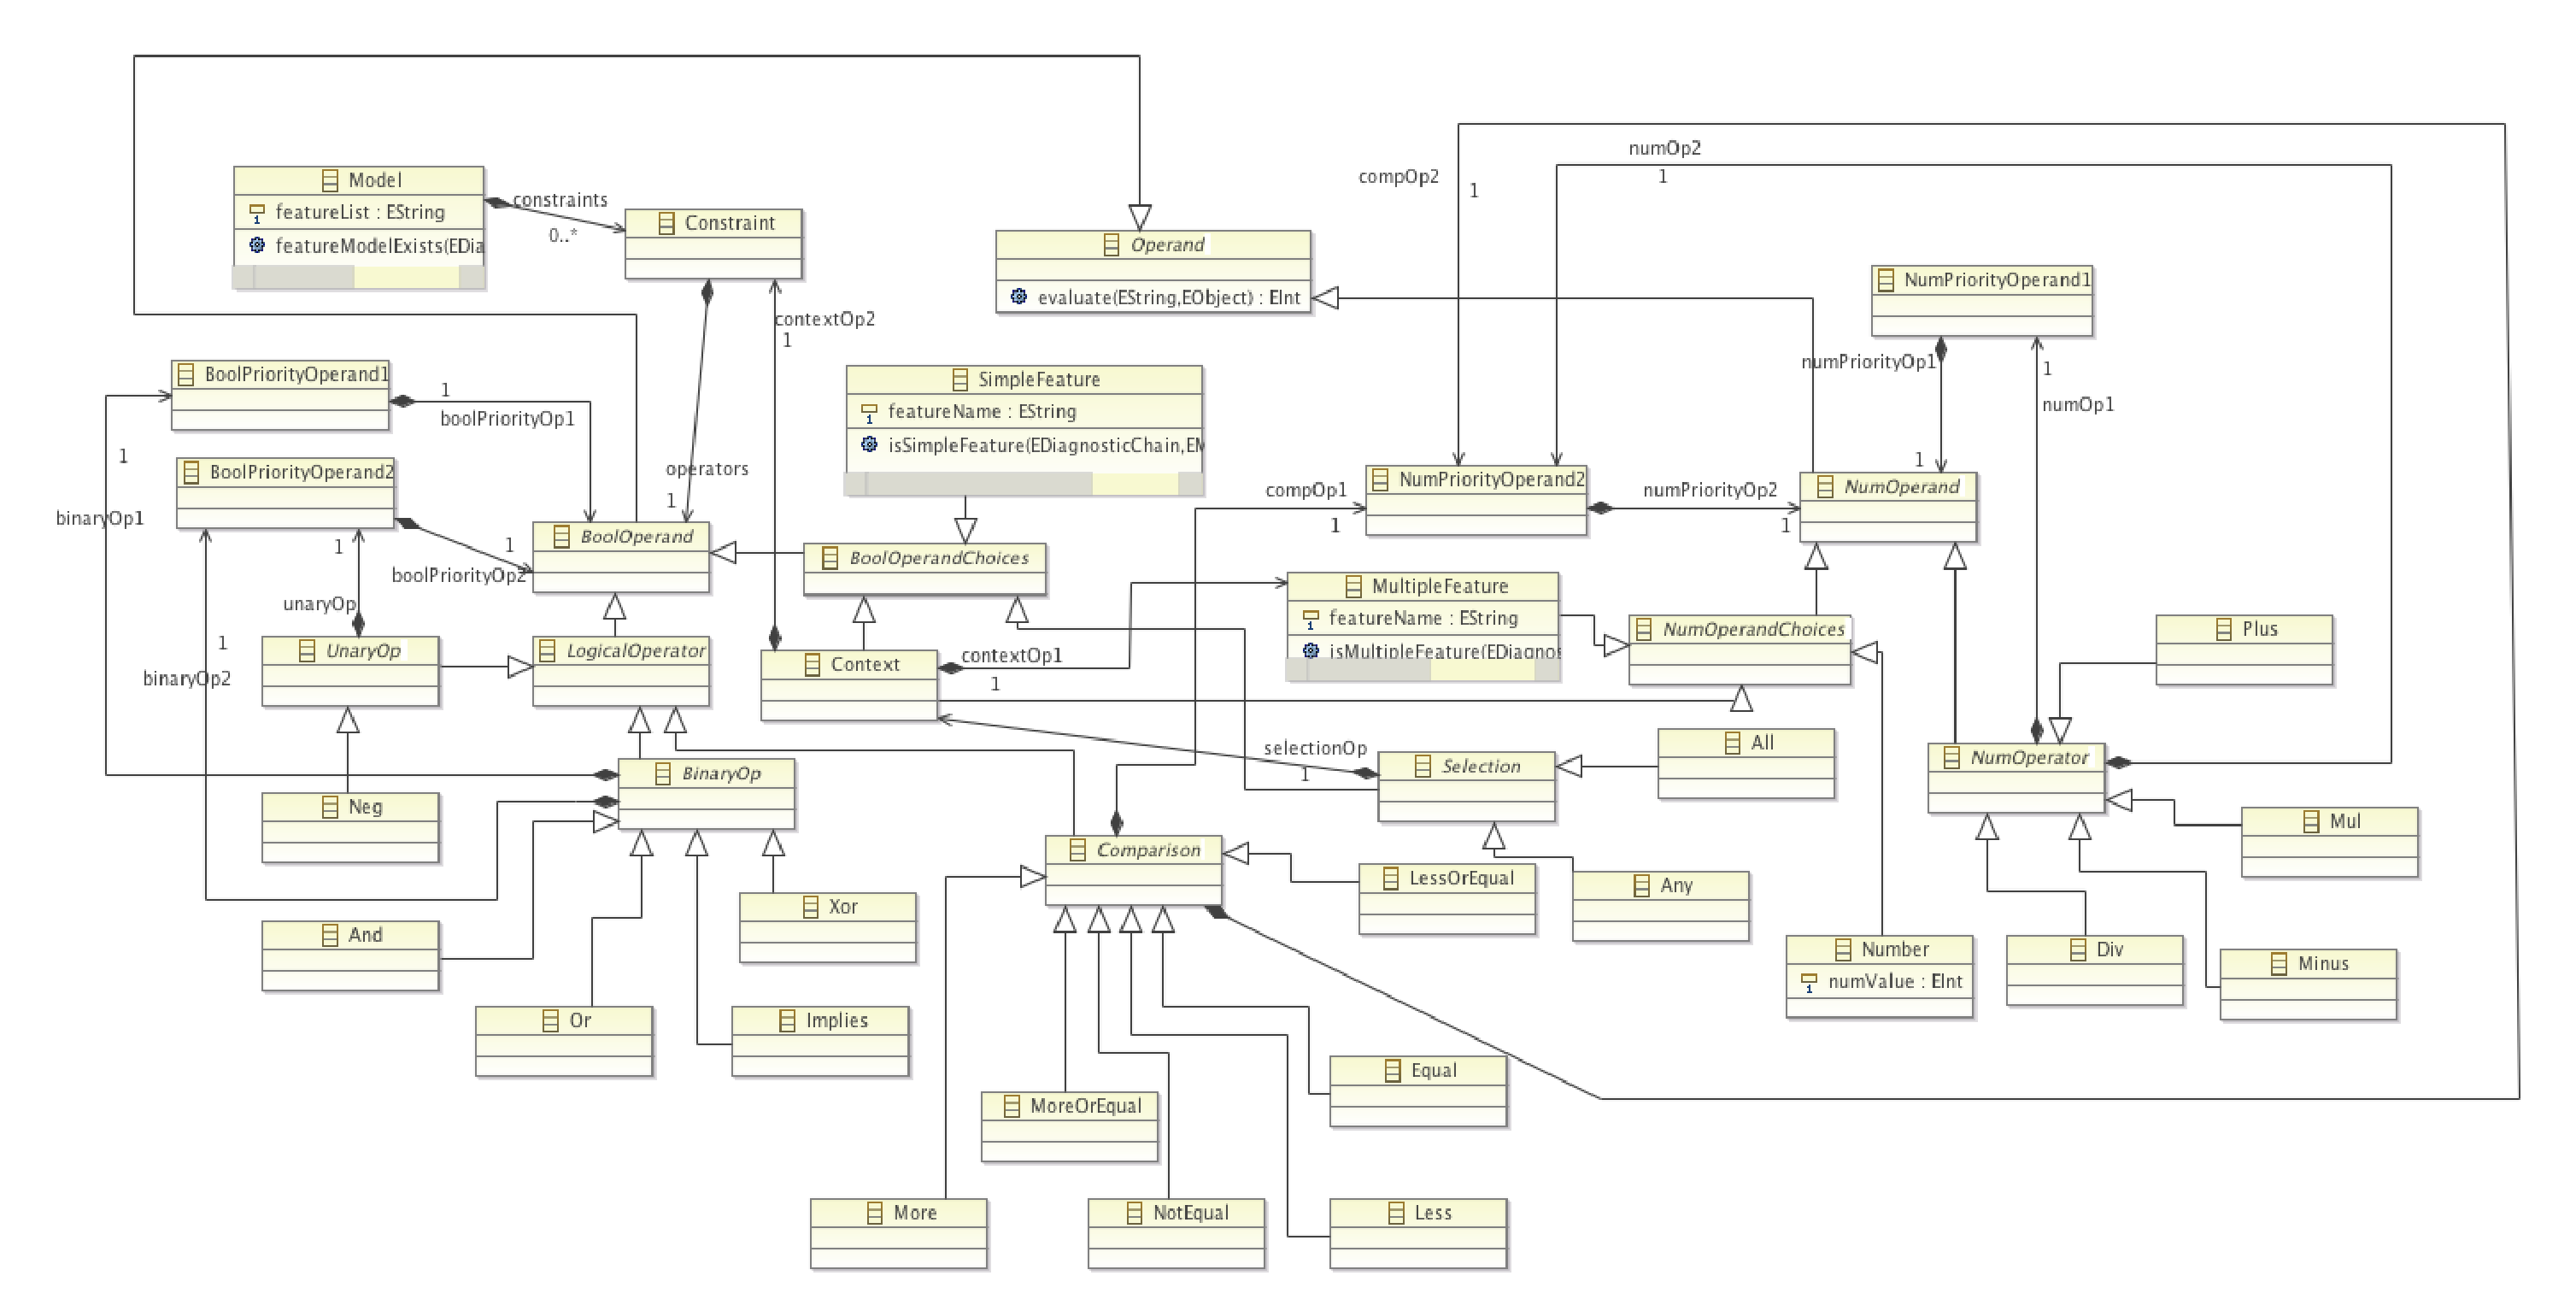
\includegraphics[scale=0.38, angle=90]{metamodelo/metamodelo.eps}}
    \caption{Metamodelo para el lenguaje HCL}
    \label{figmetameta}
\end{figure}

La clase \emph{Model} es la que sirve de punto de entrada y contender para el resto de las clases de nuestro metamodelo. 

C�mo se ha comentado anteriormente, debemos vincular un conjunto de restricciones con el �rbol de caracter�sticas al cual deben aplicarse. Dicho �rbol de caracter�sticas debe haber sido previamente creado usando la herramienta \emph{Hydra}, de acuerdo con los objetivos generales del proyecto. Eso reduce mucho el n�mero de factores de los que hay preocuparse, vi�ndose reducidos en este punto a tener que almacenar �nicamente la localizaci�n del fichero que contiene dicho �rbol de caracter�stica, con objeto de poder cargarlo cuando se necesite. La ruta de dicho fichero se almacena en el atributo \emph{featureList} de la clase \emph{Model}.

Un modelo de restricciones permite especificar un n�mero indeterminado de restricciones, representadas por la clase \emph{Constraint}. Por tanto, la clase \emph{Model} contendr� 0 o m�s restricciones (en principio se permiten definir ficheros sin restricciones, que se entiende se refinar�n postriormente). 

Una restricci�n es una expresi�n booleana que se eval�a a vedadero o falso, y que contendr� un operador booleano, representando por la clase \emph{BoolOperand}, y varios operadores, representados por diversas clases. 

Un operador booleano puede ser tanto una \emph{SimpleFeature}, es decir, una caracter�stica no clonable, como una operaci�n cuya evaluaci�n de como resultado un valor booleano. Estas operaciones pueden ser l�gicas (\emph{and}, \emph{or}, \emph{implies}, \emph{xor} y \emph{not}), de comparaci�n ($<$, $<=$, $>$, $>=$, =, !=), de selecci�n (\emph{all} y \emph{any}) o de contexto.

Por otro lado, una restricci�n tambi�n puede contener operadores num�ricos. Un operador num�rico puede ser una \emph{MultipleFeature}, es decir, una caracter�stica clonable, un n�mero, o una operaci�n cuya evaluaci�n de como resultado un valor num�rico. Estas operaciones son artim�ticas, es decir, $+$, $-$, $*$ y $/$. El operador m�s prioritario de una restricci�n siempre ha de ser booleano, pues en �ltima instancia esta tiene que poder ser evaluada a verdadero o falso.

Las operaciones l�gicas y num�ricas descritas est�n representadas en el metamodelo mediante las metaclases que llevan su nombre. Es decir, \emph{LessOrEqual} es la operaci�n $<=$, \emph{Plus} es la operaci�n $+$, y as� sucesivamente. Se puede apreciar que estas metaclases son las hojas de una estructura de herencias. Esta estructura permite no solo facilitar la comprensi�n del metamodelo, sino tambi�n servir de apoyo a \emph{EMFText} en el momento de construir la posterior gram�tica. 

Como ejemplo, vamos a seguir esta estructura a trav�s de una de las operaciones, \emph{Implies}. Esta metaclase hereda de \emph{BinaryOp}, que es la metaclase que representa las operaciones l�gicas con dos operandos. \emph{BinaryOp} a su vez hereda de \emph{LogicalOperator}, que representa las operaciones l�gicas. Por �ltimo, \emph{LogicalOperator} hereda de \emph{BoolOperand}, que representa los operadores booleanos. Un an�lisis an�logo se podr�a realizar con cualquiera de las operaciones implementadas.

Cabe tambi�n mencionar algunas metaclases como \emph{BoolPriorityOperand1} que parecen ajenas a esta estructura y cuya presencia puede resultar dudosa. Su inclusi�n se justifica por razones de funcionamiento de la herramienta \emph{EMFText}, que requiere un tratamiento especial a la hora de implementar prioridad entre las operaciones.

Los atributos de las metaclases sirven para almacenar informaci�n importante para el lenguaje, que posteriormente podr�a ser utilizada a nivel de validaci�n o ejecuci�n. De estos atributos ya se ha mencionado la utilidad de \emph{featureList}, dentro de la clase \emph{Model}. Adem�s de este, el atributo \emph{featureName} de las clases \emph{SimpleFeature} y \emph{MultipleFeature} sirve para almacenar el nombre de la caracter�stica a la que hagan alusi�n. Por �ltimo, el atributo \emph{numValue} de la clase \emph{Number} sirve para guardar el valor literal num�rico que haya sido introducido.

%\todo{sigue t� describiendo el metamodel o en este estilo, describiendo su estructura sin entrar en detalles ni ponerte demasiado barroco. Describes lo que hay, no el proceso de c�mo lo hiciste ni si te cost� m�s o menos, o te pareci� f�cil o dificil. No describas las asociaciones entre metaclases, eso es demasiado detalle}.

%%========================================================================================%%
%% NOTA(Pablo): Todo lo de abajo quedar� redundante con el nuevo texto, as� que mejor     %%
%%              eliminarlo                                                                %% 
%%========================================================================================%%

%%========================================================================================%%
%% INICIO DE PARTE POSIBLEMENTE REDUNDANTE                                                %%
%%========================================================================================%%

%El primer paso es definir toda la estructura necesaria para la implementaci�n de las operaciones, haciendo que cada una de ellas est� representada en nuestro metamodelo mediante una clase, pero sin preocuparnos todav�a por las relaciones entre ellas. La clase ra�z de toda esta estructura es Operand. Es una clase abstracta, es decir, en los modelos que luego instanciemos de este metamodelo no podr� haber ninguna instancia de Operand, s�lo de los hijos no abstractos que tenga. A medida que vayamos definiendo clases hijas  de Operand estaremos especificando cada vez con m�s exactitud a qu� tipo de operaci�n estamos haciendo referencia.
%
%En el segundo nivel de la estructura de implementaci�n de las operaciones hacemos una ramificaci�n seg�n el tipo del valor de retorno o de evaluaci�n de las posibilidades. Es decir, a la clase Operand le a�adiremos dos hijos: BoolOperand para operaciones que se eval�an a booleano y NumOperand para operaciones que se eval�an a num�rico. Estas clases tambi�n ser�n abstractas.
%
%El proceso de divisi�n a partir de aqu� es m�s o menos an�logo para todas las operaciones, as� que vamos a centrarnos �nicamente en la rama que da lugar a las operaciones binarias l�gicas, para comentar despu�s los casos y situaciones especiales. Una vez tenemos la clase BoolOperand, podemos especializarla un poco m�s a LogicalOperator, que a su vez se dividir� en operaciones unarias, binarias, o de comparaci�n. Todas ellas son clases abstractas. Por fin, la clase BinaryOp heredar� las clases de las operaciones propiamente dichas, en este caso And, Or, Implies y Xor. Estas ya podr�n ser instanciadas en las sintaxis concretas que creemos.
%
%Cabe hacer menci�n tambi�n a las clases SimpleFeature, MultipleFeature y Number, que representan a las caracter�sticas simples, m�ltiples y n�meros respectivamente. En cualquier �rbol resultante de parsear nuestro lenguaje, estas clases representar�n las hojas. En �ltima instancia todas las operaciones tendr�n como operandos caracter�sticas o n�meros. Podemos observar que SimpleFeature es un operando booleano (est� en la parte estructural de las operaciones booleanas) ya que su evaluaci�n ser� verdadero o falso, dependiendo si esa caracter�stica ha sido seleccionada en la configuraci�n correspondiente o no. MultipleFeature sin embargo se eval�a a n�mero entero. Su valor ser� el n�mero de apariciones de esa caracter�stica dentro de la configuraci�n correspondiente.
%
%Muchas de las clases que ahora se pueden contemplar en el metamodelo de la figura \ref{figmetameta} a�n no estaban presentes en esta etapa temprana del dise�o, y su inclusi�n fue necesaria a ra�z de la creaci�n de la gram�tica y los problemas que se observaron en ese punto. En particular, las terminadas en Choices y en PriorityOperand. Las operaciones All, Any y Context en este momento eran simples herencias de BoolOperand. El motivo de estas modificaciones ser� explicado en el cap�tulo siguiente.
%
%Para terminar este apartado, vamos a hablar de las relaciones entre las diferentes clases de nuestro metamodelo. En este punto del dise�o no eran las mismas que las de la figura \ref{figmetameta} por los motivos explicados anteriormente. Simplemente busc�bamos una forma de relacionar cada operaci�n con los tipos de sus operandos (que tambi�n pueden ser operaciones, como es l�gico). Las operaciones l�gicas binarias tendr�n dos operandos que tambi�n ser�n binarios. En este momento del dise�o binaryOp1 y binaryOp2 iban relacionados a BoolOperand, al igual que unaryOp. Del mismo modo, compOp1, compOp2, numOp1 y numOp2 (es decir, los operandos de operaciones de comparaci�n y num�ricas respectivamente) estaban relacionados con la clase NumOperand.
%
%La relaci�n de toda estructura de operaciones con los dos elementos anteriores, Model y Constraint, se realiza entre Constraint y BoolOperand. Toda restricci�n en �ltima ha de ser evaluada a verdadero o falso, es por eso que la relaci�n no va con Operand, como podr�a pensarse en primera instancia. De este modo estamos forzando que la operaci�n con menos profundidad del �rbol parseado de nuestra restricci�n sea booleana, y que por lo tanto el resultado final de validar la restricci�n sea un dato booleano.
%
%Quiz�s a alguien le pueda sorprender el hecho de que la relaci�n ''operators'' entre Constrain y BoolOperand sea 1..1 y no 1..*. El motivo es que como los operadores de esa primera operaci�n booleana que estamos forzando pueden ser a su vez operaciones, la complejidad en la restricci�n que podemos definir se propaga por ah� en lugar de por la relaci�n creada.

%%========================================================================================%%
%% FIN DE PARTE POSIBLEMENTE REDUNDANTE                                                   %%
%%========================================================================================%%

Como se coment� en la Secci�n~\ref{sec:intr:sle}, no todas las restricciones que debe satisfacer un lenguaje pueden especificarse mediante la notaci�n propia de un languaje de metamodelado. Para especificar dichas restricciones, se utilizan lenguajes complementarios al lenguaje propio de metamodelado. La siguiente secci�n explica como se definen dichas restricciones para nuestro lenguaje utilizando el EMF Validation Framework.




\section{Especificaci�n de Restricciones Externas}
\label{sec:emfvf:req}
%%==================================================================%%
%% Author : Tejedo Gonz�lez, Daniel                                 %%
%%          S�nchez Barreiro, Pablo                                 %%
%% Version: 1.0, 28/11/2012                                         %%
%% Version: 2.0, 06/02/2013                                         %%
%%                                                                  %%
%% Memoria del Proyecto Fin de Carrera                              %%
%% Validation Framework, implementacion                             %%
%%==================================================================%%

La sintaxis propia de Ecore no nos permite especificar ciertas restricciones que debe satisfacer nuestro metamodelo. Dichas restricciones, las cuales se enumeran a continuaci�n, deben comprobar que:

\begin{enumerate}
    \item La ruta que indica donde est� el �rbol de caracter�sticas al que se
        aplican las restricciones definidas es correctas. Ello implica comprobar tanto que la ruta es correcta como que el fichero que se halla en dicha ruta corresponde de verdad a un �rbol de caracter�sticas.
    \item El atributo \emph{featureName} asociado a una \emph{SimpleFeature} o a una \emph{MultipleFeature} corresponde al nombre de una caracter�stica perteneciente al �rbol de caracter�sticas referenciado.
    \item Una caracter�stica identificada como \emph{SimpleFeature} en el modelo de restricciones (eval�a a verdadero o falso) es realmente una caracter�stica simple (no clonable) en el �rbol de caracter�sticas asociado. Sin esta comprobaci�n, podr�amos, por ejemplo, introducir caracter�sticas m�ltiples como operandos de operadores booleanas como \emph{and} u \emph{or}. En ese caso, ser�a imposible evaluar dichas operaciones ya que no podemos evaluar sus operandos a verdadero o falso.
\end{enumerate}

Respecto a la segunda restricci�n, merece la pena aclarar que el caso contrario, comprobar que una caracter�sticas considerada como m�ltiple en una restricci�n realmente lo sea, no es necesario controlarlo. La raz�n es que las caracter�sticas simples pueden tratarse como un caso particular o subtipo de caracter�stica m�ltiples, ya que siempre podremos considerarla como una caracter�stica clonable con cardinalidad $<0,1>$.

Para implementar estas restricciones externas se ha utilizado \emph{EMF Validation Framework}, herramienta integrada en EMF para este prop�sito concreto. Siguiendo las instrucciones proporcionadas por esta herramienta, a�adimos un m�todo de validaci�n a cada metaclase que necesitaba ser validada. En nuestro caso, dichas clases eran \emph{Model}, \emph{SimpleFeature} y \emph{MultipleFeature}. De acuerdo con las normas establecida por \emph{EMF Validation Framework}, dichos m�todos deben poseer un perfil concreto. Dicho perfil est� compuesto por dos par�metros, uno llamado \emph{diagnostics} del tipo \emph{EDiagnosticChain} y otro llamado \emph{context} que es un mapa \todo{cual es la clave y cual es valor de este mapa?}. Los m�todos de validaci�n han de retornar siempre un valor booleano.

Si la validaci�n es satisfactoria, el m�todo debe obviamente devolver un valor verdadero. En caso contrario, retornar� falso. El par�metro \emph{diagnostics} es un par�metro de salida que almacena informaci�n sobre el resultado de la validaci�n, tal como el tipo de error producido o el mensaje de error que queremos mostrar al usuario.

%%==========================================================================================%%
%% NOTA(Pablo): Explicar para qu� sirve el mapa                                             %%
%%==========================================================================================%%

Para implementar la primera restricci�n de las comentadas anteriormente, validar que la ruta que indica el �rbol de caracter�sticas sea v�lida y apunte realmente a un �rbol de caracter�sticas, se a�adi� un m�todo de validaci�n a la clase \emph{Model}. Para llevar a cabo esta validaci�n simplemente se carga el fichero existente en la direcci�n indicada y se controla las posibles excepciones que una direcci�n err�nea pueda generar. Adem�s, se comprueba que el contenido de esa direcci�n sea un �rbol de caracter�sticas. Se aprovecha tambi�n para generar una variable global que contenga el modelo le�do, ya que ser� necesario volver a cargarlo en posteriores comprobaciones.

Para implementar la segunda restricci�n, comprobar que la existencia de las caracter�sticas escritas en nuestro fichero de restricciones en el �rbol de caracter�sticas anteriormente asociado, a�adimos m�todos de validaci�n a las metaclases \emph{MultipleFeature} y \emph{SimpleFeature}. Para ello simplemente buscamos que el nombre almacenado en el par�metro \emph{featureName} de dichas metaclases corresponda con el nombre de alguna caracter�sticas del modelo cargado anteriormente. 

Para implementar la segunda restricci�n, que las caracter�sticas identificadas como simples realmente sean realmente simples en el �rbol de caracter�sticas asociado, a�adimos un m�todo de validaci�n a la clase \emph{SimpleFeature}. Para realizar la comprobaci�n tenemos que corroborar que �sta no pueda ser instanciada en m�s de una ocasi�n. Para ello tenemos que calcular la cota superior de su cardinalidad. Si dicha cota fuese mayor que uno, no ser�a una caracter�sticas simple. Este l�mite puede ser superior a uno en el caso de las caracter�sticas clonables, o de la caracter�sticas hijas de caracter�sticas m�ltiples. 

Tras a�adir estas restricciones estaba definida la sintaxis abstracta para nuestro lenguaje. Antes de proceder a la definici�n de una sintaxis concreta para dicho lenguaje, realizamos una serie de pruebas destinadas a verificar que el metamodelo creado recoge la sintaxis abstracta deseada. 


\section{Testeo de la Sintaxis Abstracta}
\label{sec:meta:pruebas}
%%==================================================================%%
%% Author : Tejedo Gonz�lez, Daniel                                 %%
%%          S�nchez Barreiro, Pablo                                 %%
%% Version: 1.0, 25/11/2012                                         %%
%% Version: 1.0, 06/02/2013                                         %%
%%                                                                  %%
%% Memoria del Proyecto Fin de Carrera                              %%
%% Sintaxis abstracta,  pruebas                                     %%
%%==================================================================%%

Una vez creado nuestro metamodelo, deb�amos probar que dicho metamodelo era correcto. Es decir, que permit�a especificar todas las restricciones que dese�bamos crear, a la vez que, por construcci�n, imped�a la especificaci�n de restricciones que deb�an ser consideradas como sint�cticamente incorrectas.

Para ello realizamos una serie de pruebas consistentes en la creaci�n de varias instancias del metamodelo y observar el �rbol de sintaxis abstracta generado, comprobando si �ste se correspond�a con el esperado.

\begin{figure}[t]
    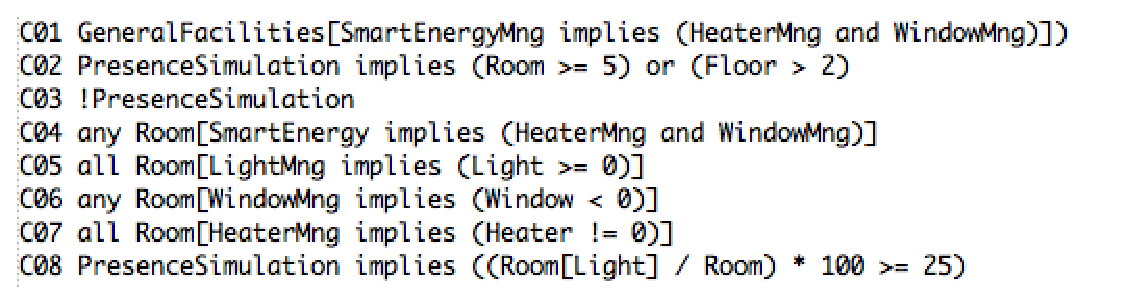
\includegraphics[scale=0.6]{metamodelo/instpruebas.eps}
    \caption{Conjunto de instrucciones que puso a prueba el funcionamiento del metamodelo}
    \label{figmetains}
\end{figure}

Las instrucciones que fueron puestas a prueba fueron las que se ven en la Figura~\ref{figmetains}. Este conjunto de instrucciones servir�n como pruebas tambi�n en momentos m�s avanzados del desarrollo. Dicho conjunto de pruebas fue dise�ado para recoger de la forma m�s exhaustiva posible todas las combinaciones de metaclases posibles.


\section{Sumario}
\label{sec:meta:sumario}


% Cap�tulo 4: Creacion de la gramatica
%%==================================================================%%
%% Author : Tejedo Gonz�lez, Daniel                                 %%
%%          S�nchez Barreiro, Pablo                                 %%
%% Version: 1.0, 27/11/2012                                         %%                   %%                                                                  %%
%% Memoria del Proyecto Fin de Carrera                              %%
%% Gram�tica,  archivo raiz                                       %%
%%==================================================================%%

\chapterheader{Creaci�n de la gram�tica}{Creaci�n de la gram�tica}
\label{chap:gramatica}

Una vez ha sido definido el metamodelo, el siguiente paso es definir la sintaxis concreta textual de nuestro lenguaje, es decir, los medios que permitan expresarnos en �l de modo escrito. De no hacerlo, solo podr�amos usar este lenguaje creando instancias del metamodelo, lo cual l�gicamente no es ni c�modo ni conveniente. Este cap�tulo versa sobre la creaci�n de la gram�tica que permite definir esa sintaxis textual, as� como de las repercusiones que su dise�o tuvo en la sintaxis abstracta.

\chaptertoc

\section{Captura de requisitos}
\label{sec:gram:requisitos}
%%==================================================================%%
%% Author : Tejedo Gonz�lez, Daniel                                 %%
%%          S�nchez Barreiro, Pablo                                 %%
%% Version: 1.0, 25/11/2012                                         %%
%% Version: 2.0, 06/02/2013                                         %%
%%                                                                  %%
%% Memoria del Proyecto Fin de Carrera                              %%
%% Sintaxis abstracta, requisitos                                   %%
%%==================================================================%%

El primer paso para desarrollar nuestro lenguaje era conocer qu� aspecto deb�a tener nuestro lenguaje y qu� restricciones deb�a satisfacer. Es decir, en primer lugar debemos realizar un proceso que podemos denominar de captura de requisitos para poder comprender qu� es lo que tiene que hacer exactamente el lenguaje que se pretende crear.

Concretamente nuestro lenguaje hab�a sido pr�cticamente definido por el profesor Pablo S�nchez, del Departamento de Matem�ticas, Estad�stica y Computaci�n de la Universidad de Cantabria, mediante notaci�n BNF. Dicha gram�tica, se muestra en la Figura~\ref{fig:constraintBNF}. Las ideas subyacentes a dicho lenguaje son las que se describen a continuaci�n. 

\begin{figure}[!tb]
    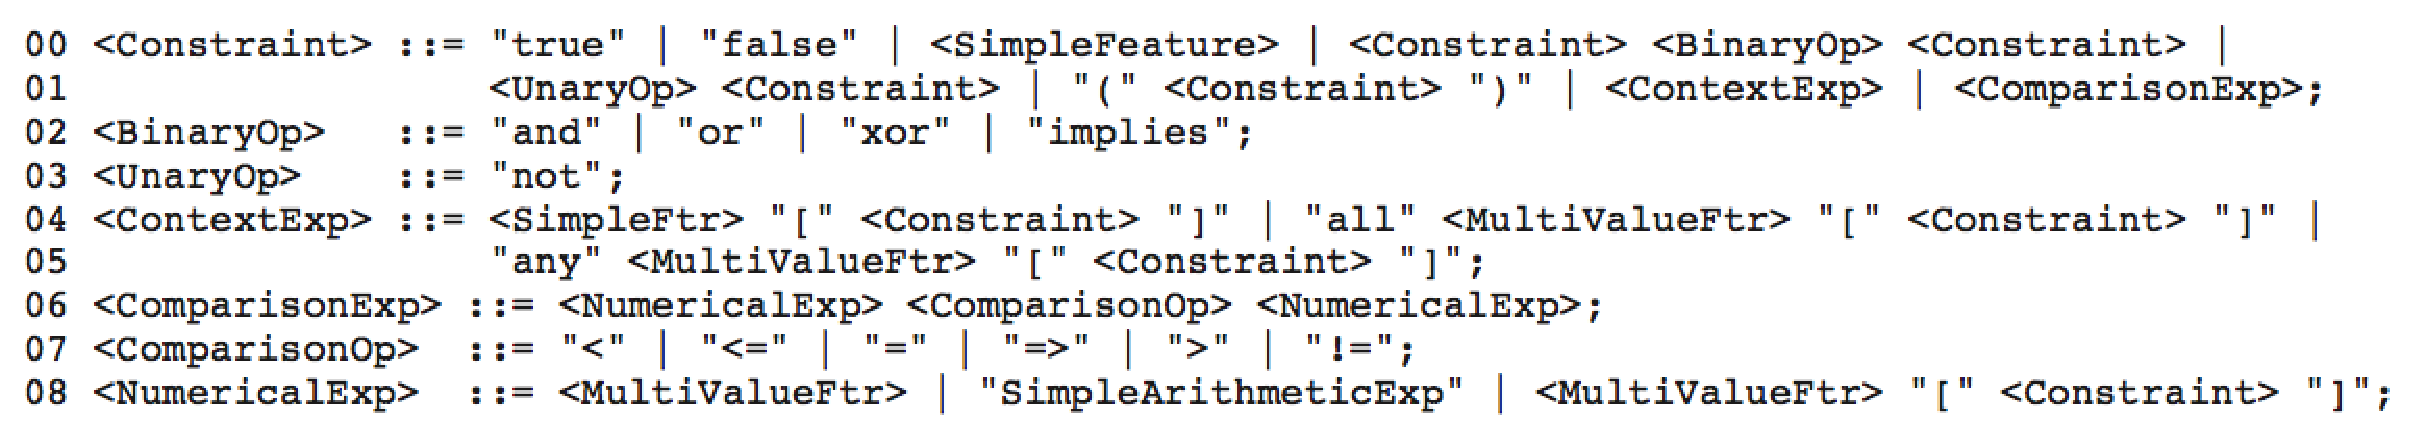
\includegraphics[scale=0.3]{metamodelo/constraintBNF.eps}
    \caption{Gram�tica en notaci�n BNF del lenguaje HCL}
    \label{fig:constraintBNF}
\end{figure}

En dicho lenguaje, una \emph{restricci�n} es una expresi�n l�gica que se puede evaluar a verdadero o falso. Una restricci�n puede ser simplemente un literal, es decir, $true$ o $false$, que se evaluar� a verdadero y falso respectivamente. Una restricci�n tambi�n puede ser una caracter�stica simple, es decir, una caracter�stica que puede aparecer en las configuraciones como m�ximo una vez. Una caracter�stica simple se eval�a a verdadero si ha sido seleccionada, y a falso en caso contrario.

Las caracter�sticas clonables son aquellas que pueden ser seleccionadas m�s de una vez en las configuraciones que construyamos sobre nuestro �rbol de caracter�sticas. Una caracter�stica clonable se eval�an como un n�mero entero positivo, incluido el cero. Ese n�mero representa el n�mero de clones que la caracter�stica posee dentro de una configuraci�n, o dicho de otro modo, el n�mero de veces que ha sido seleccionada. El hecho de que se eval�en como si fueran n�meros permite la inclusi�n de operaciones de comparaci�n entre distintas caracter�sticas clonables. Las operaciones de comparaci�n que se han de implementar son las siguientes: $<$,$<$=,$>$,$>=$,$=$,$!=$. Adem�s, tambi�n se puede utilizar el valor de las caracter�sticas clonables para implementar operaciones aritm�ticas b�sicas, tales como la suma, la resta, la multiplicaci�n y la divisi�n. Estas expresiones a su vez se pueden utilizar como subexpresiones, u operandos, dentro de las operaciones de comparaci�n. Las expresiones de comparaci�n se eval�an a verdadero o falso, y tambi�n pueden ser usadas como subexpresiones para crear expresiones l�gicas m�s complejas.

%%============================================================================%%
%% NOTA(Pablo) : Poner un ejemplo de este tipo de restricciones y explicarlas %%
%%============================================================================%%

Tal y como muestra la Figura~\ref{fig:constraintBNF}, una restricci�n tambi�n puede especificar un contexto concreto en el que poder evaluarla. Esto puede hacerse de varias maneras. Se puede especificar un contexto para una restricci�n poni�ndola entre corchetes y especificando el nombre de una caracter�stica al principio de la expresi�n. La caracter�stica usada como contexto puede ser tanto simple como m�ltiple. En el primer caso, la restricci�n s�lo ser� evaluada en el sub�rbol de la configuraci�n cuya ra�z sea la caracter�stica especificada.

%%============================================================================%%
%% NOTA(Pablo) : Poner un ejemplo y explicarlo                                %%
%%============================================================================%%

En el segundo caso entran en juego los operadores $all$ (para todo) y $any$ (existe). La operaci�n $all$ solo se evaluar� a verdadero si la restricci�n entre corchetes se cumple para todas las instancias de la caracter�stica clonable que act�a como contexto. En caso contrario, la operaci�n se evaluar� a falso. La operaci�n $any$ se evaluar� a verdadero si la restricci�n entre corchetes se cumple al menos una vez para todas las instancia de la caracter�stica clonable que act�a como contexto. Si la restricci�n no se cumple para ninguna de las selecciones, la operaci�n $any$ se evaluar� a falso.

%%============================================================================%%
%% NOTA(Pablo) : Poner un ejemplo y explicarlo                                %%
%%============================================================================%%

Merece la pena se�alar que una caracter�stica puede ser considera simple en un contexto determinado y clonable o m�ltiple en otro. Por ejemplo, la caracter�stica $LightMng$ es clonable en el contexto de $RoomFacilities$, pero simple en el contexto de $GeneralFacilities$. Debido a eso la caracter�stica $LightMng$ no puede ser utilizada sin especificar el contexto en el que est� ubicada, pues podr�a provocar un resultado no esperado o err�neo.

En la restricci�n $any Room[RoomFacilities[LightMng]]$ se pueden apreciar los dos diferentes usos para la operaci�n de contexto. Los corchetes externos indican a la operaci�n any que hay que aplicar la restricci�n a todas las habitaciones. Los corchetes internos indican que la caracter�stica $LightMng$ a la que se est� haciendo referencia es la hija de $RoomFacilities$ y no cualquier otra.

Adem�s nuestro lenguaje deb�a permitir vincular un modelo de caracter�sticas sobre el cual se definir�n un conjunto de restricciones externas. Este modelo se utilizar�, por ejemplo, para comprobar que los s�mbolos que aparecen como nombres de caracter�sticas en las restricciones se refieren a caracter�sticas que realmente existen en el �rbol de caracter�sticas. Por ejemplo, una restricci�n del tipo $AdvancedHeating => Heating$ carecer�a de sentido si algunas de las caracter�sticas $AdvancedHeating$ o $Heating$ no apareciesen en el �rbol de caracter�sticas sobre el cual estamos definiendo restricciones.

%%======================================================================================%%
%% NOTA(Pablo): Esto posiblemente sobre al introducir la traducci�n de la Secci�n III.
%%              Si es as�, eliminarla.
%%              Si los conceptos de restricci�n con contexto y operaci�n cuantificada
%%              no apareciesen, meter esta clasificaci�n pero resumida
%%======================================================================================%%
%%
%% De entre todos esos requisitos b�sicos, es necesario entrar en detalle en el n�mero 3
%% y enumerar la lista de operaciones que pueden ser definidas por nuestro lenguaje. Se
%% pueden clasificar en los siguientes tipos: \\
%%
%% - L�gicas: Son operaciones cuyos operandos han de ser caracter�sticas sin
%%   cardinalidad (tambi�n llamadas caracter�sticas simples), y que se evaluan a
%%   verdadero o falso. Entre las operaciones l�gicas encontramos las cl�sicas not,
%%   and, or, xor e implica.
%%
%% - Num�ricas: Sus operandos han de ser caracter�sticas con cardinalidad (tambi�n
%%   llamadas caracter�sticas m�ltiples) o simplemente n�meros. Su resultado se evalua
%%   con un valor num�rico. Las operaciones num�ricas a implementar son la suma, resta,
%%   multiplicaci�n y divisi�n.
%%
%% - Comparativas: Sus operandos han de ser caracter�sticas m�ltiples o simplemente n�meros,
%%   pero su resultado se evalua con un valor booleano. Las operaciones de comparaci�n a
%%   implementar son igual que, mayor que, menor que, distinto que, mayor o igual que y menor
%%   o igual que.
%%
%% - Operaci�n de contexto: Operaci�n que permite hacer referencia a una caracter�stica
%%   hija de otra caracter�stica. Esta operaci�n tiene sentido para seleccionar
%%   caracter�sticas cuyo nombre pueda estar repetido pero que tengan contextos diferentes.
%%   Por ejemplo, en el modelo de caracter�sticas SmartHome de la figura \ref{figsmarthome}
%%   podemos observar que la caracter�stica HeaterMng est� presente en muchos contextos
%%   diferentes. Esta operaci�n es necesaria para poder saber con seguridad a cual de esos
%%   contextos estamos aplicando la restricci�n.
%%
%% - Operaci�n de selecci�n: Operaci�n que corresponde a los operadores l�gicos cl�sicos
%%   "para todo" o "existe", y que tiene la misma funcionalidad. Evalua si una restricci�n
%%   se cumple para todos los casos en que puede existir  o si se cumple en alguno de los
%%   casos. Por ejemplo, en el modelo de la figura \ref{figsmarthome} se podr�a evaluar una
%%   restricci�n para cada una de las habitaciones que hayan sido definidas, y saber si se
%%  cumple en todas, en alguna o en ninguna.
%%
%%======================================================================================%%

Utilizando esta informaci�n como base, procedimos a crear el correspondiente metamodelo en Ecore para nuestro lenguaje.




\section{Dise�o de la gramatica}
\label{sec:gram:design}
%%==================================================================%%
%% Author : Tejedo Gonz�lez, Daniel                                 %%
%%          S�nchez Barreiro, Pablo                                 %%
%% Version: 1.0, 27/11/2012                                         %%                   
%% Version: 2.0, 09/02/2013                                         %%                   
%%                                                                  %%
%% Memoria del Proyecto Fin de Carrera                              %%
%% Gram�tica, Dise�o                                                %%
%%==================================================================%%

Una vez han sido definidas las caracter�sticas que queremos que nuestra sintaxis textual posea, el siguiente paso es dise�ar una gram�tica que se ajuste a ellas. EMFText es la herramienta que utilizaremos para implementar esta gram�tica. 

El dise�o de la gram�tica pasa por asignar una serie de reglas a las metaclases, de modo que EMFText sea capaz de reconocer esas reglas en las expresiones de nuestro lenguaje y asociarlas a la metaclase correspondiente. En cuanto la reconozca, a�adir� una instancia de la misma, con los atributos correspondientes debidamente inicializados, a la instancia global del metamodelo.

Adem�s de las reglas, en EMFText hay que definir otra serie de cla�sulas que permiten configurar ciertos aspectos de la gram�tica. Para explicar tanto estas directrices como las reglas de las metaclases nos apoyaremos en la gram�tica dise�ada, y explicaremos l�nea a l�nea el significado de las instrucciones que la componen. La Figura~\ref{fig:initGram} muestra las primeras 23 l�neas de la gram�tica para nuestro lenguaje. 
%%=================================================================%%
%% NOTA(Pablo): Refresca aqu� un poco el proceso de desarrollo de  %%
%%              gram�ticas con EMFText, en uno o dos parr�fos a    %%
%%              muy alto nivel                                     %%   
%%=================================================================%%

%%=================================================================%%
%% NOTA(Pablo): Tal como est� escrito, es dif�cil seguir el hilo   %%
%%              argumental, vuelvo a escribirlo de forma top-down, %%
%%              describiendo, sin enrollarte mucho, lo que aparece %%
%%              en las figuras. Empieza por la segunda, por la     %%
%%              l�nea 1, y sigue para abajo                        %%
%%              Piensa en a�adirle n�meros de l�neas a las figuras %%
%%              para hacer m�s f�cil su descripci�n.               %%
%%              Haz especial hincapi� en como se relacionan la     %% 
%%              gram�tica con el metamodelo. 
%%              Evista el t�rmino producci�n, que es muy 
%%              espec�fico de procesdores de lenguajes, y no todos
%%              los miembros del tribunal lo van a entender
%%              Planteate usar el entorno listing para mostrar 
%%              c�digo
%%=================================================================%%

%%=================================================================%%
%% NOTA(Pablo): Estas figuras se ven fatal, no las metas como      %%
%%              capturas de pantalla o p�salas a EPS mejor         %%
%%=================================================================%%

\begin{figure}[t]
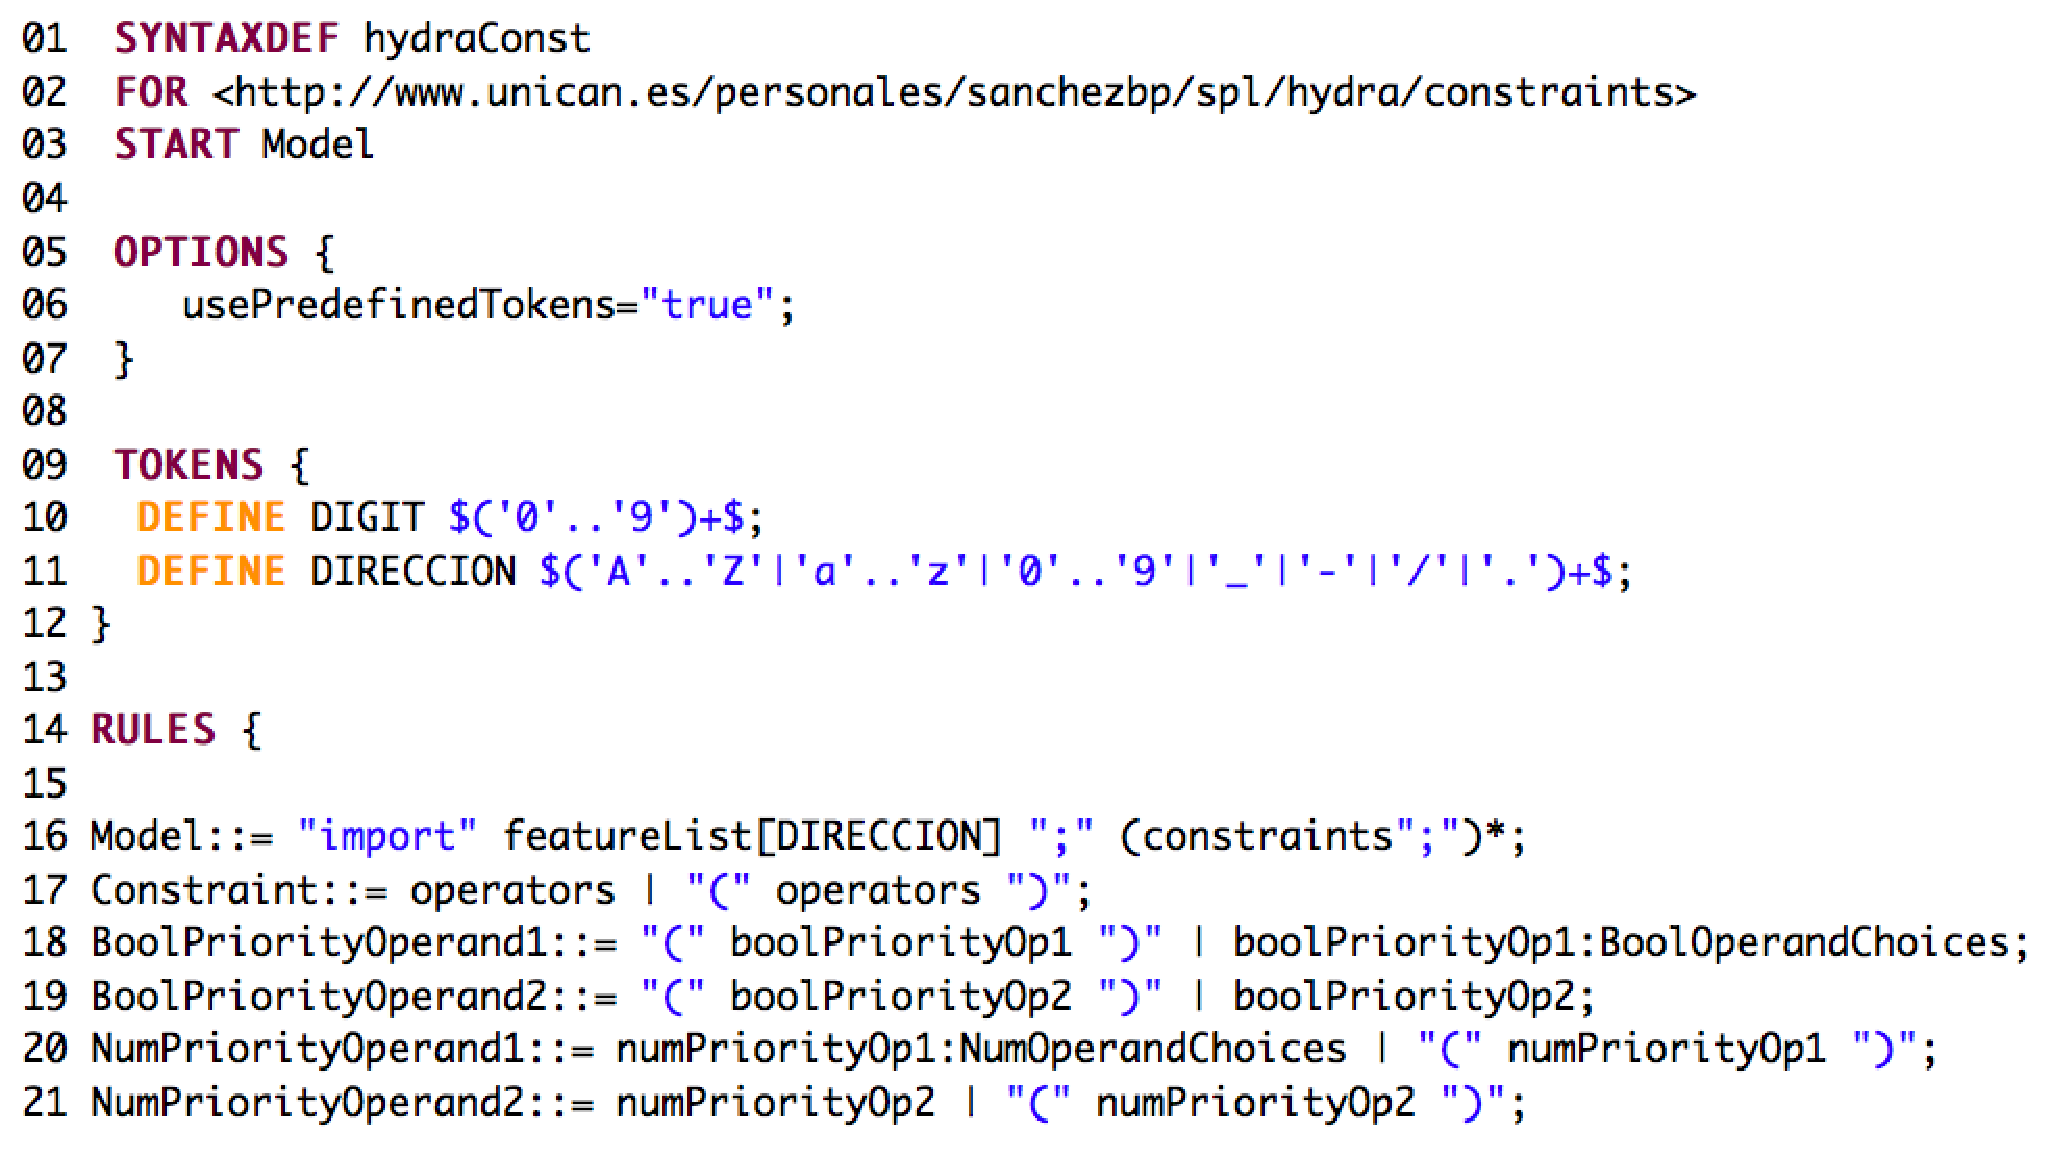
\includegraphics[scale=0.35]{gramatica/iniciogram.eps}
\caption{Implementaci�n del inicio de la gram�tica con EMFText. Con las figuras \ref{fig:opersUno} y \ref{fig:opersDos} se completa la gram�tica}
\label{fig:initGram}
\end{figure}

La primera l�nea muestra la cla�sula SYNTAXDEF, que sirve para indicar la extensi�n que queramos que tengan los ficheros correspondientes a nuestro lenguaje. En nuestro caso, hemos elegido la extensi�n \emph{hydraconst}. A continuaci�n, la directriz FOR sirve para vincular la gram�tica con el metamodelo mediante una direcci�n de Eclipse llamada \emph{URI}. La siguiente l�nea contiene la cl�usula START, que indica cu�l es la metaclase inicial del metamodelo, es decir, la primera a la que se le aplica una regla. Cualqueir gram�tica que se quiera construir en EMFText ha de empezar por estas tres directrices.

Las l�neas de [05-07] corresponden al bloque OPTIONS. Dentro de este bloque EMFText permite especificar diversas opciones para configurar nuestra gram�tica de diversos modos, que en su mayor�a afectan a la posterior generaci�n del c�digo que implementar�  el lenguaje. En nuestro caso solo hemos activado una opci�n, que permite usar los Tokens definidos por defecto en EMFText.

Entre las l�neas [09-12] se encuentra el bloque TOKENS. Este bloque sirve para definir los Tokens que usaremos en nuestra gram�tica. Un Token es un elemento terminal, es decir, uno cuyo derivaci�n no supone ninguna regla adicional para la gram�tica. En nuestro caso usaremos los Tokens para inicializar diversos atributos del metamodelo. El Token DIGIT ser� el que d� valor al atributo \emph{numValue} de la metaclase \emph{Number}, y el token DIRECCION ser� el utilizado para inicializar el atributo \emph{featureList} de la metaclase Model. Adem�s, usaremos el token TEXT para inicializar el atributo \emph{featureName} de las metaclases \emph{SimpleFeature} y \emph{MultipleFeature}. Este Token no hay que definirlo, ya que est� disponible por defecto al habilitar la opci�n previa \emph{usePredefinedTokens}.

Desde la l�nea 14 y hasta el final de la gram�tica estar� contenido el bloque RULES, que es en el que se definen las reglas de las que habl�bamos. La l�nea 16 contiene la regla de la metaclase inicial, Model. Esto significa que los textos que escribamos en nuestros lenguajes han de empezar siguiendo esta regla. En ella se define que la primera l�nea de cualquier c�digo escrito en nuestro lenguaje ha de empezar por la palabra reservada \emph{import}, y a continuaci�n se introduce la direcci�n que contiene el modelo de caracter�sticas sobre el que queremos aplicar las restricciones. Esta direcci�n se define por el Token DIRECCION y se guarda en el atributo \emph{featureList}. A partir de ah�, se indica que se han de escribir las restricciones.

La l�nea 17 contiene la regla correspondiente a la metaclase \emph{Constraint}. En ella simplemente se indica que a continuaci�n hay que escribir los diversos operadores, y se actualizan en el metamodelo las relaci�n llamada \emph{operators}. Las l�neas [18-21] sirven para implementar la prioridad en las operaciones, es decir, permitir la inclusi�n de par�ntesis en las operaciones.

\begin{figure}[t]
    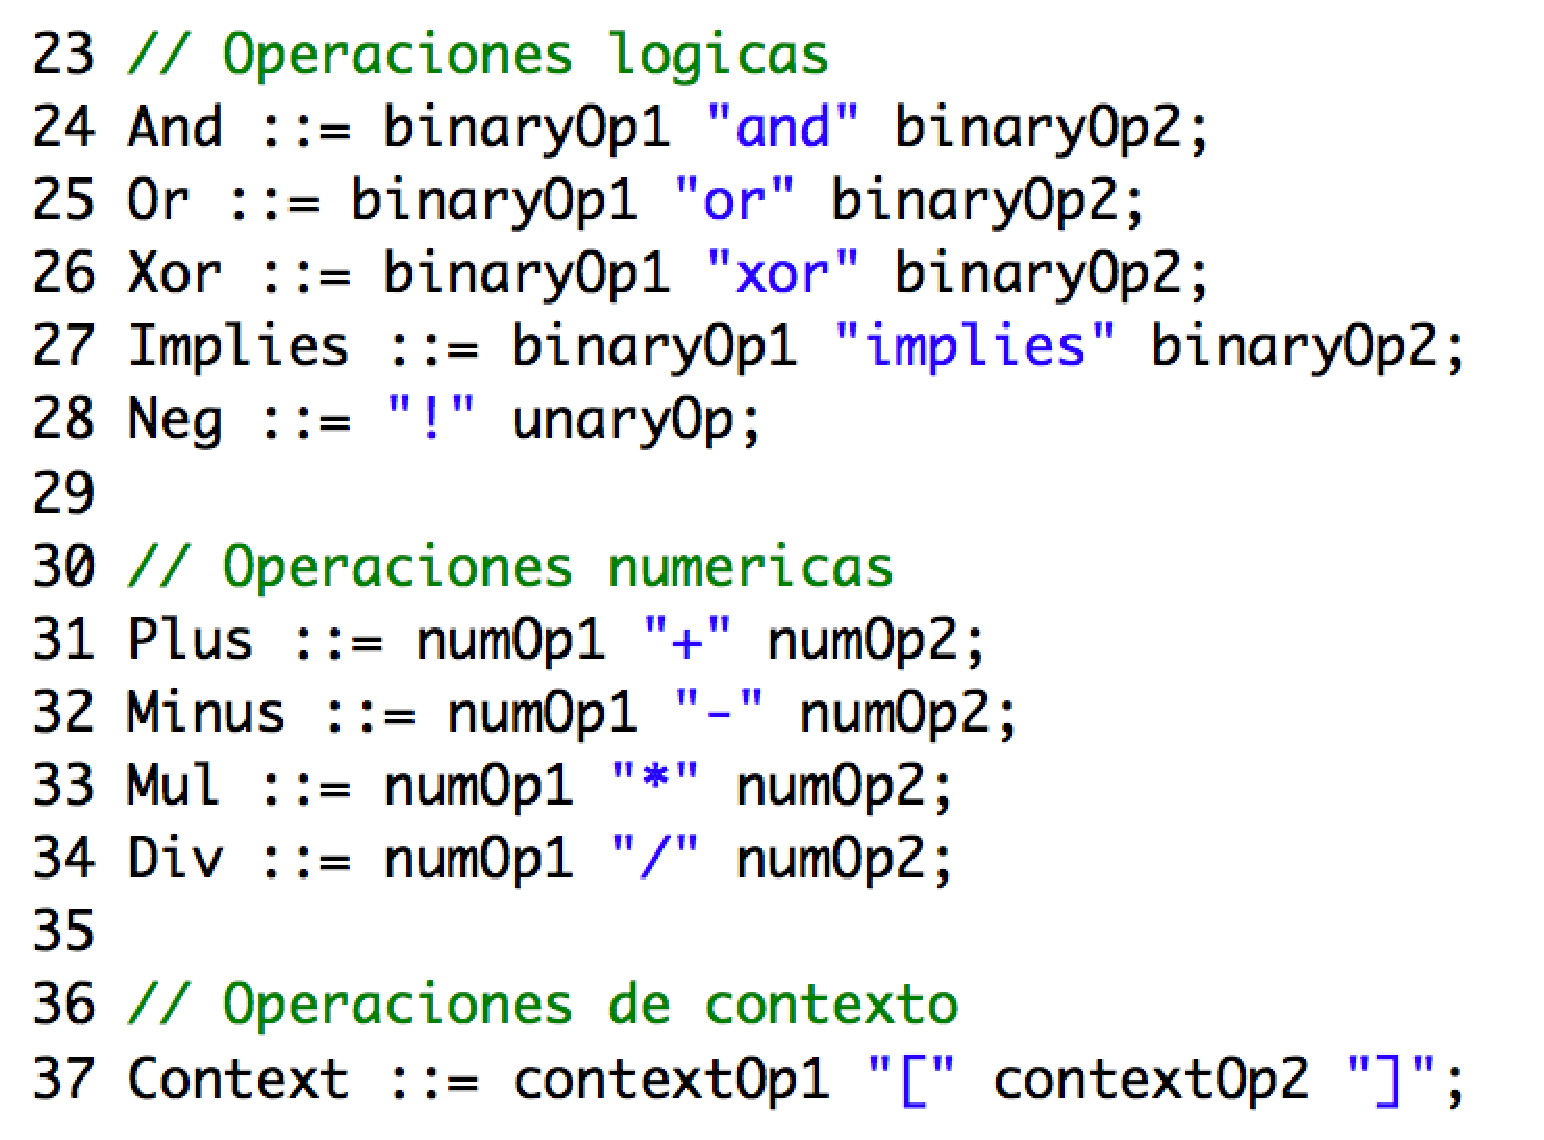
\includegraphics[scale=0.3]{gramatica/operaciones1.eps}
    \caption{Primera parte de la implementaci�n de las operaciones de nuestro editor com EMFText}
    \label{fig:opersUno}
\end{figure}

La Figura~\ref{fig:opersUno} contin�a directamente el trozo de gram�tica de la Figura~\ref{fig:initGram} y muestra las reglas correspondientes a una parte de las operaciones. 

Las l�neas [23-28] muestran las reglas para las operaciones l�gicas. Indican que la palabra reservada para la operaci�n de la metaclase \emph{And} es \emph{and}, y del mismo modo con las metaclases \emph{Or}, \emph{Xor} e \emph{Implies}. La palabra reservada para la operaci�n de la metaclase \emph{Not} es !. En estas reglas tambi�n se inicializan las relaciones \emph{binaryOp1}, \emph{binaryOp2} y \emph{unaryOp} al valor correspondiente. 

Las l�neas [30-34] muestran las reglas para las operaciones aritm�ticas. Indican que la palabra reservada para la operaci�n de la metaclase \emph{Plus} es $+$, para \emph{Minus} es $-$, para \emph{Mul} es $*$ y para \emph{Div} es $/$. En estas reglas tambi�n se inicializan las relaciones \emph{numOp1} y \emph{numOp2} al valor correspondiente. 

La l�nea 37 implementa la regla para la operaci�n correspondiente a la metaclase \emph{Context}. En ella se indica que un contexto se compone del operador \emph{contextOp2} rodeado entre corchetes precedido del operador \emph{contextOp1}. Ambos operadores son instanciados en sus debidas relaciones en el metamodelo.

\begin{figure}[t]
    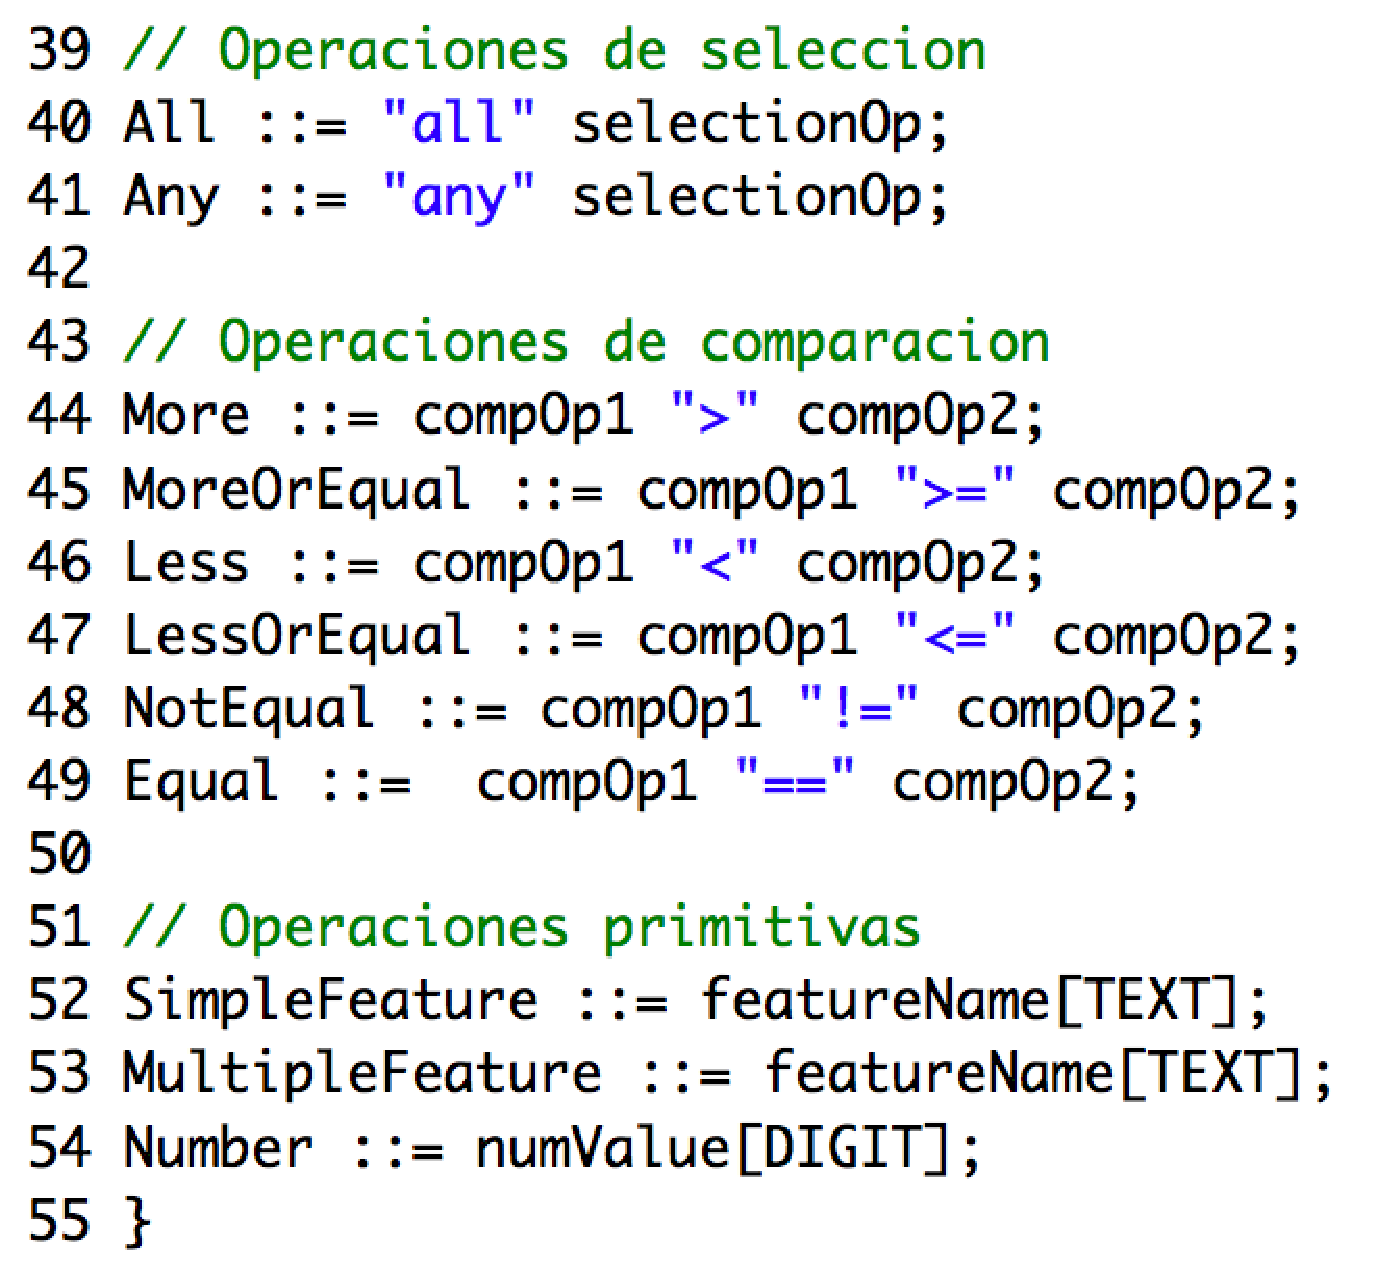
\includegraphics[scale=0.3]{gramatica/operaciones2.eps}
    \caption{Segunda parte de la implementaci�n de las operaciones de nuestro editor com EMFText}
    \label{fig:opersDos}
\end{figure}

La Figura~\ref{fig:opersDos} contin�a directamente el trozo de gram�tica de la Figura~\ref{fig:opersUno} y muestra la siguiente parte de la implementaci�n de las reglas de las operaciones.

Las l�neas [39-40] muestran las reglas para las operaciones correspondientes a las metaclases \emph{All} y \emph{Any}. En ambas se indica que la palabra reservada que las identifica es \emph{all} y \emph{any} respectivamente, y que a continuaci�n se ha de indicar el operador \emph{selectionOp}. Si miramos el metamodelo, veremos que este operador corresponde a una relaci�n con una operaci�n de contexto, con lo cual en este momento habr�a que introducir una restricci�n entre corchetes precedida de una caracter�stica que marque el contexto en que se eval�a. 

Las l�neas [43-49] muestran las reglas para las operaciones de comparaci�n. Indican que la palabra reservada para la operaci�n de la metaclase \emph{More} es $>$, para \emph{MoreOrEqual} es $>=$, para \emph{Less} es $<$, para \emph{LessOrEqual} es $<=$, para \emph{NotEqual} es $!=$ y para \emph{Equal} es $==$. En estas reglas tambi�n se inicializan las relaciones \emph{compOp1} y \emph{compOp2} al valor correspondiente. 

Para finalizar, las l�neas [51-54] muestran las operaciones primitivas. En el lenguaje, estas reglas corresponden a inicializar el atributo \emph{featureName} con el nombre de la caracter�stica que hayamos introducido, y del mismo modo, el atributo \emph{numValue} con el del n�mero que hayamos escrito.
%La parte m�s trivial e inmediata del dise�o de la gram�tica es la concerniente a la implementaci�n de las operaciones, pues las producciones necesarias simplemente requieren la inclusi�n de los operandos involucrados y los caracteres que deseemos que definan la operaci�n. La figura \ref{figopers} muestra la implementaci�n de estas operaciones.
%
%\begin{figure}[t]
%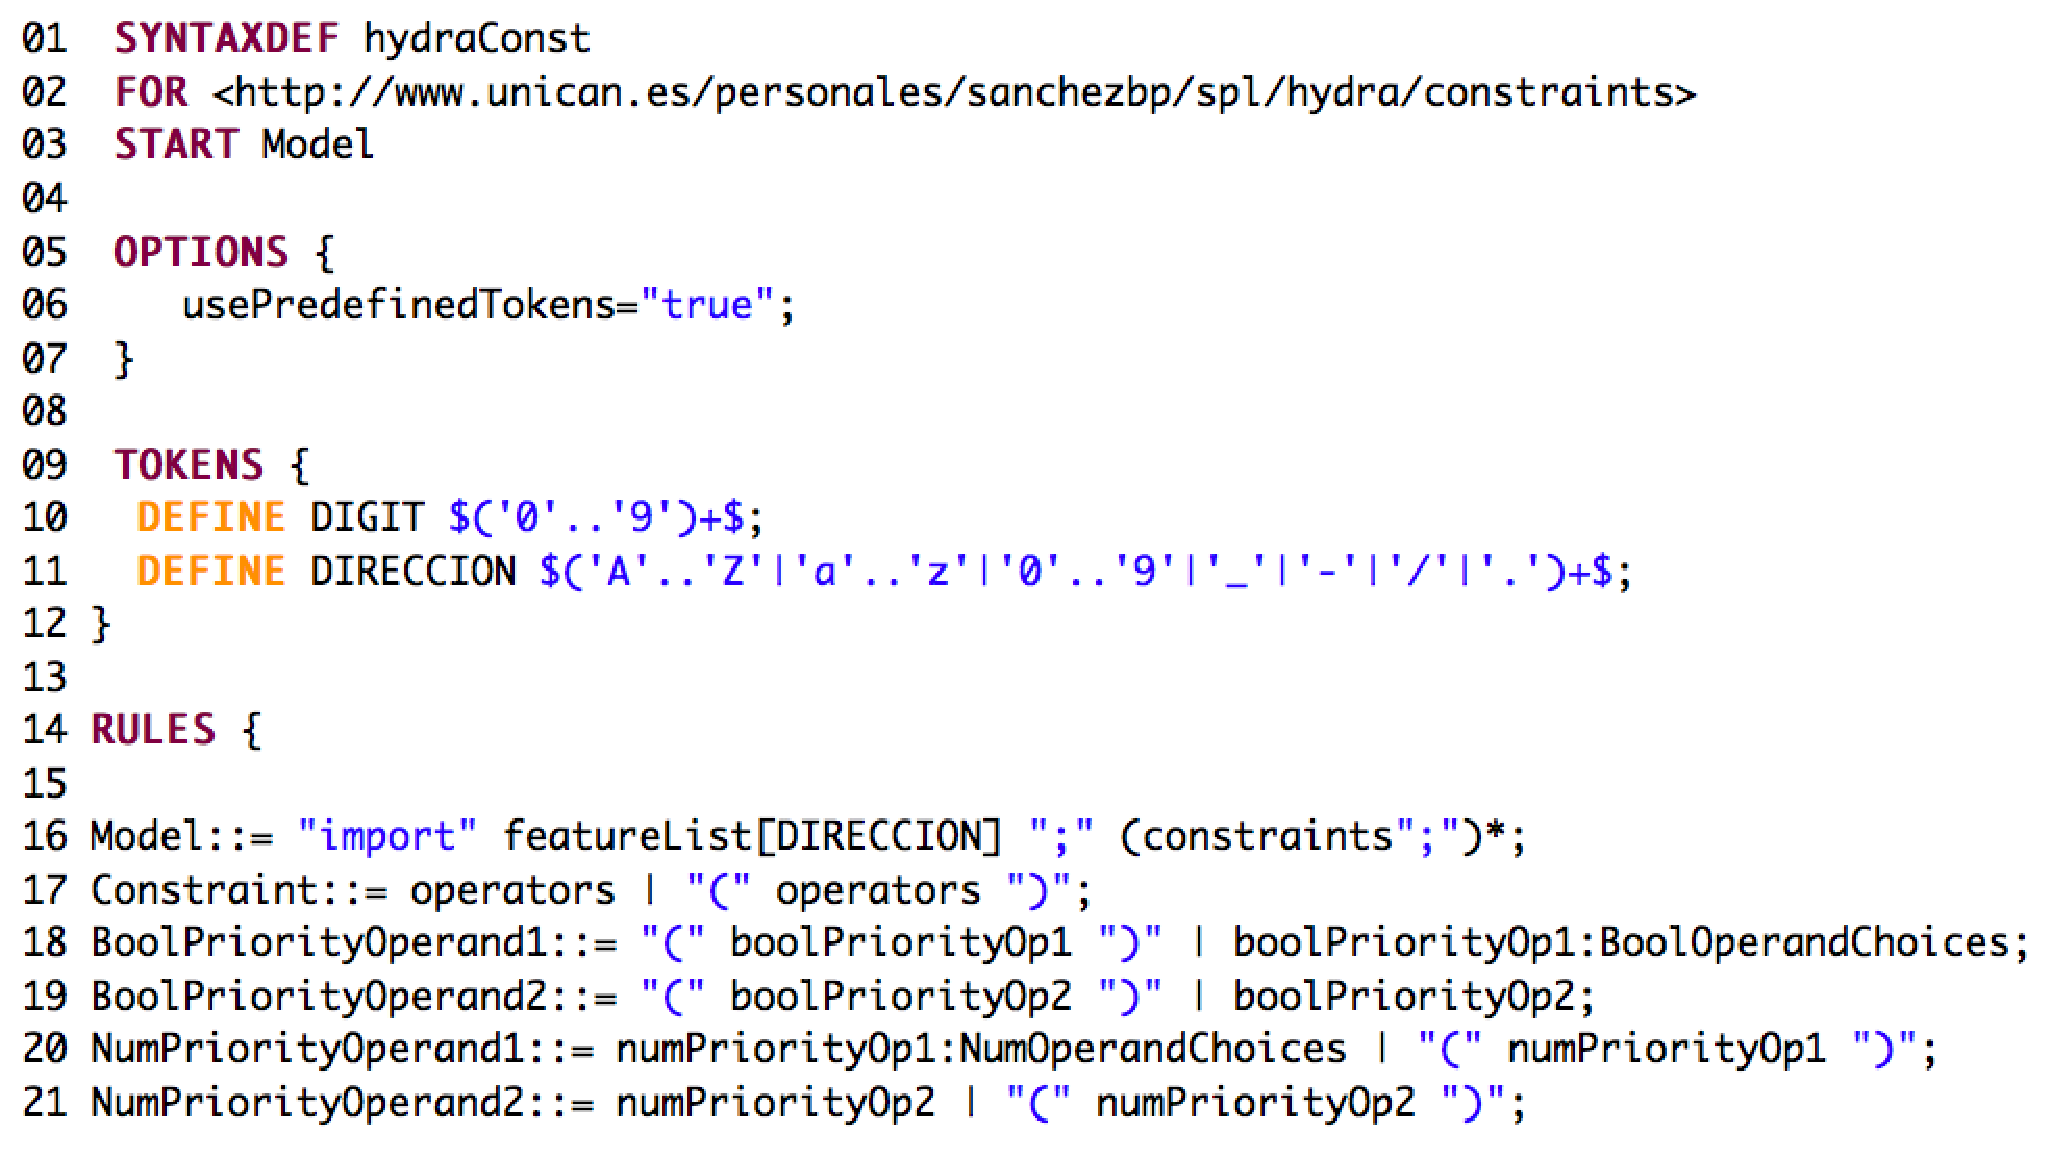
\includegraphics[scale=0.35]{gramatica/iniciogram.eps}
%\caption{Implementaci�n del inicio de la gram�tica con EMFText. Con la figura \ref{figopers} se completa la gram�tica}
%\label{figinitgram}
%\end{figure}
%
%\begin{figure}[t]
%    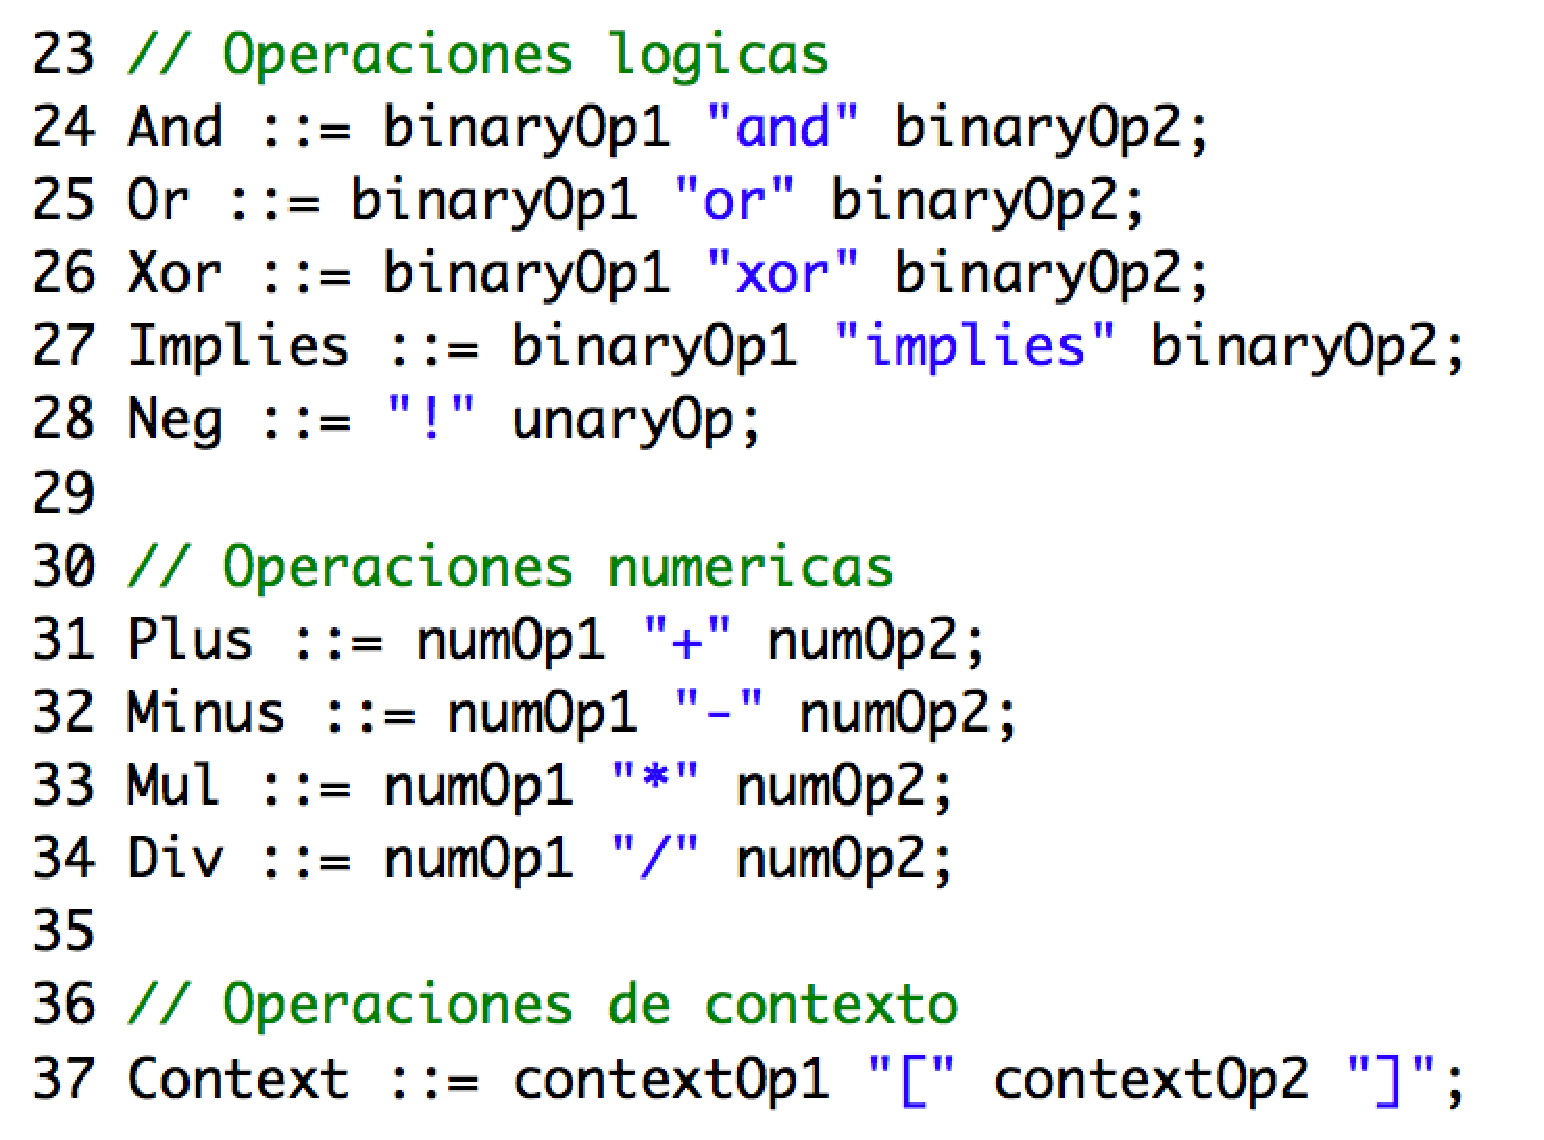
\includegraphics[scale=0.3]{gramatica/operaciones1.eps}
%    \caption{Implementaci�n de las operaciones de nuestro editor com EMFText}
%    \label{figopers}
%\end{figure}
%
%S� que cabe comentar con respecto a las operaciones las �ltimas l�neas, que muestran la asignaci�n de valor a las hojas de nuestros �rboles parseados. En esas l�neas estamos indicando que los atributos de las instancias de clase Number van a ser n�meros, y que los atributos de las instancias de las clases SimpleFeature y MultipleFeature van a ser palabras.
%
%La parte m�s complicada corresponde a la implementaci�n del inicio de la gram�tica y de las producciones que conducen a la misma. Pero antes de mostrar la figura con esta parte de la gram�tica conviene explicar el problema que llev� a realizar los cambios en el metamodelo mencionados en el cap�tulo anterior. Este problema surgi� a la hora de implementar las operaciones con prioridad, es decir, la inclusi�n de los par�ntesis.
%
%El inconveniente es que el tipo de gram�tica LL que implementa EMFText hac�a imposible tomar una decisi�n sobre hacia qu� elemento seguir parseando en caso de encontrarnos con un par�ntesis. La mejor soluci�n que se nos ocurri� para evitar este problema fue la adici�n de diversas clases y relaciones auxiliares en el metamodelo, cuya �nica funci�n es estructural y de apoyo a la gram�tica. Gracias a ellas y a una mejor definici�n de las producciones conseguimos evitar esos problemas de parsing y podemos llevar a cabo las operaciones de prioridad con par�ntesis.
%
%Las clases a�adidas para solventar esta situaci�n fueron las siguientes: BoolPriorityOperand1, BoolPriorityOperand2, NumPriorityOperand1, NumPriorityOperand2, BoolOperandChoices y NumOperandChoices. Las relaciones a�adidas fueron boolPriorityOp1, boolPriorityOp2, numPriorityOp1 y numPriorityOp2.
%
%Una situaci�n similar fue la que propici� que las operaciones Context, All y Any hayan sido dise�adas tal y como presenta el metamodelo, ya que que la particular sintaxis de estas (diferente a las dem�s que siguen el mismo esquema de op + char + op) tambi�n mostraba ciertos problemas de parsing. En este caso no fue necesario a�adir elementos auxiliares, sino simplemente recolocarlos para evitar estos problemas. Con esto ya se han hecho todos los cambios en el metamodelo, que alcanza en este punto su versi�n final tal como muestra la figura \ref{figmetameta}. Con respecto al metamodelo solamente quedan por comentar los m�todos que muestran algunas clases, que ser�n explicados en los pr�ximos cap�tulos ya que se usan en el proceso de validaci�n y sem�ntica.
%
%
%
%Una vez comentados estos detalles es momento de explicar el inicio de la gram�tica, que se muestra en la figura \ref{figinitgram}.
%
%En la primera l�nea y mediante la cla�sula SYNTAXDEF indicamos la extensi�n que queremos que tengan los ficheros escritos en nuestro lenguaje. En nuestro caso nos hemos decantado por la terminaci�n .hydraConst. En la segunda l�nea y mediante la cla�sula FOR se indica la URI del metamodelo. Una URI es un formato de direcci�n interno de Eclipse, que se usa para localizar otros ficheros en el workspace. En la tercera l�nea, delimitada por la cla�sula START, indicamos a la gram�tica que la clase inicial de nuestro metamodelo (y la que ser� la raiz en todos los �rboles parseados) es Model.
%
%El bloque OPTIONS permite activar algunas opciones de configuraci�n que incluye EMFText. En nuestro caso la �nica que tiene utilidad es usePredifinedTokens, que permite ahorrarnos la definici�n del token text. El bloque TOKENS sirve para definir los tokens de nuestra gram�tica. En nuestro caso usaremos 3: DIGIT para asignar al valor num�rico, TEXT para asignar a las caracter�sticas y DIRECCION para asignar la direcci�n f�sica del modelo de caracter�sticas.
%
%Por �ltimo, el bloque RULES permite crear las producciones. Como inicial, tal y como se especific� en los requisitos, exigimos un import y una direcci�n, que ser� almacenada en el atributo featureList de la clase Model. En la l�nea inicial tambi�n se indica, mediante una expresi�n regular, que el n�mero de restricciones a definir puede ser tan grande como se desee y que estas deben acabar con el car�cter '';'' .
%
%\begin{figure}[t]
%    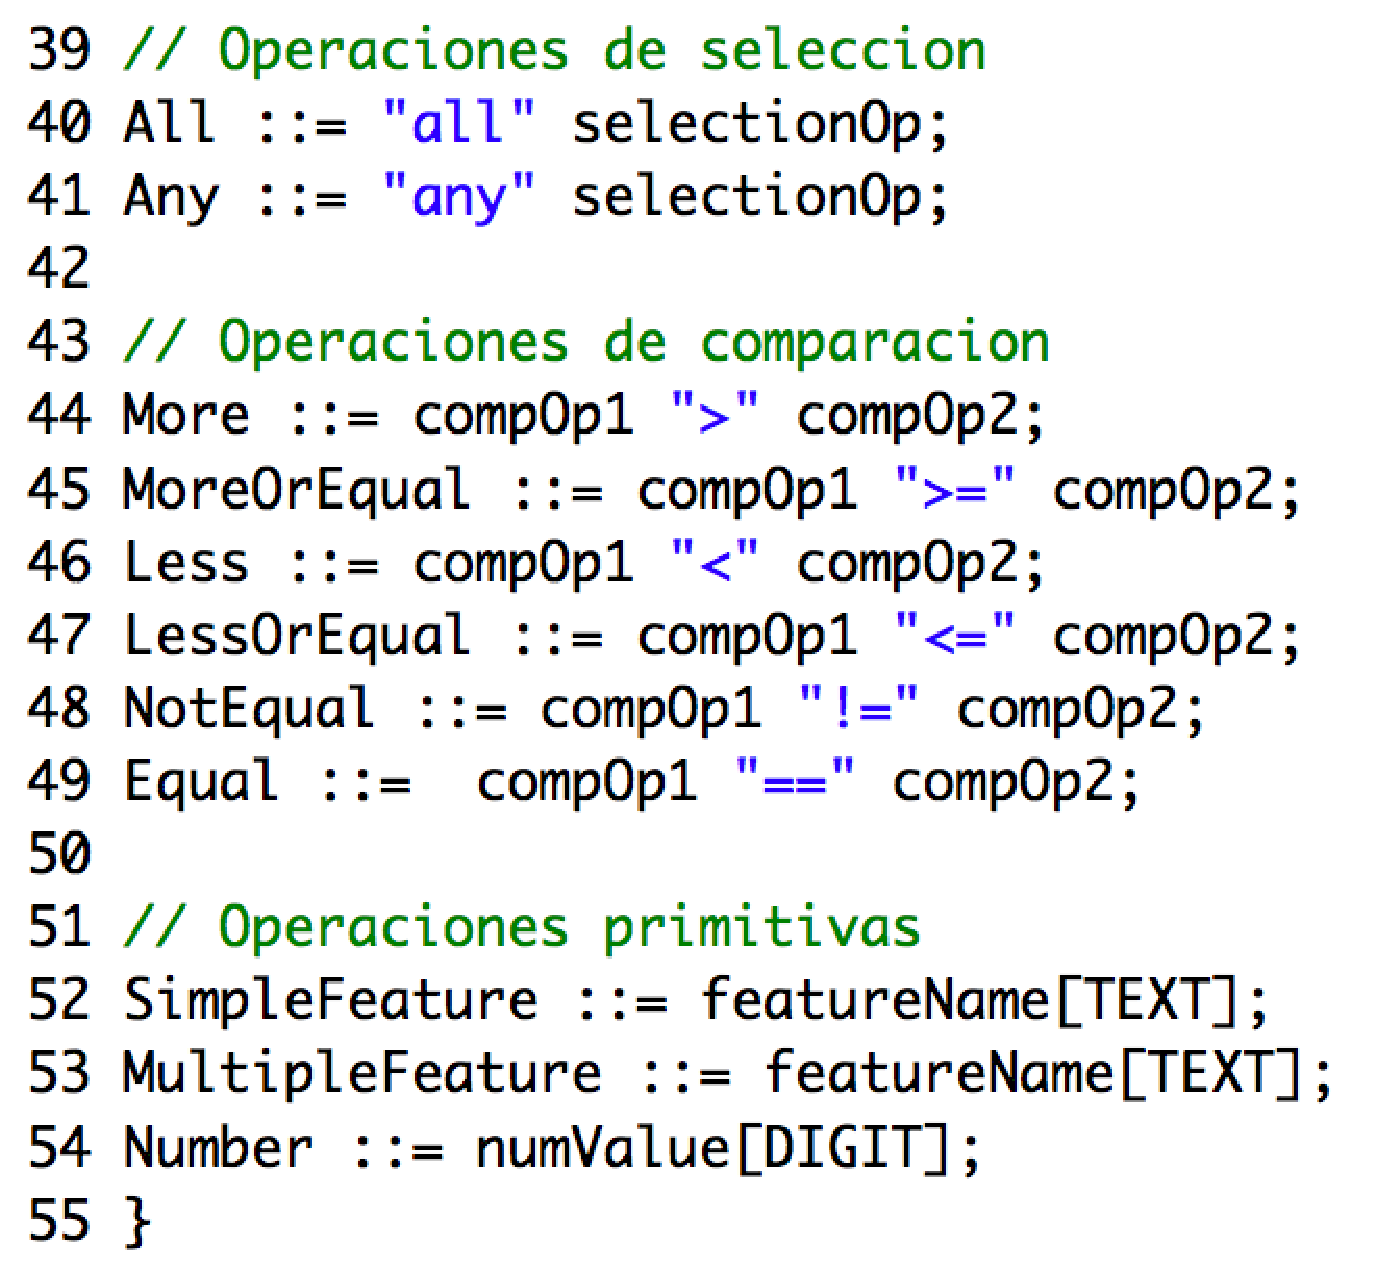
\includegraphics[scale=0.3]{gramatica/operaciones2.eps}
%    \caption{Implementaci�n de las operaciones de nuestro editor com EMFText}
%    \label{figopers}
%\end{figure}
%
%La l�nea de producci�n de Constraint diferencia entre operaciones con prioridad y sin ella. Sin el problema comentado de EMFText la gram�tica podr�a quedar as�, pero para solucionarlo nos vemos obligado a incluir las cuatro l�neas siguientes, cuya �nica funci�n es solventar esa situaci�n. El resto de la gram�tica continuar�a en la figura \ref{figopers} mostrada anteriormente, y ah� terminar�a.






\section{Pruebas}
\label{sec:gram:pruebas}
%%==================================================================%%
%% Author : Tejedo Gonz�lez, Daniel                                 %%
%%          S�nchez Barreiro, Pablo                                 %%
%% Version: 1.0, 25/11/2012                                         %%
%% Version: 1.0, 06/02/2013                                         %%
%%                                                                  %%
%% Memoria del Proyecto Fin de Carrera                              %%
%% Sintaxis abstracta,  pruebas                                     %%
%%==================================================================%%

Una vez creado nuestro metamodelo, deb�amos probar que dicho metamodelo era correcto. Es decir, que permit�a especificar todas las restricciones que dese�bamos crear, a la vez que, por construcci�n, imped�a la especificaci�n de restricciones que deb�an ser consideradas como sint�cticamente incorrectas.

Para ello realizamos una serie de pruebas consistentes en la creaci�n de varias instancias del metamodelo y observar el �rbol de sintaxis abstracta generado, comprobando si �ste se correspond�a con el esperado.

\begin{figure}[t]
    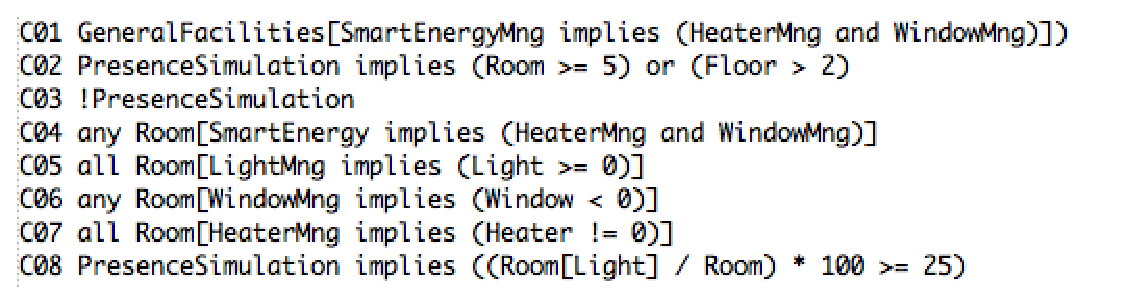
\includegraphics[scale=0.6]{metamodelo/instpruebas.eps}
    \caption{Conjunto de instrucciones que puso a prueba el funcionamiento del metamodelo}
    \label{figmetains}
\end{figure}

Las instrucciones que fueron puestas a prueba fueron las que se ven en la Figura~\ref{figmetains}. Este conjunto de instrucciones servir�n como pruebas tambi�n en momentos m�s avanzados del desarrollo. Dicho conjunto de pruebas fue dise�ado para recoger de la forma m�s exhaustiva posible todas las combinaciones de metaclases posibles.


% Cap�tulo 5: Creacion de la semantica
% %%==================================================================%%
%% Author : Tejedo Gonz�lez, Daniel                                 %%
%%          S�nchez Barreiro, Pablo                                 %%
%% Version: 1.0, 27/11/2012                                         %%                   %%                                                                  %%
%% Memoria del Proyecto Fin de Carrera                              %%
%% Gram�tica,  archivo raiz                                       %%
%%==================================================================%%

\chapterheader{Creaci�n de la gram�tica}{Creaci�n de la gram�tica}
\label{chap:gramatica}

Una vez ha sido definido el metamodelo, el siguiente paso es definir la sintaxis concreta textual de nuestro lenguaje, es decir, los medios que permitan expresarnos en �l de modo escrito. De no hacerlo, solo podr�amos usar este lenguaje creando instancias del metamodelo, lo cual l�gicamente no es ni c�modo ni conveniente. Este cap�tulo versa sobre la creaci�n de la gram�tica que permite definir esa sintaxis textual, as� como de las repercusiones que su dise�o tuvo en la sintaxis abstracta.

\chaptertoc

\section{Captura de requisitos}
\label{sec:gram:requisitos}
%%==================================================================%%
%% Author : Tejedo Gonz�lez, Daniel                                 %%
%%          S�nchez Barreiro, Pablo                                 %%
%% Version: 1.0, 25/11/2012                                         %%
%% Version: 2.0, 06/02/2013                                         %%
%%                                                                  %%
%% Memoria del Proyecto Fin de Carrera                              %%
%% Sintaxis abstracta, requisitos                                   %%
%%==================================================================%%

El primer paso para desarrollar nuestro lenguaje era conocer qu� aspecto deb�a tener nuestro lenguaje y qu� restricciones deb�a satisfacer. Es decir, en primer lugar debemos realizar un proceso que podemos denominar de captura de requisitos para poder comprender qu� es lo que tiene que hacer exactamente el lenguaje que se pretende crear.

Concretamente nuestro lenguaje hab�a sido pr�cticamente definido por el profesor Pablo S�nchez, del Departamento de Matem�ticas, Estad�stica y Computaci�n de la Universidad de Cantabria, mediante notaci�n BNF. Dicha gram�tica, se muestra en la Figura~\ref{fig:constraintBNF}. Las ideas subyacentes a dicho lenguaje son las que se describen a continuaci�n. 

\begin{figure}[!tb]
    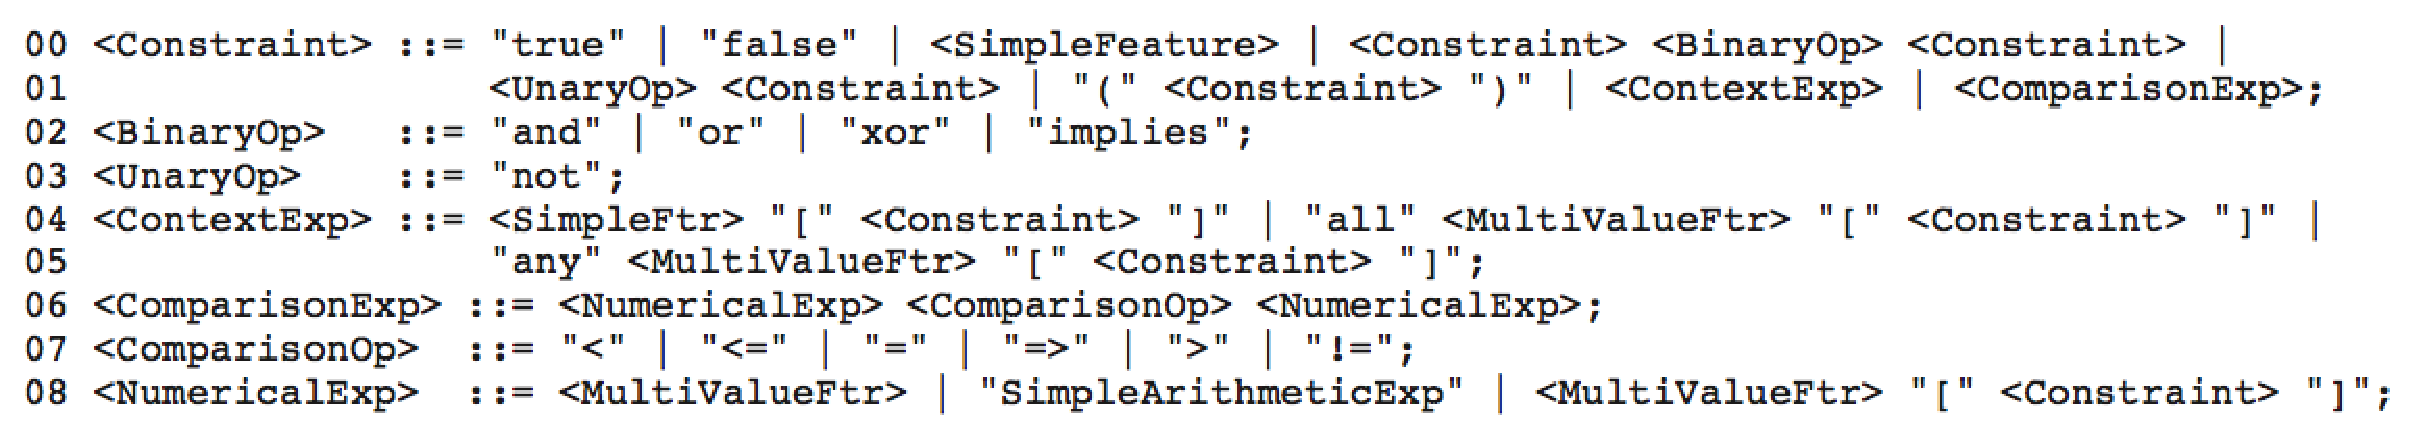
\includegraphics[scale=0.3]{metamodelo/constraintBNF.eps}
    \caption{Gram�tica en notaci�n BNF del lenguaje HCL}
    \label{fig:constraintBNF}
\end{figure}

En dicho lenguaje, una \emph{restricci�n} es una expresi�n l�gica que se puede evaluar a verdadero o falso. Una restricci�n puede ser simplemente un literal, es decir, $true$ o $false$, que se evaluar� a verdadero y falso respectivamente. Una restricci�n tambi�n puede ser una caracter�stica simple, es decir, una caracter�stica que puede aparecer en las configuraciones como m�ximo una vez. Una caracter�stica simple se eval�a a verdadero si ha sido seleccionada, y a falso en caso contrario.

Las caracter�sticas clonables son aquellas que pueden ser seleccionadas m�s de una vez en las configuraciones que construyamos sobre nuestro �rbol de caracter�sticas. Una caracter�stica clonable se eval�an como un n�mero entero positivo, incluido el cero. Ese n�mero representa el n�mero de clones que la caracter�stica posee dentro de una configuraci�n, o dicho de otro modo, el n�mero de veces que ha sido seleccionada. El hecho de que se eval�en como si fueran n�meros permite la inclusi�n de operaciones de comparaci�n entre distintas caracter�sticas clonables. Las operaciones de comparaci�n que se han de implementar son las siguientes: $<$,$<$=,$>$,$>=$,$=$,$!=$. Adem�s, tambi�n se puede utilizar el valor de las caracter�sticas clonables para implementar operaciones aritm�ticas b�sicas, tales como la suma, la resta, la multiplicaci�n y la divisi�n. Estas expresiones a su vez se pueden utilizar como subexpresiones, u operandos, dentro de las operaciones de comparaci�n. Las expresiones de comparaci�n se eval�an a verdadero o falso, y tambi�n pueden ser usadas como subexpresiones para crear expresiones l�gicas m�s complejas.

%%============================================================================%%
%% NOTA(Pablo) : Poner un ejemplo de este tipo de restricciones y explicarlas %%
%%============================================================================%%

Tal y como muestra la Figura~\ref{fig:constraintBNF}, una restricci�n tambi�n puede especificar un contexto concreto en el que poder evaluarla. Esto puede hacerse de varias maneras. Se puede especificar un contexto para una restricci�n poni�ndola entre corchetes y especificando el nombre de una caracter�stica al principio de la expresi�n. La caracter�stica usada como contexto puede ser tanto simple como m�ltiple. En el primer caso, la restricci�n s�lo ser� evaluada en el sub�rbol de la configuraci�n cuya ra�z sea la caracter�stica especificada.

%%============================================================================%%
%% NOTA(Pablo) : Poner un ejemplo y explicarlo                                %%
%%============================================================================%%

En el segundo caso entran en juego los operadores $all$ (para todo) y $any$ (existe). La operaci�n $all$ solo se evaluar� a verdadero si la restricci�n entre corchetes se cumple para todas las instancias de la caracter�stica clonable que act�a como contexto. En caso contrario, la operaci�n se evaluar� a falso. La operaci�n $any$ se evaluar� a verdadero si la restricci�n entre corchetes se cumple al menos una vez para todas las instancia de la caracter�stica clonable que act�a como contexto. Si la restricci�n no se cumple para ninguna de las selecciones, la operaci�n $any$ se evaluar� a falso.

%%============================================================================%%
%% NOTA(Pablo) : Poner un ejemplo y explicarlo                                %%
%%============================================================================%%

Merece la pena se�alar que una caracter�stica puede ser considera simple en un contexto determinado y clonable o m�ltiple en otro. Por ejemplo, la caracter�stica $LightMng$ es clonable en el contexto de $RoomFacilities$, pero simple en el contexto de $GeneralFacilities$. Debido a eso la caracter�stica $LightMng$ no puede ser utilizada sin especificar el contexto en el que est� ubicada, pues podr�a provocar un resultado no esperado o err�neo.

En la restricci�n $any Room[RoomFacilities[LightMng]]$ se pueden apreciar los dos diferentes usos para la operaci�n de contexto. Los corchetes externos indican a la operaci�n any que hay que aplicar la restricci�n a todas las habitaciones. Los corchetes internos indican que la caracter�stica $LightMng$ a la que se est� haciendo referencia es la hija de $RoomFacilities$ y no cualquier otra.

Adem�s nuestro lenguaje deb�a permitir vincular un modelo de caracter�sticas sobre el cual se definir�n un conjunto de restricciones externas. Este modelo se utilizar�, por ejemplo, para comprobar que los s�mbolos que aparecen como nombres de caracter�sticas en las restricciones se refieren a caracter�sticas que realmente existen en el �rbol de caracter�sticas. Por ejemplo, una restricci�n del tipo $AdvancedHeating => Heating$ carecer�a de sentido si algunas de las caracter�sticas $AdvancedHeating$ o $Heating$ no apareciesen en el �rbol de caracter�sticas sobre el cual estamos definiendo restricciones.

%%======================================================================================%%
%% NOTA(Pablo): Esto posiblemente sobre al introducir la traducci�n de la Secci�n III.
%%              Si es as�, eliminarla.
%%              Si los conceptos de restricci�n con contexto y operaci�n cuantificada
%%              no apareciesen, meter esta clasificaci�n pero resumida
%%======================================================================================%%
%%
%% De entre todos esos requisitos b�sicos, es necesario entrar en detalle en el n�mero 3
%% y enumerar la lista de operaciones que pueden ser definidas por nuestro lenguaje. Se
%% pueden clasificar en los siguientes tipos: \\
%%
%% - L�gicas: Son operaciones cuyos operandos han de ser caracter�sticas sin
%%   cardinalidad (tambi�n llamadas caracter�sticas simples), y que se evaluan a
%%   verdadero o falso. Entre las operaciones l�gicas encontramos las cl�sicas not,
%%   and, or, xor e implica.
%%
%% - Num�ricas: Sus operandos han de ser caracter�sticas con cardinalidad (tambi�n
%%   llamadas caracter�sticas m�ltiples) o simplemente n�meros. Su resultado se evalua
%%   con un valor num�rico. Las operaciones num�ricas a implementar son la suma, resta,
%%   multiplicaci�n y divisi�n.
%%
%% - Comparativas: Sus operandos han de ser caracter�sticas m�ltiples o simplemente n�meros,
%%   pero su resultado se evalua con un valor booleano. Las operaciones de comparaci�n a
%%   implementar son igual que, mayor que, menor que, distinto que, mayor o igual que y menor
%%   o igual que.
%%
%% - Operaci�n de contexto: Operaci�n que permite hacer referencia a una caracter�stica
%%   hija de otra caracter�stica. Esta operaci�n tiene sentido para seleccionar
%%   caracter�sticas cuyo nombre pueda estar repetido pero que tengan contextos diferentes.
%%   Por ejemplo, en el modelo de caracter�sticas SmartHome de la figura \ref{figsmarthome}
%%   podemos observar que la caracter�stica HeaterMng est� presente en muchos contextos
%%   diferentes. Esta operaci�n es necesaria para poder saber con seguridad a cual de esos
%%   contextos estamos aplicando la restricci�n.
%%
%% - Operaci�n de selecci�n: Operaci�n que corresponde a los operadores l�gicos cl�sicos
%%   "para todo" o "existe", y que tiene la misma funcionalidad. Evalua si una restricci�n
%%   se cumple para todos los casos en que puede existir  o si se cumple en alguno de los
%%   casos. Por ejemplo, en el modelo de la figura \ref{figsmarthome} se podr�a evaluar una
%%   restricci�n para cada una de las habitaciones que hayan sido definidas, y saber si se
%%  cumple en todas, en alguna o en ninguna.
%%
%%======================================================================================%%

Utilizando esta informaci�n como base, procedimos a crear el correspondiente metamodelo en Ecore para nuestro lenguaje.




\section{Dise�o de la gramatica}
\label{sec:gram:design}
%%==================================================================%%
%% Author : Tejedo Gonz�lez, Daniel                                 %%
%%          S�nchez Barreiro, Pablo                                 %%
%% Version: 1.0, 27/11/2012                                         %%                   
%% Version: 2.0, 09/02/2013                                         %%                   
%%                                                                  %%
%% Memoria del Proyecto Fin de Carrera                              %%
%% Gram�tica, Dise�o                                                %%
%%==================================================================%%

Una vez han sido definidas las caracter�sticas que queremos que nuestra sintaxis textual posea, el siguiente paso es dise�ar una gram�tica que se ajuste a ellas. EMFText es la herramienta que utilizaremos para implementar esta gram�tica. 

El dise�o de la gram�tica pasa por asignar una serie de reglas a las metaclases, de modo que EMFText sea capaz de reconocer esas reglas en las expresiones de nuestro lenguaje y asociarlas a la metaclase correspondiente. En cuanto la reconozca, a�adir� una instancia de la misma, con los atributos correspondientes debidamente inicializados, a la instancia global del metamodelo.

Adem�s de las reglas, en EMFText hay que definir otra serie de cla�sulas que permiten configurar ciertos aspectos de la gram�tica. Para explicar tanto estas directrices como las reglas de las metaclases nos apoyaremos en la gram�tica dise�ada, y explicaremos l�nea a l�nea el significado de las instrucciones que la componen. La Figura~\ref{fig:initGram} muestra las primeras 23 l�neas de la gram�tica para nuestro lenguaje. 
%%=================================================================%%
%% NOTA(Pablo): Refresca aqu� un poco el proceso de desarrollo de  %%
%%              gram�ticas con EMFText, en uno o dos parr�fos a    %%
%%              muy alto nivel                                     %%   
%%=================================================================%%

%%=================================================================%%
%% NOTA(Pablo): Tal como est� escrito, es dif�cil seguir el hilo   %%
%%              argumental, vuelvo a escribirlo de forma top-down, %%
%%              describiendo, sin enrollarte mucho, lo que aparece %%
%%              en las figuras. Empieza por la segunda, por la     %%
%%              l�nea 1, y sigue para abajo                        %%
%%              Piensa en a�adirle n�meros de l�neas a las figuras %%
%%              para hacer m�s f�cil su descripci�n.               %%
%%              Haz especial hincapi� en como se relacionan la     %% 
%%              gram�tica con el metamodelo. 
%%              Evista el t�rmino producci�n, que es muy 
%%              espec�fico de procesdores de lenguajes, y no todos
%%              los miembros del tribunal lo van a entender
%%              Planteate usar el entorno listing para mostrar 
%%              c�digo
%%=================================================================%%

%%=================================================================%%
%% NOTA(Pablo): Estas figuras se ven fatal, no las metas como      %%
%%              capturas de pantalla o p�salas a EPS mejor         %%
%%=================================================================%%

\begin{figure}[t]
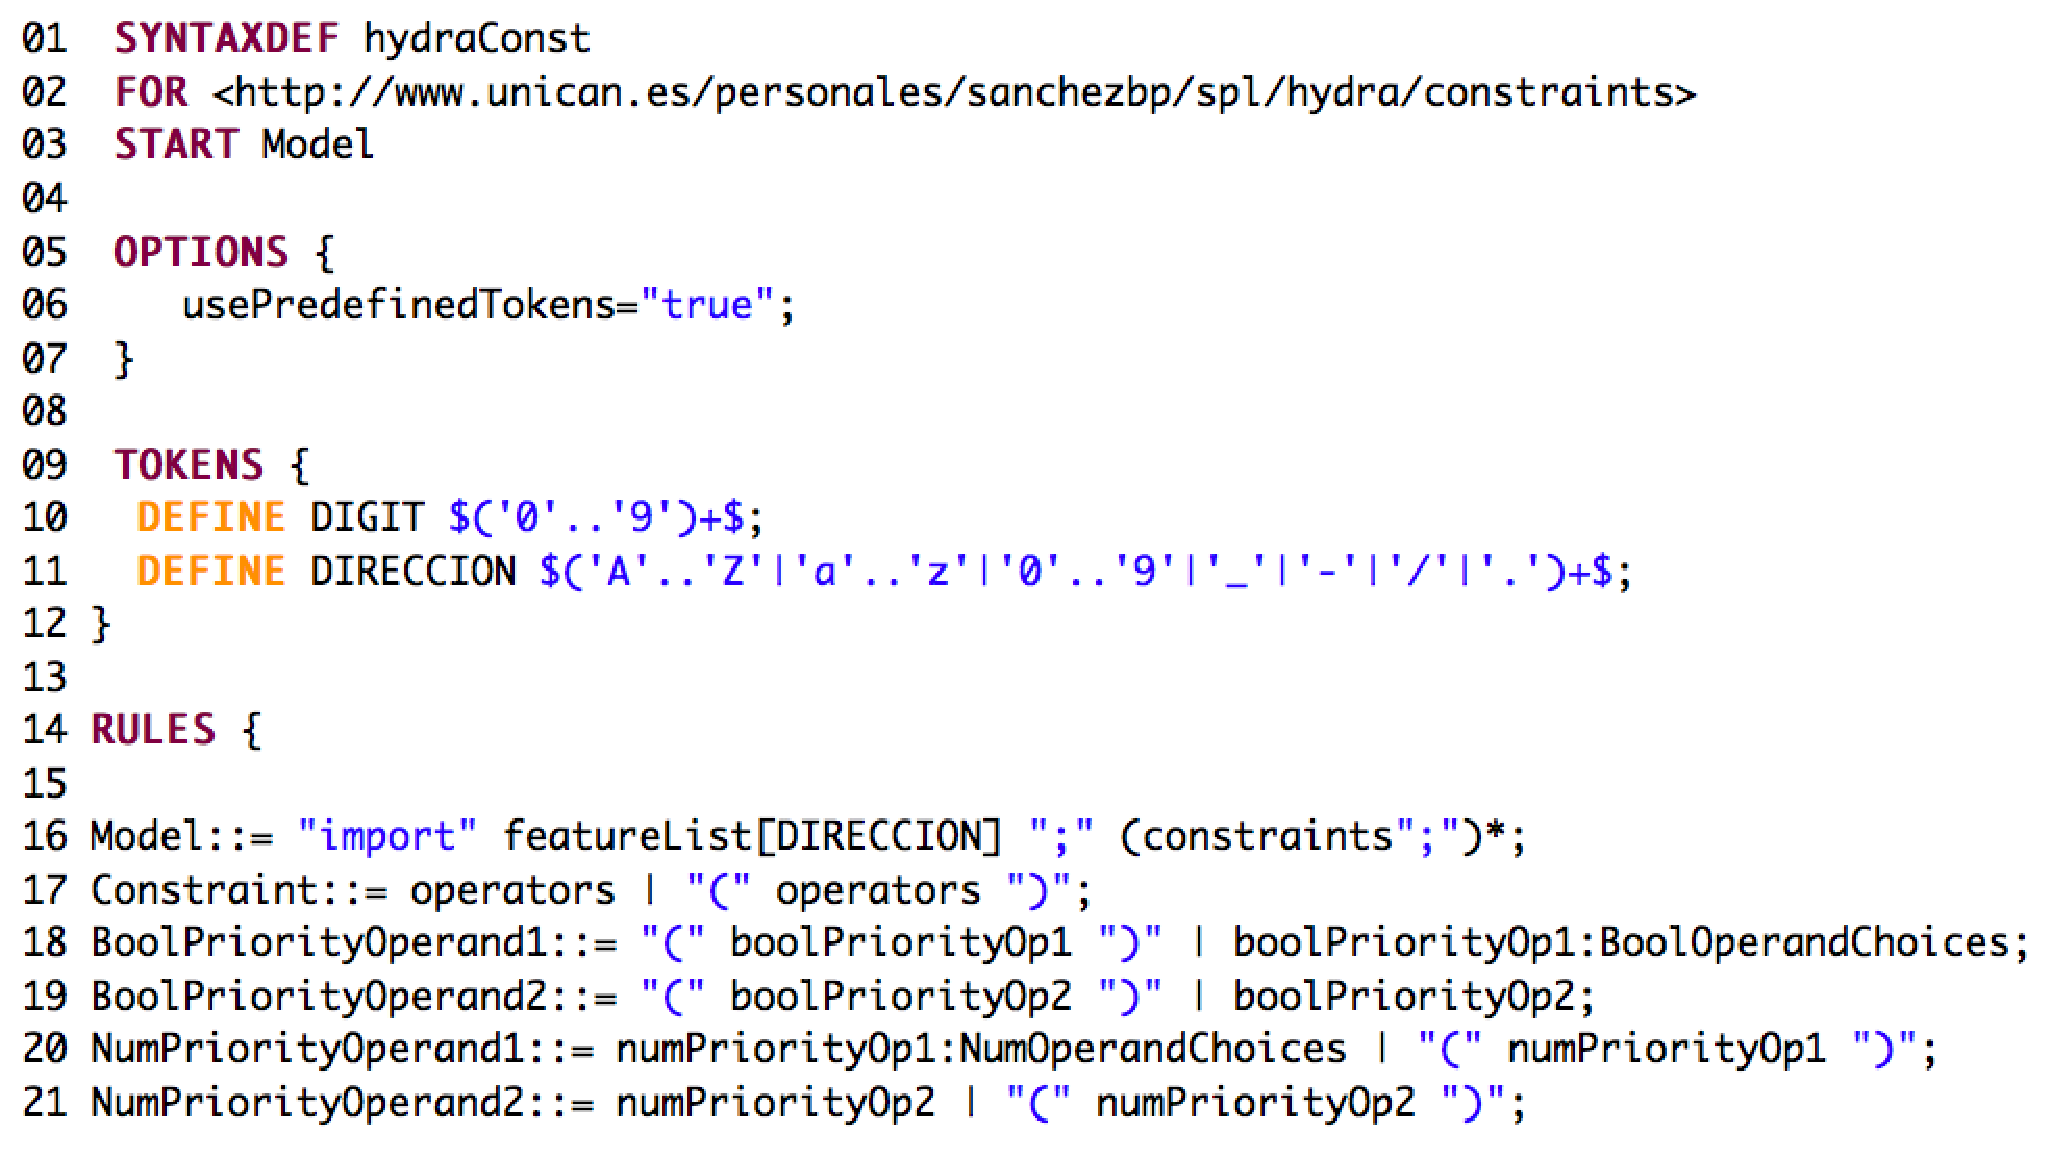
\includegraphics[scale=0.35]{gramatica/iniciogram.eps}
\caption{Implementaci�n del inicio de la gram�tica con EMFText. Con las figuras \ref{fig:opersUno} y \ref{fig:opersDos} se completa la gram�tica}
\label{fig:initGram}
\end{figure}

La primera l�nea muestra la cla�sula SYNTAXDEF, que sirve para indicar la extensi�n que queramos que tengan los ficheros correspondientes a nuestro lenguaje. En nuestro caso, hemos elegido la extensi�n \emph{hydraconst}. A continuaci�n, la directriz FOR sirve para vincular la gram�tica con el metamodelo mediante una direcci�n de Eclipse llamada \emph{URI}. La siguiente l�nea contiene la cl�usula START, que indica cu�l es la metaclase inicial del metamodelo, es decir, la primera a la que se le aplica una regla. Cualqueir gram�tica que se quiera construir en EMFText ha de empezar por estas tres directrices.

Las l�neas de [05-07] corresponden al bloque OPTIONS. Dentro de este bloque EMFText permite especificar diversas opciones para configurar nuestra gram�tica de diversos modos, que en su mayor�a afectan a la posterior generaci�n del c�digo que implementar�  el lenguaje. En nuestro caso solo hemos activado una opci�n, que permite usar los Tokens definidos por defecto en EMFText.

Entre las l�neas [09-12] se encuentra el bloque TOKENS. Este bloque sirve para definir los Tokens que usaremos en nuestra gram�tica. Un Token es un elemento terminal, es decir, uno cuyo derivaci�n no supone ninguna regla adicional para la gram�tica. En nuestro caso usaremos los Tokens para inicializar diversos atributos del metamodelo. El Token DIGIT ser� el que d� valor al atributo \emph{numValue} de la metaclase \emph{Number}, y el token DIRECCION ser� el utilizado para inicializar el atributo \emph{featureList} de la metaclase Model. Adem�s, usaremos el token TEXT para inicializar el atributo \emph{featureName} de las metaclases \emph{SimpleFeature} y \emph{MultipleFeature}. Este Token no hay que definirlo, ya que est� disponible por defecto al habilitar la opci�n previa \emph{usePredefinedTokens}.

Desde la l�nea 14 y hasta el final de la gram�tica estar� contenido el bloque RULES, que es en el que se definen las reglas de las que habl�bamos. La l�nea 16 contiene la regla de la metaclase inicial, Model. Esto significa que los textos que escribamos en nuestros lenguajes han de empezar siguiendo esta regla. En ella se define que la primera l�nea de cualquier c�digo escrito en nuestro lenguaje ha de empezar por la palabra reservada \emph{import}, y a continuaci�n se introduce la direcci�n que contiene el modelo de caracter�sticas sobre el que queremos aplicar las restricciones. Esta direcci�n se define por el Token DIRECCION y se guarda en el atributo \emph{featureList}. A partir de ah�, se indica que se han de escribir las restricciones.

La l�nea 17 contiene la regla correspondiente a la metaclase \emph{Constraint}. En ella simplemente se indica que a continuaci�n hay que escribir los diversos operadores, y se actualizan en el metamodelo las relaci�n llamada \emph{operators}. Las l�neas [18-21] sirven para implementar la prioridad en las operaciones, es decir, permitir la inclusi�n de par�ntesis en las operaciones.

\begin{figure}[t]
    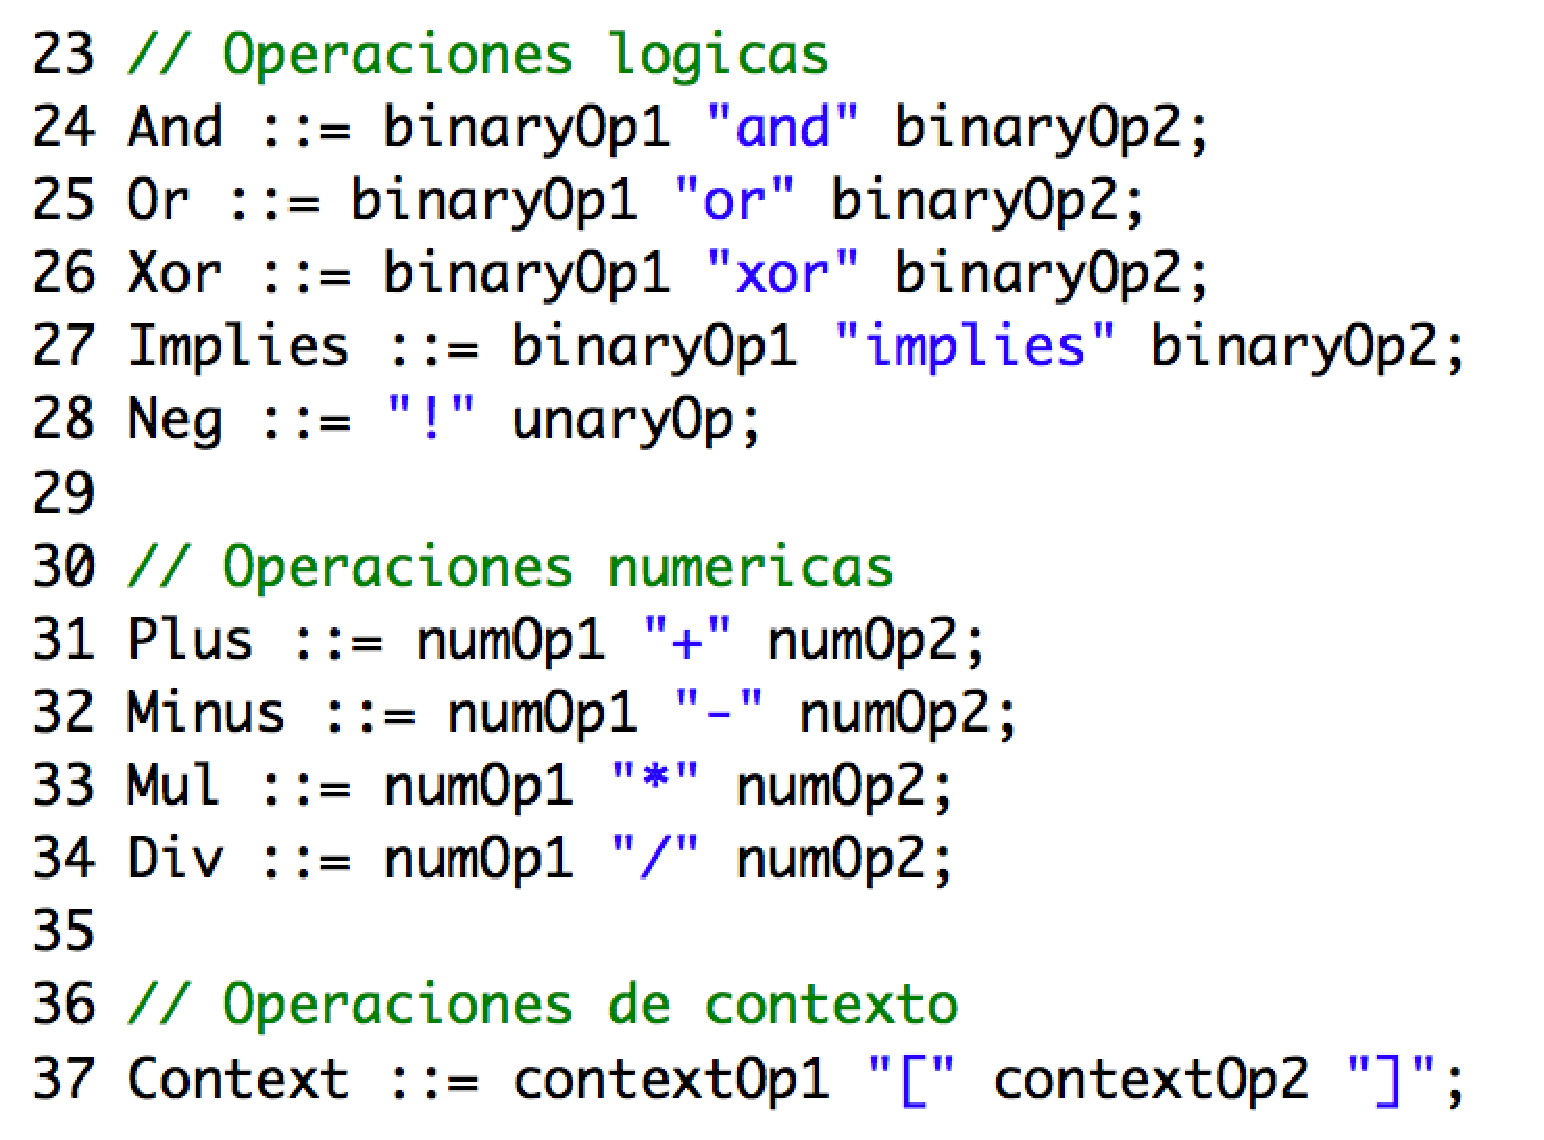
\includegraphics[scale=0.3]{gramatica/operaciones1.eps}
    \caption{Primera parte de la implementaci�n de las operaciones de nuestro editor com EMFText}
    \label{fig:opersUno}
\end{figure}

La Figura~\ref{fig:opersUno} contin�a directamente el trozo de gram�tica de la Figura~\ref{fig:initGram} y muestra las reglas correspondientes a una parte de las operaciones. 

Las l�neas [23-28] muestran las reglas para las operaciones l�gicas. Indican que la palabra reservada para la operaci�n de la metaclase \emph{And} es \emph{and}, y del mismo modo con las metaclases \emph{Or}, \emph{Xor} e \emph{Implies}. La palabra reservada para la operaci�n de la metaclase \emph{Not} es !. En estas reglas tambi�n se inicializan las relaciones \emph{binaryOp1}, \emph{binaryOp2} y \emph{unaryOp} al valor correspondiente. 

Las l�neas [30-34] muestran las reglas para las operaciones aritm�ticas. Indican que la palabra reservada para la operaci�n de la metaclase \emph{Plus} es $+$, para \emph{Minus} es $-$, para \emph{Mul} es $*$ y para \emph{Div} es $/$. En estas reglas tambi�n se inicializan las relaciones \emph{numOp1} y \emph{numOp2} al valor correspondiente. 

La l�nea 37 implementa la regla para la operaci�n correspondiente a la metaclase \emph{Context}. En ella se indica que un contexto se compone del operador \emph{contextOp2} rodeado entre corchetes precedido del operador \emph{contextOp1}. Ambos operadores son instanciados en sus debidas relaciones en el metamodelo.

\begin{figure}[t]
    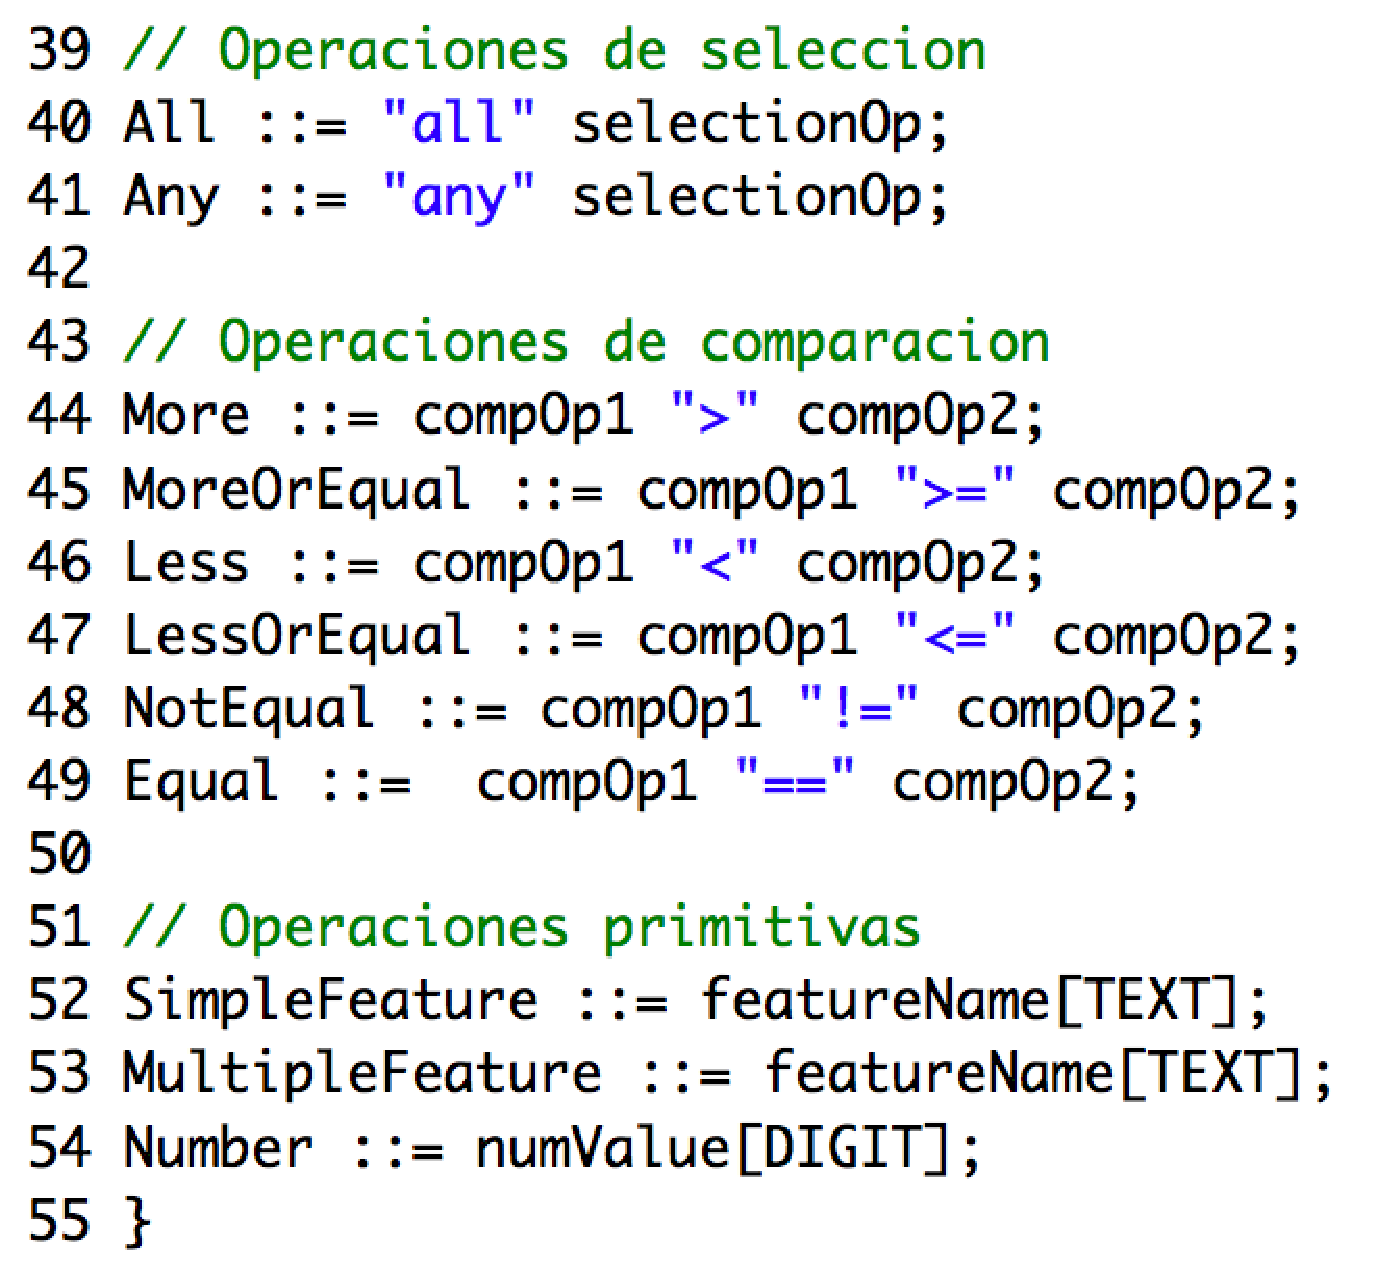
\includegraphics[scale=0.3]{gramatica/operaciones2.eps}
    \caption{Segunda parte de la implementaci�n de las operaciones de nuestro editor com EMFText}
    \label{fig:opersDos}
\end{figure}

La Figura~\ref{fig:opersDos} contin�a directamente el trozo de gram�tica de la Figura~\ref{fig:opersUno} y muestra la siguiente parte de la implementaci�n de las reglas de las operaciones.

Las l�neas [39-40] muestran las reglas para las operaciones correspondientes a las metaclases \emph{All} y \emph{Any}. En ambas se indica que la palabra reservada que las identifica es \emph{all} y \emph{any} respectivamente, y que a continuaci�n se ha de indicar el operador \emph{selectionOp}. Si miramos el metamodelo, veremos que este operador corresponde a una relaci�n con una operaci�n de contexto, con lo cual en este momento habr�a que introducir una restricci�n entre corchetes precedida de una caracter�stica que marque el contexto en que se eval�a. 

Las l�neas [43-49] muestran las reglas para las operaciones de comparaci�n. Indican que la palabra reservada para la operaci�n de la metaclase \emph{More} es $>$, para \emph{MoreOrEqual} es $>=$, para \emph{Less} es $<$, para \emph{LessOrEqual} es $<=$, para \emph{NotEqual} es $!=$ y para \emph{Equal} es $==$. En estas reglas tambi�n se inicializan las relaciones \emph{compOp1} y \emph{compOp2} al valor correspondiente. 

Para finalizar, las l�neas [51-54] muestran las operaciones primitivas. En el lenguaje, estas reglas corresponden a inicializar el atributo \emph{featureName} con el nombre de la caracter�stica que hayamos introducido, y del mismo modo, el atributo \emph{numValue} con el del n�mero que hayamos escrito.
%La parte m�s trivial e inmediata del dise�o de la gram�tica es la concerniente a la implementaci�n de las operaciones, pues las producciones necesarias simplemente requieren la inclusi�n de los operandos involucrados y los caracteres que deseemos que definan la operaci�n. La figura \ref{figopers} muestra la implementaci�n de estas operaciones.
%
%\begin{figure}[t]
%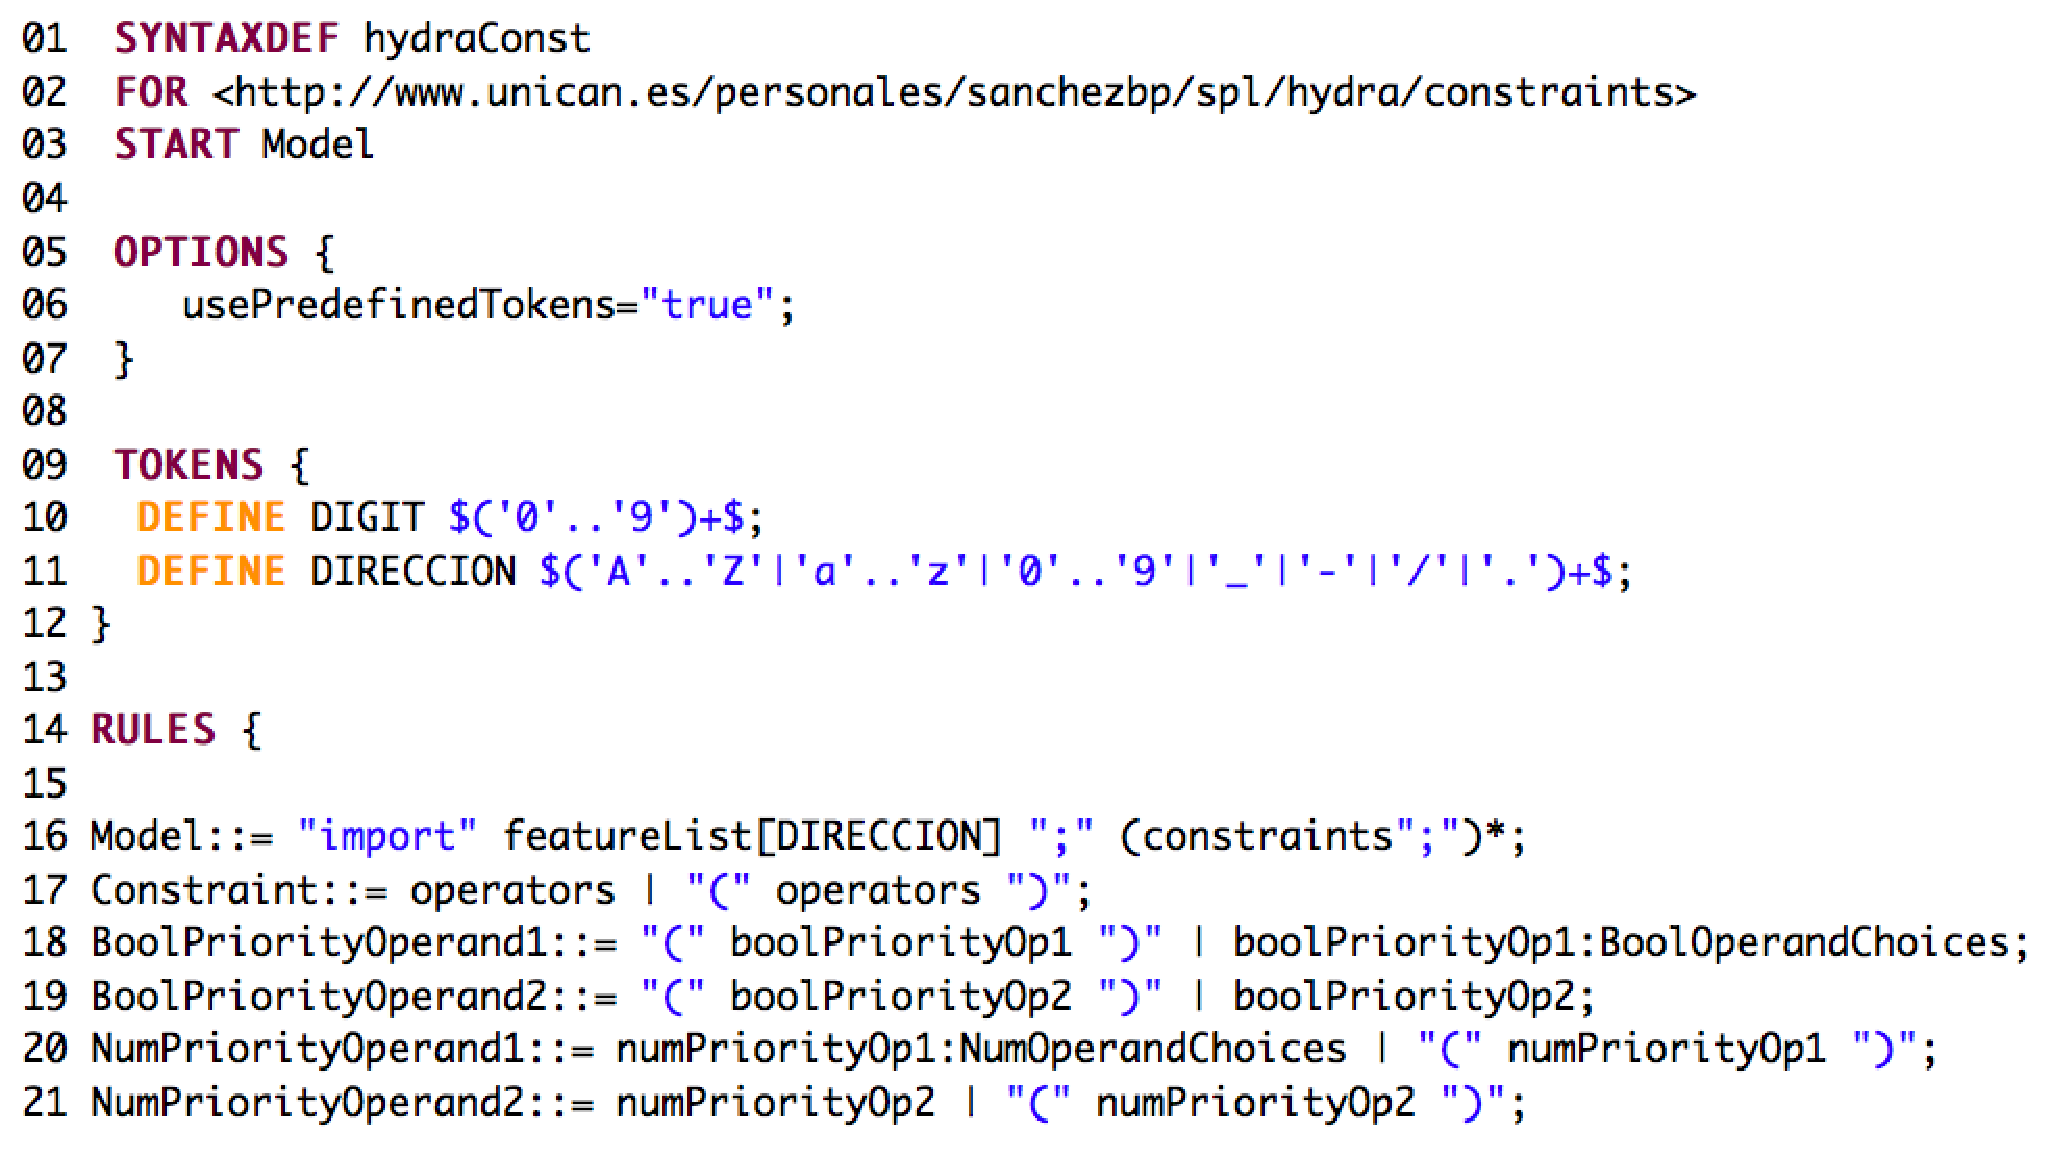
\includegraphics[scale=0.35]{gramatica/iniciogram.eps}
%\caption{Implementaci�n del inicio de la gram�tica con EMFText. Con la figura \ref{figopers} se completa la gram�tica}
%\label{figinitgram}
%\end{figure}
%
%\begin{figure}[t]
%    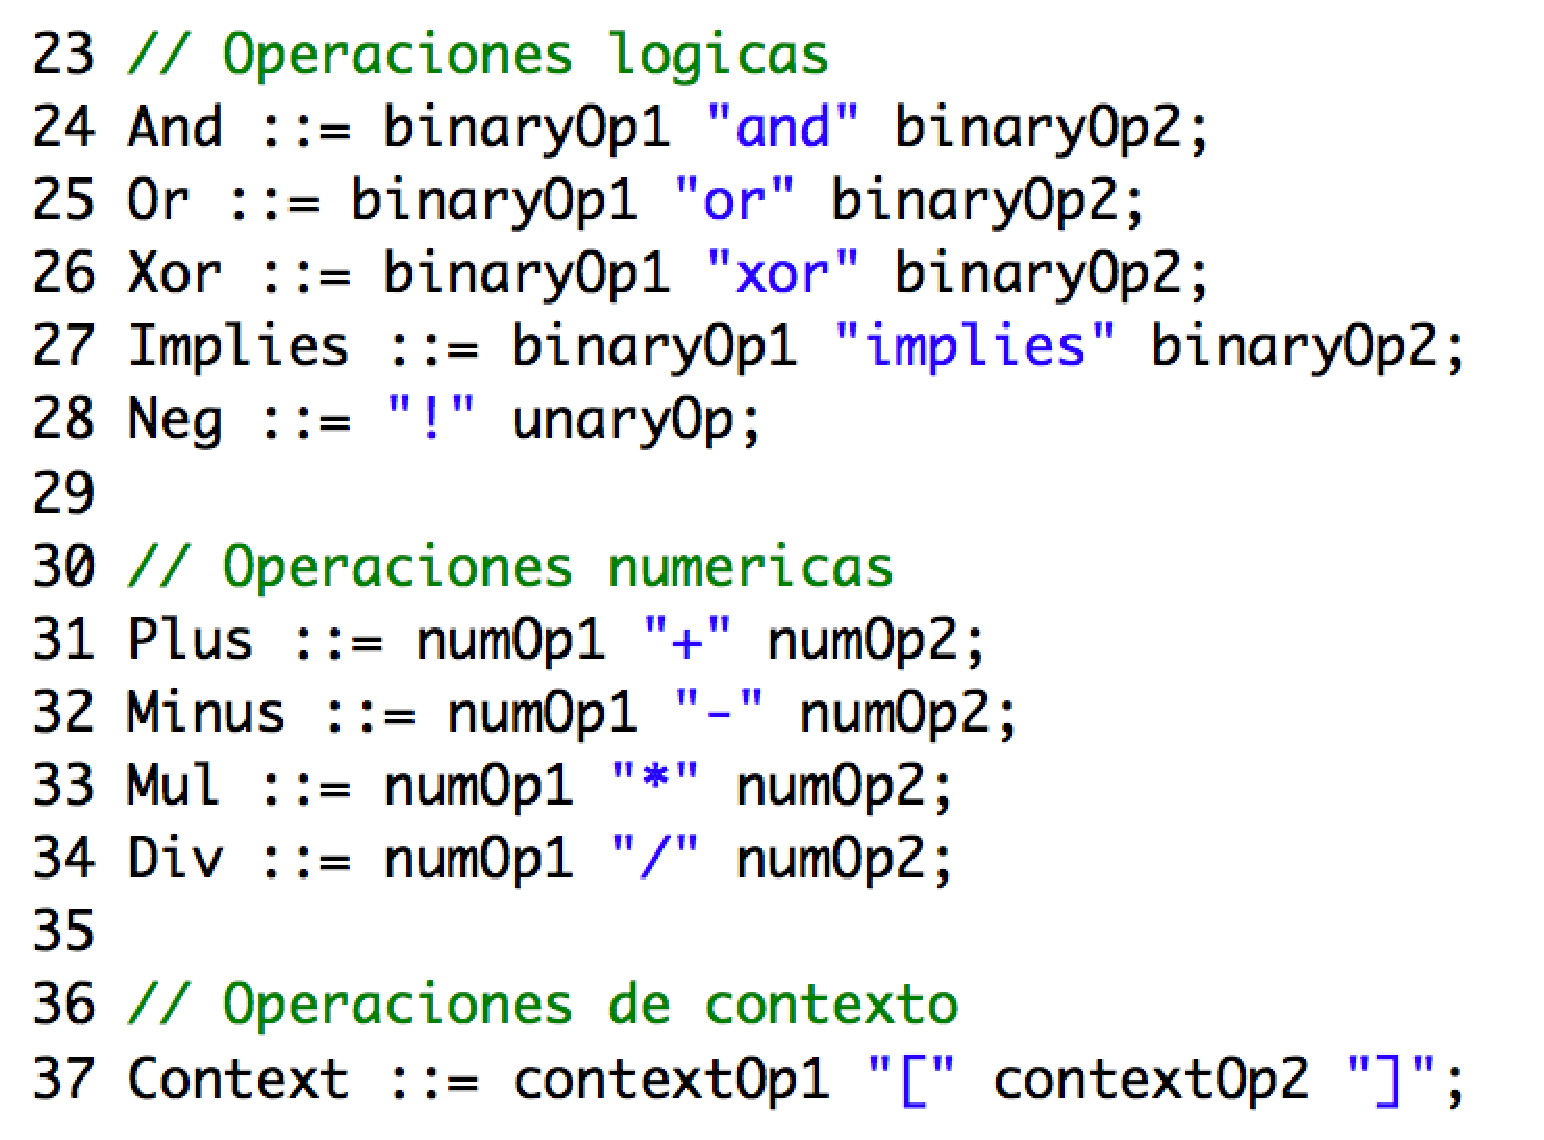
\includegraphics[scale=0.3]{gramatica/operaciones1.eps}
%    \caption{Implementaci�n de las operaciones de nuestro editor com EMFText}
%    \label{figopers}
%\end{figure}
%
%S� que cabe comentar con respecto a las operaciones las �ltimas l�neas, que muestran la asignaci�n de valor a las hojas de nuestros �rboles parseados. En esas l�neas estamos indicando que los atributos de las instancias de clase Number van a ser n�meros, y que los atributos de las instancias de las clases SimpleFeature y MultipleFeature van a ser palabras.
%
%La parte m�s complicada corresponde a la implementaci�n del inicio de la gram�tica y de las producciones que conducen a la misma. Pero antes de mostrar la figura con esta parte de la gram�tica conviene explicar el problema que llev� a realizar los cambios en el metamodelo mencionados en el cap�tulo anterior. Este problema surgi� a la hora de implementar las operaciones con prioridad, es decir, la inclusi�n de los par�ntesis.
%
%El inconveniente es que el tipo de gram�tica LL que implementa EMFText hac�a imposible tomar una decisi�n sobre hacia qu� elemento seguir parseando en caso de encontrarnos con un par�ntesis. La mejor soluci�n que se nos ocurri� para evitar este problema fue la adici�n de diversas clases y relaciones auxiliares en el metamodelo, cuya �nica funci�n es estructural y de apoyo a la gram�tica. Gracias a ellas y a una mejor definici�n de las producciones conseguimos evitar esos problemas de parsing y podemos llevar a cabo las operaciones de prioridad con par�ntesis.
%
%Las clases a�adidas para solventar esta situaci�n fueron las siguientes: BoolPriorityOperand1, BoolPriorityOperand2, NumPriorityOperand1, NumPriorityOperand2, BoolOperandChoices y NumOperandChoices. Las relaciones a�adidas fueron boolPriorityOp1, boolPriorityOp2, numPriorityOp1 y numPriorityOp2.
%
%Una situaci�n similar fue la que propici� que las operaciones Context, All y Any hayan sido dise�adas tal y como presenta el metamodelo, ya que que la particular sintaxis de estas (diferente a las dem�s que siguen el mismo esquema de op + char + op) tambi�n mostraba ciertos problemas de parsing. En este caso no fue necesario a�adir elementos auxiliares, sino simplemente recolocarlos para evitar estos problemas. Con esto ya se han hecho todos los cambios en el metamodelo, que alcanza en este punto su versi�n final tal como muestra la figura \ref{figmetameta}. Con respecto al metamodelo solamente quedan por comentar los m�todos que muestran algunas clases, que ser�n explicados en los pr�ximos cap�tulos ya que se usan en el proceso de validaci�n y sem�ntica.
%
%
%
%Una vez comentados estos detalles es momento de explicar el inicio de la gram�tica, que se muestra en la figura \ref{figinitgram}.
%
%En la primera l�nea y mediante la cla�sula SYNTAXDEF indicamos la extensi�n que queremos que tengan los ficheros escritos en nuestro lenguaje. En nuestro caso nos hemos decantado por la terminaci�n .hydraConst. En la segunda l�nea y mediante la cla�sula FOR se indica la URI del metamodelo. Una URI es un formato de direcci�n interno de Eclipse, que se usa para localizar otros ficheros en el workspace. En la tercera l�nea, delimitada por la cla�sula START, indicamos a la gram�tica que la clase inicial de nuestro metamodelo (y la que ser� la raiz en todos los �rboles parseados) es Model.
%
%El bloque OPTIONS permite activar algunas opciones de configuraci�n que incluye EMFText. En nuestro caso la �nica que tiene utilidad es usePredifinedTokens, que permite ahorrarnos la definici�n del token text. El bloque TOKENS sirve para definir los tokens de nuestra gram�tica. En nuestro caso usaremos 3: DIGIT para asignar al valor num�rico, TEXT para asignar a las caracter�sticas y DIRECCION para asignar la direcci�n f�sica del modelo de caracter�sticas.
%
%Por �ltimo, el bloque RULES permite crear las producciones. Como inicial, tal y como se especific� en los requisitos, exigimos un import y una direcci�n, que ser� almacenada en el atributo featureList de la clase Model. En la l�nea inicial tambi�n se indica, mediante una expresi�n regular, que el n�mero de restricciones a definir puede ser tan grande como se desee y que estas deben acabar con el car�cter '';'' .
%
%\begin{figure}[t]
%    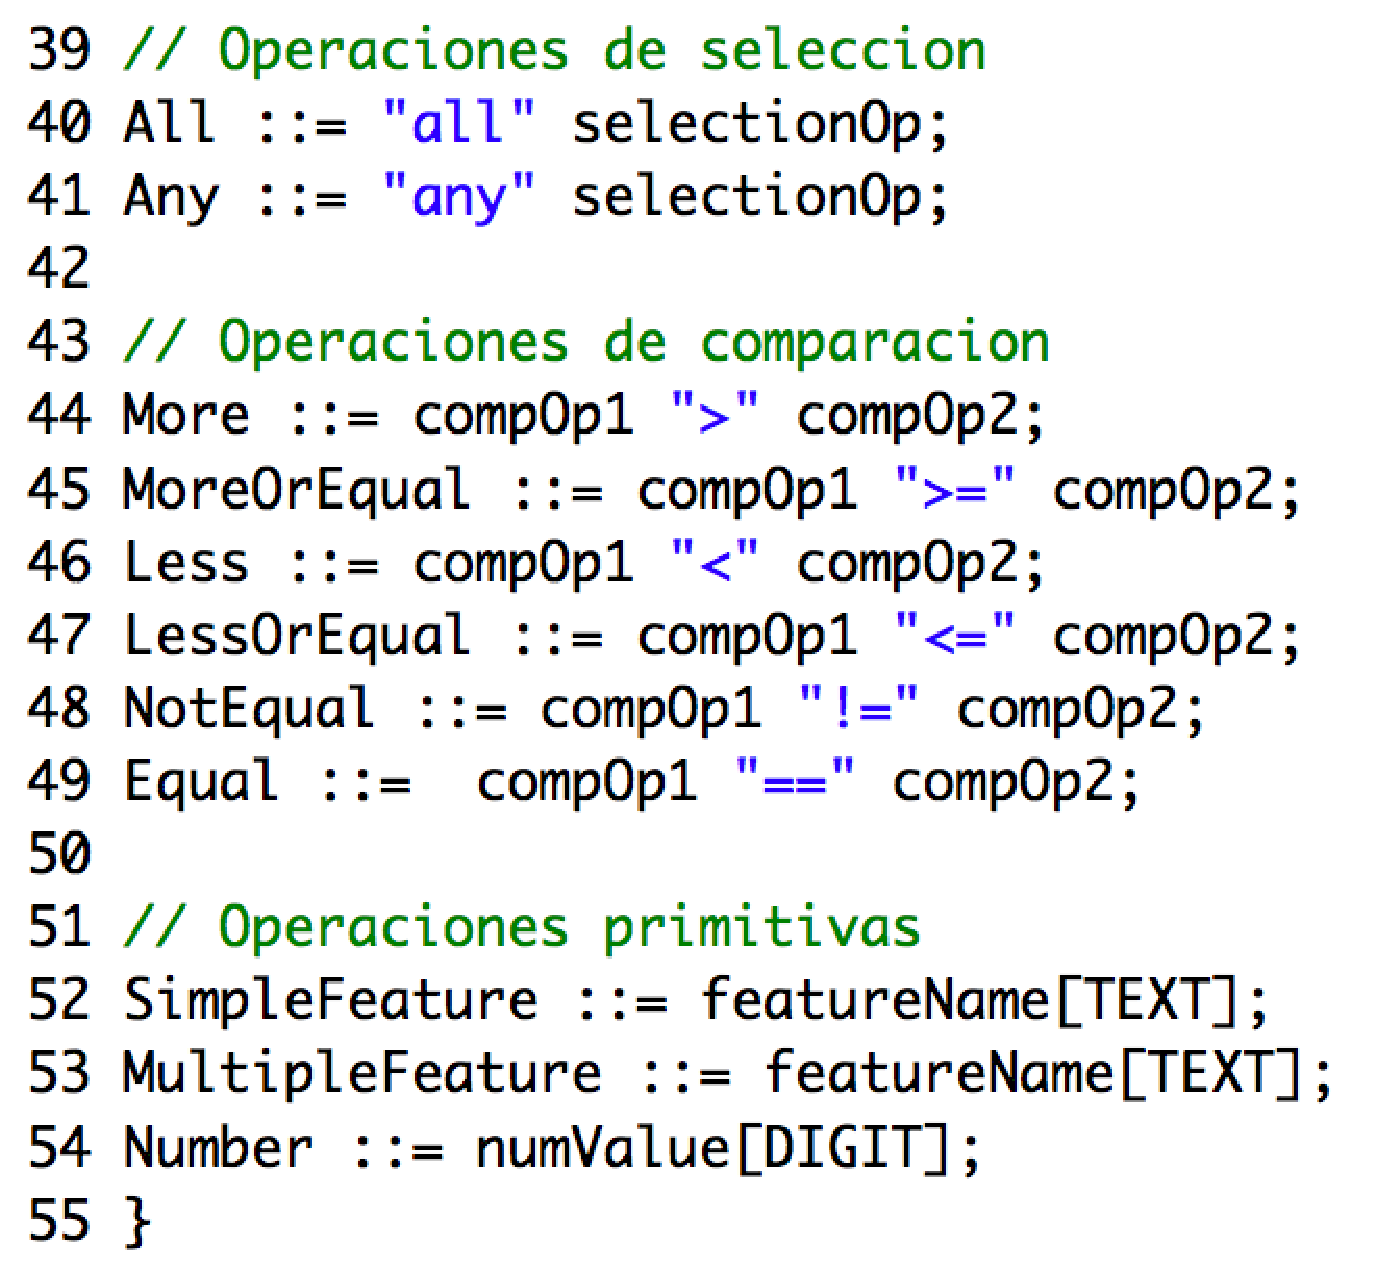
\includegraphics[scale=0.3]{gramatica/operaciones2.eps}
%    \caption{Implementaci�n de las operaciones de nuestro editor com EMFText}
%    \label{figopers}
%\end{figure}
%
%La l�nea de producci�n de Constraint diferencia entre operaciones con prioridad y sin ella. Sin el problema comentado de EMFText la gram�tica podr�a quedar as�, pero para solucionarlo nos vemos obligado a incluir las cuatro l�neas siguientes, cuya �nica funci�n es solventar esa situaci�n. El resto de la gram�tica continuar�a en la figura \ref{figopers} mostrada anteriormente, y ah� terminar�a.






\section{Pruebas}
\label{sec:gram:pruebas}
%%==================================================================%%
%% Author : Tejedo Gonz�lez, Daniel                                 %%
%%          S�nchez Barreiro, Pablo                                 %%
%% Version: 1.0, 25/11/2012                                         %%
%% Version: 1.0, 06/02/2013                                         %%
%%                                                                  %%
%% Memoria del Proyecto Fin de Carrera                              %%
%% Sintaxis abstracta,  pruebas                                     %%
%%==================================================================%%

Una vez creado nuestro metamodelo, deb�amos probar que dicho metamodelo era correcto. Es decir, que permit�a especificar todas las restricciones que dese�bamos crear, a la vez que, por construcci�n, imped�a la especificaci�n de restricciones que deb�an ser consideradas como sint�cticamente incorrectas.

Para ello realizamos una serie de pruebas consistentes en la creaci�n de varias instancias del metamodelo y observar el �rbol de sintaxis abstracta generado, comprobando si �ste se correspond�a con el esperado.

\begin{figure}[t]
    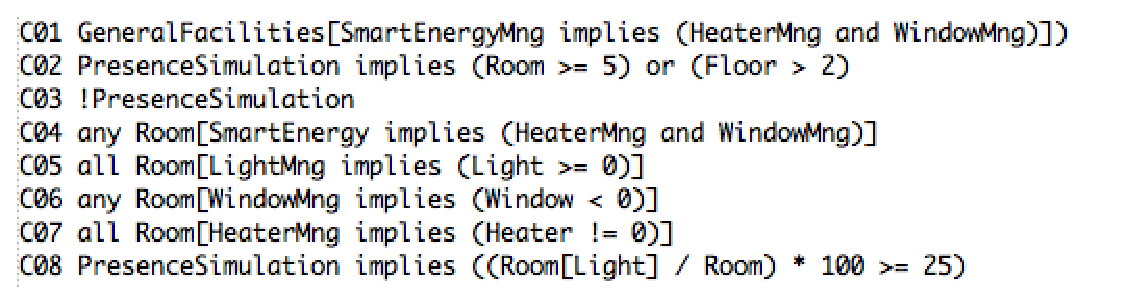
\includegraphics[scale=0.6]{metamodelo/instpruebas.eps}
    \caption{Conjunto de instrucciones que puso a prueba el funcionamiento del metamodelo}
    \label{figmetains}
\end{figure}

Las instrucciones que fueron puestas a prueba fueron las que se ven en la Figura~\ref{figmetains}. Este conjunto de instrucciones servir�n como pruebas tambi�n en momentos m�s avanzados del desarrollo. Dicho conjunto de pruebas fue dise�ado para recoger de la forma m�s exhaustiva posible todas las combinaciones de metaclases posibles.


% Cap�tulo 6: Discusi�n, Conclusiones y Trabajos Futuros
% \todo{Cap�tulo 7: Discusi�n, Conclusiones y Trabajos Futuros}

% CONTENT: Appendices, if desired
% \renewcommand\chaptername{Appendix}                      % hereafter, chapters are called "Appendix"
\renewcommand\thechapter{\Alph{chapter}}        % chapter number in Romans
\renewcommand\thesection{\Alph{chapter}.\alph{section}}  % make sections "I.a", instead of "1.1"
\setcounter{chapter}{0}                                  % start numbering chapters from 1 on again


% Appendix A:
% \input{populo/populo.tex} % Appendix I

% CONFIG: Bibliography style
% \cleardoublepage                            % start in right side page
\addcontentsline{toc}{chapter}{References}  % add this "chapter" to the ToC, with the name "Bibliography"
%\bibliographystyle{alpha}                  % bibliography style
\bibliographystyle{abbrv}                  % bibliography style
\bibliography{references/references}

\end{document}
